
%\documentclass[article]{jss}	% requires jss.bst, jss.cls, and jsslogo.jpg 
\documentclass[nojss]{jss}

%% -- LaTeX packages and custom commands ---------------------------------------

%% recommended packages
\usepackage{orcidlink,thumbpdf,lmodern}

%% further package
\usepackage{amsmath,amssymb,amsfonts,amsthm}	% Typical maths resource packages
\usepackage[T1]{fontenc}	% Output font enconding for letters of European languages
\usepackage[utf8]{inputenc}	% Use German umlaut input directly, codes documents in UTF-8
\usepackage{multirow}		% Create multirows in tables
\usepackage{rotating}		% Rotate text
\usepackage{enumitem}		% Control layout of itemize, enumerate, description
\usepackage[flushleft]{threeparttable} % No hanging indentation on table notes 

%% handle graphics
\usepackage{tikz}				% Create graphics programmatically
\usetikzlibrary{patterns}
\usetikzlibrary{positioning,shadings}
\usetikzlibrary{arrows}
\usetikzlibrary{shapes.multipart}

%% new custom commands
\newcommand{\class}[1]{`\code{#1}'}
\newcommand{\fct}[1]{\code{#1()}}


%% -- Article metainformation (author, title, ...) -----------------------------

%% - \author{} with primary affiliation (and optionally ORCID link)
%% - \Plainauthor{} without affiliations
%% - Separate authors by \And or \AND (in \author) or by comma (in \Plainauthor).
%% - \AND starts a new line, \And does not.
\author{Lennart Empting~\orcidlink{0009-0004-5068-4639}\\University of Duisburg-Essen}
\Plainauthor{Lennart Empting}

%% - \title{} in title case
%% - \Plaintitle{} without LaTeX markup (if any)
%% - \Shorttitle{} with LaTeX markup (if any), used as running title
\title{The \pkg{pvars} \proglang{R}-Package: VAR Modeling for Heterogeneous Panels}
\Plaintitle{The pvars R-Package: VAR Modeling for Heterogeneous Panels}
\Shorttitle{\pkg{pvars}: VAR Modeling for Heterogeneous Panels}

%% - \Abstract{} almost as usual
\Abstract{
	\pkg{pvars} offers a seamless implementation of vector autoregressive (VAR) methods for heterogeneous panel data. The \textsf{R}-package comprises \textit{panel cointegration rank tests} which can account for \textit{cross-sectional dependence} and for \textit{structural breaks} in the deterministic terms. The implemented \textit{panel SVAR models} can be estimated under these specifications with \textit{pooled cointegrating vectors} and identified by various \textit{panel identification procedures}. In this article, we review these methods and present their modular implementation in \textsf{R}. Two empirical illustrations reproduce examples from the literature step-by-step and guide the \pkg{pvars} user into conducting own analyses.
}

%% - \Keywords{} with LaTeX markup, at least one required
%% - \Plainkeywords{} without LaTeX markup (if necessary)
%% - Should be comma-separated and in sentence case.
\Keywords{panel cointegration rank tests, panel vector autoregressive models, pooled cointegrating vectors, structural identification, independent components, \proglang{R}, \pkg{pvars}}
\Plainkeywords{panel cointegration rank tests, panel vector autoregressive models, pooled cointegrating vectors, structural identification, independent components, R, pvars}

%% - \Address{} of at least one author
%% - May contain multiple affiliations for each author
%%   (in extra lines, separated by \emph{and}\\).
%% - May contain multiple authors for the same affiliation
%%   (in the same first line, separated by comma).
\Address{
  Lennart Empting\\
  Faculty of Economics\\
  Universität Duisburg-Essen\\
  Universitätsstraße 12\\
  45141 Essen, Germany\\
  E-mail: \email{lennart.empting@vwl.uni-due.de}\\
  URL: \url{https://www.github.com/Lenni89}
}

\begin{document}

%% -- Introduction -------------------------------------------------------------

%% - In principle "as usual".
%% - But should typically have some discussion of both _software_ and _methods_.
%% - Use \proglang{}, \pkg{}, and \code{} markup throughout the manuscript.
%% - If such markup is in (sub)section titles, a plain text version has to be
%%   added as well.
%% - All software mentioned should be properly \cite-d.
%% - All abbreviations should be introduced.
%% - Unless the expansions of abbreviations are proper names (like "Journal
%%   of Statistical Software" above) they should be in sentence case (like
%%   "generalized linear models" below).


\section{Introduction} \label{sec:Intro}
%%% INTRODUCTION OF TOPIC %%%
The ever-increasing availability of macroeconomic data and recent developments in the multivariate time series analysis for panels have popularized panel vector autoregressive methods in applied econometric research. The \pkg{pvars} package summarizes a toolkit for the empirical analysis on panels in the narrow sense, where the same time series variables are repetitively observed across several individual entities such as countries. This three-dimensional data structure thus contrasts with panels in a wider sense, where time series are just arranged along the same periods. Although \pkg{pvars}' application is not bounded to financial or macroeconometric research, it addresses the data properties typically found in macroeconomic panels, namely (i) \textit{mostly heterogeneous} (ii) \textit{endogenous interactions} between (iii) potentially \textit{non-stationary} variables. Since (iv) the \textit{time dimension is distinctively larger} than the cross-section, the time series are prone to (v) a \textit{complex deterministic term} with structural breaks in their mean and linear trend. The individual entities are usually subject to (vi) \textit{cross-sectional dependencies}.\footnote{See \citet{Pedroni2019} for an intuition and discussion of these panel properties and an overview on recent developments of single-equation and system-based methods. The data characteristics can be found in the applied econometrics of climate \citep{Pretis2020}, energy \citep{SmythNarayan2015}, and growth linked to financial development \citep{ChristopoulosTsionas2004} or public capital \citep{EmptingHerwartz2021b}.}

%%% APPROACHES FOR HETEROGENEOUS PANELS %%%
In order to deal with these data properties, the econometric literature extends individual time series methods by the cross-sectional dimension under selective pooling assumptions. For example, the panel methods implemented by the \proglang{Stata} commands \pkg{xtcointtest} \citep{StataCorp2019}, \pkg{xtwest} \citep{PersynWesterlund2008}, and \pkg{xtpmg} \citep{BlackburneFrank2007} originate from the single-equation framework comprising residual-based cointegration tests and autoregressive distributive lag (ARDL) models in error-correction representation. 
In contrast, \pkg{pvars} relies on vector autoregressive (VAR) models as a system of equations. This approach has the advantage of avoiding restrictive exogeneity assumptions on the variables and modeling their dynamics and interactions explicitly.
The model in vector error correction representation (VECM) can further accommodate multiple long-run relations and different types of deterministic regressors within the cointegration. Particularly the cointegration relations are reasonable candidates for a panel-wide pooling, while short-run dynamics are usually assumed to differ across individuals. 

%%% NICHE IN THE ECOSYSTEM OF R-PACKAGES %%%
The synthesis of VAR models and methods for heterogeneous panels has not been implemented yet, but many packages for \proglang{R} \citeyearpar{RCore2020} can already contribute specifications results and individual counter-checks. Hence, they may be subsumed into two pillars for \pkg{pvars}: Firstly, the \pkg{vars}-ecosystem with \pkg{urca} \citep{Pfaff2008}, \pkg{vars} \citep{Pfaff2008a}, and \pkg{svars} \citep{LangeEtAl_fc} covers individual VAR methods such as VECM and structural identification. The second pillar are the single-equation panel methods from \pkg{plm} \citep{CroissantMillo2008} such as dynamic panel regression models and panel unit root tests. Univariate panel time series can be tested for common or idiosyncratic non-stationarity using the more specialized package \pkg{PANICr} \citep{Bronder2016}. Like \pkg{pvars}, the \proglang{R}-package \pkg{panelvar} \citep{SigmundFerstl2019} and its \proglang{Stata}-equivalent \pkg{pvar} \citep{AbrigoLove2016} rest on the two pillars. However, they focus on stationary panels that contain more individuals than periods ($ N > T $), and the implemented estimators rely on slope coefficients that are homogeneous across all individuals in the PVAR model. Hence, they rather suit microeconomic applications, and their primary task is to deal with the \textit{\citeauthor{Nickell1981} bias} \citeyearpar{Nickell1981}.\footnote{See also \citet{CanovaCiccarelli2013} for a survey on panel VAR models.} 

%%% OBJECTIVE: CONTRIBUTION OF THIS PACKAGE %%%
The objective of \pkg{pvars} is to close the gap in the \pkg{vars}-ecosystem and provide a seamless implementation of the fruitful panel VAR methodology. For this, three fields of VAR applications are integrated into \pkg{pvars}, namely  panel estimation, cointegration testing, and structural identification. The implemented methods particularly noteworthy for each application field are (1) panel VECM with \textit{pooled cointegrating vectors} from Breitung's \citeyearpar{Breitung2005} two-step estimator. (2) The new panel cointegration rank tests by Arsova and Örsal \citeyearpar{ArsovaOersal2017,ArsovaOersal2018} respect cross-sectional dependencies stemming from common factors. \citet{ArsovaOersal2020} consider also structural breaks in the deterministic term. (3) Data-driven identification methods based on \textit{independent component analysis} (ICA) are extended for panels by \citet{CalhounEtAl2002} and \cite{Herwartz2017}.

%%% STRUCTURE OF THE ARTICLE %%%
The remainder of this article is structured as follows: Section~\ref{sec:Review} is a review on the econometric methods which are relevant for using this \proglang{R}-package. Section~\ref{sec:Implementation} highlights the available functions in \pkg{pvars}, their implementation, and their library of auxiliary functions. In Section~\ref{sec:Illustration}, we demonstrate two empirical applications of \pkg{pvars} to exemplary data from the reviewed articles. Section~\ref{sec:Summary} summarizes this article. \pkg{pvars} can be directly installed from the \textit{Comprehensive R Archive Network} \href{https://CRAN.R-project.org/package=pvars}{(CRAN)} and is shipped with a documentation for further help.



 
\section{Review of the econometric methodology} \label{sec:Review}
%%% OBJECTIVE %%%
A main motivation for combining multivariate time series from individual entities by panel methods is to increase the sample size and thereby extend the available information set for a more precise estimation and higher test power.
%%% POOLING APPROACHES %%%
Table~\ref{tab:pcoint} provides an overview of the literature of panel cointegration rank tests. In this unifying framework, the rows of the table classify the \textit{pooling approach} according the different stages of hypothesis testing, at which the the cross-section information is presumed to be homogeneous. The listed pooling approaches allow for increasing heterogeneity between the individuals: (1)~Panel-homogeneous cointegrating vectors enable a pooled estimation of these long-run coefficients. (2)~The averaged statistic is standardized by moments of the distribution which the individual statistics have in common.\footnote{In fact, the univariate counterpart by \citet[p.~59, Remark~3.1]{ImPesaranShin2003} allows for individual-specific test distributions if their third moments exist. The approximating gamma distribution with its well-defined moments suggests that this holds true for cointegration rank tests. By the Lyapunov central limit theorem, the cross-sectional average of their first and second moments can then be used instead. In light of this, future studies may extend JMN \citeyearpar{JohansenEtAl2000} and KN \citeyearpar{KuritaNielsen2019} to panel tests with individual deterministic terms.} Finally, (3)~the meta-analytical combination of individual $p$-values is the most flexible approach, where the commonality aims at a consistent test decision under an increasing number of individuals. If the alternative hypothesis is true, a non-vanishing share of individuals must actually exhibit this property.

\begin{table}[ht]	% tab:pcoint
	\centering
	\caption{Panel tests for the rank of cointegration.}
	\resizebox{\textwidth}{!}{ 
		
\begin{threeparttable}
	\begin{tabular}{ll|l|ll|ll}
		\hline\hline
		&  & \multicolumn{1}{|c|}{ \textbf{First generation} } & \multicolumn{2}{|c}{ \textbf{Second generation} } & \multicolumn{2}{|c}{ \textbf{Third generation} }  \\
		& \hfill \mbox{Cross-sectional dependence:} & Independence & Correlated errors & PANIC \citeyearpar{BaiNg2004} & Correlated probits & \\ 
		\multicolumn{2}{l|}{ \textbf{Pooling approach:} } &  &  &  &  & \\ 
		\hline
		\textbf{(1)} & Pooled coefficients & \citet{Breitung2005} & \tnote{a)}\quad $ LR(\Pi_C \mid \Pi_A) $ & --- & $ \times $ & \\[7pt]
		\textbf{(2)} & Averaged test statistics & Larsson et al.~\citeyearpar{LarssonEtAl2001} &  \tnote{a)}\quad $ LR(\Pi_B \mid \Pi_A) $  & Arsova, Örsal \citeyearpar{ArsovaOersal2018} & $ \times $  & \\
		&  & Örsal, Droge \citeyearpar{OersalDroge2014} &  & \tnote{b)}\quad PMSB\textsuperscript{Z} &  & \\[7pt]
		\textbf{(3)} & Meta-analytically & Maddala, Wu \citeyearpar{MaddalaWu1999} & \quad --- & Örsal, Arsova \citeyearpar{ArsovaOersal2017} & \citet{Hartung1999} &  \\
		&  combined $p$-values & \citet{Choi2001} &   & \tnote{b)}\quad PMSB\textsuperscript{F}, PMSB\textsuperscript{C}  & Arsova, Örsal \citeyearpar{ArsovaOersal2020} &  \\ 
		\hline\hline
	\end{tabular}
	\begin{tablenotes}
		\item \normalsize{\textbf{Not implemented in \pkg{pvars}:} The panel tests by a) Groen, Kleibergen \citeyearpar{GroenFrank2003} and b) Carrion-i Silvestre, Surdeanu \citeyearpar{SilvestreSurdeanu2011}.}
	\end{tablenotes}
\end{threeparttable}}
	\label{tab:pcoint}		
\end{table}

%%% GENERATIONS %%%
The columns of Table~\ref{tab:pcoint} represent the \textit{generations}, through which panel tests have evolved, and reflect the increasing complexity of the assumed data generating process. The first articles propose the plain approach for combining independent individual tests and thus are naive towards any dependencies between the individual entities. This cross-sectional dependence can emerge e.g.~between countries due to their trade and financial relations and is a research topic itself with regard to the global business cycle, the crude oil price, or other important commodities of the world market. The prevalent data property decreases the actual information content in macroeconomic panels compared to cross-independent samples of same size. First-generation tests then reject a correct null hypothesis more often than the nominal significance level and are thus ``over-sized''. In contrast, panel tests of the second generation maintain a correct test size and third-generation tests are robust against structural breaks additionally. For cointegration rank tests, the econometric literature considers structural breaks in the mean or linear trend of the cointegration relations. Empirical examples which are associated with shifts and with breaks in the linear time trend are the German reunification, the beginning of the Great Moderation, and its discussed end in the wake of the Great Recession. For a proper data representation, the VAR model must respect those changes in the long-run equilibrium, towards the error correction mechanism adjusts. Otherwise, the cointegration tests would miss to detect a reversion to the new equilibrium and thus understate the cointegration rank.

%%% BRANCHES / STRUCTURE OF THE REVIEW %%%
A third dimension of panel test construction is constituted by the underlying individual procedures, which have not been mapped onto Table~\ref{tab:pcoint}. These \textit{branches} are heterogeneous and often used side-by-side in a panel test article such that they do not follow such a clear pattern as the other two panel test properties do. This does not only hold for the example of cointegration tests, but also for VAR estimation and structural identification. All panel applications are confronted with similar construction problems and thus follow these dimensions in principle. Since the individual methods elude any classification scheme for Table~\ref{tab:pcoint}, Section~\ref{sec:Indiv} explains their technical details firstly and lays the foundation for Section~\ref{sec:Panel} presenting the panel methods along the two dimensions of Table~\ref{tab:pcoint}. The sections have the same structure according to estimation, testing, and identification as established in the individual and extended to the panel context respectively.

%%% NOTATIONS %%%
\textbf{Notations.} We adhere to the following rules. Subscript $ t = 1, \ldots, T $ denotes the periods and $ k = 1, \ldots, K $ refers to the endogenous variables in a multivariate time series. In order to simplify notation, Section~\ref{sec:Indiv} on the individual methods omits subscript $ i = 1, \ldots, N $ as the label specific to each of the $ N $ individuals. In contrast, Section~\ref{sec:Panel} uses subscript $ i $ to distinguish individual-specific elements also from homogeneous elements. Without any individual identifier $ i $, the latter must stay the same over the complete cross-section. Moreover, symbol $ \overset{d}{\longrightarrow} $ designates convergence in distribution. The $ (K \times (K-r)) $ matrix $ A_\perp $ is the orthogonal complement of a $ (K \times r) $ matrix $ A $ such that $ \text{rk} \lbrace [A : A_\perp] \rbrace = K $ indicates full rank and $ A_\perp'A=0 $. By convention, the orthogonal complement of a nonsigular square matrix is the zero matrix $ 0 $ and the orthogonal complement of zero matrix $ 0 $ is an identity matrix $ I_K $. With slight abuse of notation, integer $ r_\perp $ refers to the number of stochastic trends in a multivariate time series, corresponding to the cointegration rank $ r $.


\subsection{Individual methods} \label{sec:Indiv}
%%% VAR MODEL %%%
The basic unit for all presented panel methods is an individual VAR model of the form 
\begin{align} \label{eq:VAR}
	\boldsymbol{y}_{t} &= \Phi \boldsymbol{d}_{t} + A_1 \boldsymbol{y}_{t-1} + ... + A_p \boldsymbol{y}_{t-p} + \boldsymbol{u}_{t} \quad \textrm{with} \quad \boldsymbol{u}_{t} \sim (0,\Sigma_u) ,
\end{align}
where $\boldsymbol{y}_{t}$ is a vector of $ K $ stacked time series, $A_j, j=1,\ldots,p,$ are $ K \times K $ coefficient matrices for the VAR process of order $p$, and $ \Phi $ is a coefficient matrix for the deterministic regressors $ \boldsymbol{d}_{t} $. The errors $ \boldsymbol{u}_{t} $ are assumed to be serially, but not necessarily contemporaneously independent. Hence, the covariance matrix $ \Sigma_u $ is usually non-diagonal as the VAR model is estimated in reduced-form initially. Finding the structural shocks $ \boldsymbol{\epsilon}_{t} = \mathsf{B}^{-1} \boldsymbol{u}_{t} $, which exhibit no contemporaneous correlation, is the matter of structural identification in the the decomposition problem $ \Sigma_u = \mathsf{B} \mathsf{B}' $. The $ K $ variances of the structural shocks can be normalized to unity such that $ \boldsymbol{\epsilon}_{t} \sim ( 0, I_K ) $. Consequently, the unique identification of the impact matrix $ \mathsf{B}$ requires at least $ K(K-1)/2 $ restrictions on the $ K^2-K $ covariances in $ \Sigma_u $.

%%% VECM %%%
If $ \boldsymbol{y}_{t} $ is integrated of order $ I(1) $ at most and its first-differences $ \Delta \boldsymbol{y}_{t} $ are thus stationary, the VAR Model~\eqref{eq:VAR} in levels can be rewritten in its vector error correction representation
\begin{align} \label{eq:VECM}
\begin{split}
	\Delta \boldsymbol{y}_{t} \ & = \ \Phi \boldsymbol{d}_{t} + \Pi_{K} \boldsymbol{y}_{t-1} + \sum_{j=1}^{p-1} \Gamma_{j} \Delta \boldsymbol{y}_{t-j} + \boldsymbol{u}_{t} \quad \textrm{with} \quad \boldsymbol{u}_{t} \sim (0,\Sigma_u)
	\\ \textrm{using} & \quad \Pi_{K} := -I_K+\sum_{j=1}^{p} A_j \quad \textrm{and} \quad \Gamma_j := -\sum_{j^*=j+1}^{p} A_{j^*}, \ j=1,\ldots,p-1.
\end{split}
\end{align}
The $ K \times K $ coefficient matrix $ \Pi_{K} = \alpha\beta_{K}' $ of the error correction term summarizes the \mbox{$ K \times r $} cointegrating matrix $ \beta_{K} $ and loading matrix $ \alpha $, which adjusts the disequilibria in the $ r $ long-run cointegration relations $ \beta_{K}' \boldsymbol{y}_{t-1} $. The regressors $ \boldsymbol{d}_{t} $ of the deterministic term $ \Phi \boldsymbol{d}_t = \left[ \Phi_1 : \Phi_{2} \right] \left( \boldsymbol{d}_{1t}', \boldsymbol{d}_{2t}' \right)' $ are either unrestricted ($ \boldsymbol{d}_{2t} $) or restricted ($ \boldsymbol{d}_{1t} $) to the cointegration relations such that the coefficients $ \Phi_1 $ emerge from $ \Pi := \left[ \Pi_{K} : \Phi_1 \right] = \alpha \left[ \beta_{K}' : \beta_0' \right] = \alpha \beta' $. Finally, each $ \Gamma_{j} $ is a $ K \times K $ matrix of coefficients for short-run effects at lag $ j=1,\ldots,p-1 $.


\subsubsection{Estimating cointegrated VAR models} \label{sec:IndivEst}
\citet{Johansen1991,Johansen1996} provides a comprehensive collection of \textit{Maximum-Likelihood} methods for the individual VECM~\eqref{eq:VECM}. His ML-estimators and LR-tests are the foundation for any cointegrated VAR method of the \pkg{pvars} package. Hence, their definitions and components are throughout used in this article and shall be introduced here briefly. For convenience, firstly rewrite Model~\eqref{eq:VECM} in compact notation as
\begin{align} \label{eq:compactVECM}
\begin{split}
	Z_{0} \ & = \alpha\beta' Z_{1} + \Gamma Z_{2} + U \quad \text{now with} \quad \boldsymbol{u}_{t} \sim \mathcal{N}(0,\Sigma_u),
\end{split}
\end{align}
where the matrix $ \Gamma := \left[ \Gamma_1 : \cdots : \Gamma_{p-1} : \Phi_2 \right] $ lines up the coefficients for the short-run dynamics and for the unrestricted deterministic regressors. The observed time series are collected in the $ K \times T $ matrix $ Y := \left[ \boldsymbol{y}_{1}, \ldots, \boldsymbol{y}_{T} \right] $ for a sample $ 1,\ldots,T $ and the same holds for the error matrix $ U := \left[ \boldsymbol{u}_{1}, \ldots, \boldsymbol{u}_{T} \right] $, which contains no presample periods by construction of the estimation with lagging regressors. Accordingly, the regressand matrix is given by $Z_0 := \Delta Y $ and the two regressor matrices with $ T $ columns alike by
\begin{align} \label{eq:compactRegressor}
\begin{split}
	Z_1 := 
	\begin{bmatrix} 
		\boldsymbol{y}_{0}  & \ldots & \boldsymbol{y}_{T-1} \\ 
		\boldsymbol{d}_{11} & \ldots & \boldsymbol{d}_{1T} 
	\end{bmatrix}
	\quad \text{and} \quad
	Z_{2} \ & := 
	\begin{bmatrix}
		\Delta \boldsymbol{y}_{0}     & \ldots & \Delta \boldsymbol{y}_{T-1} \\
		                              & \vdots &                             \\
		\Delta \boldsymbol{y}_{1-p+1} & \ldots & \Delta \boldsymbol{y}_{T-p+1} \\
		\boldsymbol{d}_{21}           & \ldots & \boldsymbol{d}_{2T}
	\end{bmatrix}.
\end{split}
\end{align} 
The variables for the error correction term enter $ Z_1 $ in levels. $ Z_2 $ stacks the first-differenced and the unrestricted deterministic regressors. If $ p=1 $, all lagged $ \Delta \boldsymbol{y}_{t} $ drop out of $ Z_2 $. In conditional VECM, vectors of $ L $ (weakly) exogenous variables $ \boldsymbol{x}_t $ could be included as lagged $I(1)$ regressors into $ Z_1 $ as well as instantaneous and up to $ q $ lagged short-run effects into $ Z_2 $. The estimation would follow the same proceeding \citep[p.~398]{PesaranEtAl2000,Lutkepohl2005}, but we skip these terms here for the sake of notational brevity.


\textbf{ML-estimation.}\footnote{See \citet[Ch.~6]{Johansen1996}, \citet[Ch.~7.2.3]{Lutkepohl2005} and \citet[Ch.~3.1]{Lutkepohl2006} for a more detailed derivation and explanation.} The first order conditions from the maximized log-likelihood function
\begin{align} \label{eq:vecmLikeli}
\begin{split}
	\ln \mathcal{L} \left(\alpha, \beta, \Gamma, \Sigma_u \right) = & - \frac{KT}{2} \ln \left( 2\pi \right) - \frac{T}{2} \ln \left( \det ( \Sigma_u ) \right) \\
	& - \frac{1}{2} \text{tr} \left[ \left( Z_{0} - \alpha\beta' Z_{1} - \Gamma Z_{2} \right)' \ \Sigma_u^{-1} \ \left( Z_{0} - \alpha\beta' Z_{1} - \Gamma Z_{2} \right) \right]
\end{split}
\end{align} 
are solved for the estimators of VECM~\eqref{eq:compactVECM}, which corresponds to the following three steps:
\begin{enumerate}[label=\textbf{\arabic*.}]
	\item \textit{Concentrate out} short-run effects and the unrestricted deterministic term. The first step of $ \Pi $'s estimation is to remove the component $ \Gamma \boldsymbol{z_2}_t $ from $ \Delta \boldsymbol{y}_t $ and $ \boldsymbol{y}_t $ by OLS-regression of $ Z_0 $ resp. $ Z_1 $ on $ Z_{2} $. Using the Frisch-Waugh Theorem, the projection matrix $ M_2 := I_T - Z_2'(Z^{\ }_2 Z_2')^{-1} Z^{\ }_2 $ generates the ``long-run residuals'' $ R_{0} = Z_{0} M_2 $ resp. $ R_{1} = Z_{1} M_2 $ such that Model~\eqref{eq:compactVECM} collapses into the plain error correction model
	\begin{align} \label{eq:CoIntModel}
	\begin{split}
		Z_{0} M_2 & = \alpha\beta' Z_{1} M_2 + \Gamma Z_{2} M_2 + U M_2, \\
		R_{0} & = \alpha\beta' R_{1} + \widetilde{U}.
	\end{split}
	\end{align} 
	\item Estimate the concentrated Model~\eqref{eq:CoIntModel} by \textit{reduced-rank regression} (RRR) according to \citet{Anderson1951}.\footnote{See also \citet[Ch.~12.7]{Anderson2003} and \citet{Izenman1975}.} For doing so, define the moment matrices
	\begin{align} \label{eq:RRRmomat}
	\begin{split}
		S_{00} := \frac{R^{\ }_0 R_0'}{T}, \quad S_{01} := \frac{R^{\ }_0 R_1'}{T}, \quad \text{and} \quad S_{11} := \frac{R^{\ }_1 R_1'}{T}.
	\end{split}
	\end{align}
	Further inserting the OLS estimator~\eqref{eq:conOLS} for $ \widetilde{\alpha}(\beta) $ into the concentrated likelihood function transforms the ML maximization into the generalized eigenvalue problem
	\begin{align} \label{eq:RRReigen}
	\begin{split}
		\det \left( \lambda S_{11}^{\ } - S_{01}' S_{00}^{-1} S_{01}^{\ } \right) = 0.
	\end{split}
	\end{align} 
	This equation has $ K $ solutions with the ordered eigenvalues $ \lambda_1 \geq \lambda_2 \geq \ldots \geq \lambda_K \geq 0 $, which are the squared \textit{canonical correlation coefficients} and indicate the ``strength'' of cointegration in each solution. By the definition of cointegration, the correct coefficients $ \alpha\beta' $ must recombine the non-stationary $ R_{1} $ to the stationary $ R_{0} $. Hence, the estimator $ \widetilde{\beta} $ equals the eigenvectors of the $ r $ largest $ \lambda_j $ and is super consistent converging with rate $ T $ instead of the usual $ \sqrt{T} $ of the remaining OLS estimates. The $ r_\perp $ eigenvectors with the smallest $ \lambda_j $ are associated with the underlying stochastic trends and thus must cancel out from the henceforth \textit{rank-restricted} VECM.
	
	\item Maximize the log-likelihood function~\eqref{eq:vecmLikeli} conditional on a given $ \beta $, for which the super-consistent RRR-estimate $ \widetilde{\beta} $ can be inserted. The solution for the remaining estimators of the reduced-form VECM~\eqref{eq:compactVECM} are in fact \textit{conditional OLS}, namely
	\begin{align} \label{eq:conOLS}
	\begin{split}
		\widetilde{\Pi} & = \widetilde{\alpha} \beta' = \left[ R^{\ }_0 \left( \beta'R^{\ }_1 \right)' \left( \left( \beta'R^{\ }_1 \right) \left( \beta'R^{\ }_1 \right)' \right)^{-1} \right] \beta' = S_{01} \beta \left( \beta' S_{11} \beta \right)^{-1} \beta', \\
		\widetilde{\Gamma} & = \left( Z^{\ }_0 - \widetilde{\Pi} Z^{\ }_1 \right) Z_2'(Z^{\ }_2 Z_2')^{-1}, \\
		\widetilde{U} & = Z^{\ }_0 - \widetilde{\Pi} Z^{\ }_1 - \widetilde{\Gamma} Z^{\ }_2 = R^{\ }_0 - \widetilde{\Pi} R^{\ }_1.
	\end{split}
	\end{align}
\end{enumerate}
The residual covariance matrix is given by $ \widetilde{\Sigma}_u = \frac{\widetilde{U} \widetilde{U}'}{T} = S_{00} - \widetilde{\Pi} S'_{01} $ for ML estimation and is further corrected for $ n $, the number of coefficients per equation, in the OLS estimator $ \widehat{\Sigma}_u = \frac{T}{T-n} \cdot \widetilde{\Sigma}_u $. From Eq.~\eqref{eq:conOLS}, it becomes clear that only the loadings $ \widetilde{\alpha}(\beta) $ adjust towards the normalization of $ \beta $, while all other estimators are conditional on the complete matrix product $ \widetilde{\Pi} = \widetilde{\alpha} \beta' $. This shows that the cointegrated VAR process~\eqref{eq:VECM} and its impulse response functions (IRF) are invariant to any eligible normalization under a chosen rank $ r $ of $ \Pi $.


\textbf{GLS-based trend adjustment.} For the unique purpose of determining the cointegration rank, \citet{SaikkonenLutkepohl2000a} suggest to estimate and remove the deterministic term prior to an LM-test. \citet{SaikkonenLutkepohl2000c} apply the LR-statistic~\eqref{eq:LRrank} to the ``detrended'' time series, which may further improve the test power. This \textit{SL-procedure} entails a series of publications proposing different specifications of the deterministic term, which can be subsumed by the additive data generating process 
\begin{align} \label{eq:addDGP}
\begin{split}
	\boldsymbol{y}_{t} \ & = M_\mu \boldsymbol{d}_t + \boldsymbol{y}^{d \! t}_{t}, \\
	\boldsymbol{y}^{d \! t}_{t} \ & = A_{1} \boldsymbol{y}^{d \! t}_{t-1} + ... + A_{p} \boldsymbol{y}^{d \! t}_{t-p} + \boldsymbol{u}^{d \! t}_{t}.
\end{split}
\end{align}
Therein, the VAR process of the ``pure'' stochastic component $ \boldsymbol{y}^{d \! t}_{t} $ is usually abbreviated by a lag polynomial $ A(L) = I_K - A_1 L - \ldots - A_p L^p $. The $ K \times n_\mu $ matrix $ M_\mu $ collects the coefficients of the deterministic term in the moving-average representation of VAR~\eqref{eq:VAR}. Specifications of $ \boldsymbol{d}_t $ pursuant to the SL literature are listed in Table~\ref{tab:DetTerm} and illustrated in Section~\ref{sec:ERPT}.

%%% FGLS-ESTIMATION AS IN THE PVARS-PACKAGE %%%
All SL-procedures consider a \textit{GLS estimator} to determine $ M_\mu $. It becomes feasible by a preceding ML-estimation of VECM~\eqref{eq:VECM}, for which Table~\ref{tab:DetTerm} indicates also the conforming deterministic cases. Each hypothesis $ r_{H0} = 0,\ldots,K-1 $ in the test sequence then requires its specific rank-restriction on the ML-estimates and an own GLS estimation of $ M_\mu $. For this, the ML-estimates of the rank-restricted VECM are converted into $ \widetilde{A}_1, \ldots , \widetilde{A}_p $ of the VAR in levels and inserted into the transformed model
\begin{align} \label{eq:auxGLStrend}
\begin{split}
	{Q}' {A}(L) \boldsymbol{y}_t & = {Q}' {A}(L) M_\mu \boldsymbol{d}_t + {Q}' \boldsymbol{u}^{d \! t}_{t} \quad \text{for} \quad t=1,\ldots,T.
\end{split}
\end{align}
Therein, $ \boldsymbol{d}_t $ and $ \boldsymbol{y}_{t} $ are set to initial zeros in any presample period $ t \leq 0 $ and the feasible transformation matrix $ \widetilde{Q} $ is obtainable by inserting ML-estimates into
\begin{align} \label{eq:GLStrend}
\begin{split}
	Q & = \left[ \Sigma_u^{-1} \alpha \left( \alpha' \Sigma_u^{-1} \alpha \right)^{-1/2} : \alpha_\perp \left( \alpha_\perp' \Sigma_u \alpha_\perp \right)^{-1/2} \right].
\end{split}
\end{align}
The left-multiplication of $ {Q}' {A}(L) $ to \eqref{eq:addDGP} in \eqref{eq:auxGLStrend} allows for subtracting the confounding effects of the VAR dynamics and transforms the residual covariance matrix into $ I_K $. After vectorizing Model\eqref{eq:auxGLStrend}, $ M_\mu $ can thus be estimated by OLS. Alternatively, \citet[p. 438]{SaikkonenLutkepohl2000c} show that 
\begin{align} \label{eq:GLStrend2}
\begin{split}
	QQ' & \ = \ \Sigma_u^{-1} \alpha \left( \alpha' \Sigma_u^{-1} \alpha \right)^{-1} \alpha' \Sigma_u^{-1} + \alpha_\perp \left( \alpha_\perp' \Sigma_u \alpha_\perp \right)^{-1} \alpha_\perp' \ = \ \Sigma_u^{-1}.
\end{split}
\end{align} 
Accordingly, the GLS estimator based on the estimated covariance matrix $ \widetilde{\Sigma}_u $ can be applied directly to the data unaltered by $ \widetilde{Q} $, but still corrected for $ \widetilde{A}(L) $. Both proceedings lead to identical estimation results $ \widehat{M}_\mu $. Finally, the deterministic term is subtracted and the VECM of the stochastic component $ \boldsymbol{\hat{y}}^{d \! t}_{t} = \boldsymbol{y}_t - \widehat{M}_\mu \boldsymbol{d}_t $ is estimated by ML again -- now without any deterministic term. The usual LR-statistic~\eqref{eq:LRrank} can assess the sole null hypothesis of $ r_{H0} $, but its test distribution \eqref{eq:asympDistr} differs from the \citeauthor{Johansen1988} procedure.


\textbf{Deterministic term.} \citet{JohansenNielsen2018} distinguish between the \textit{innovative} and the \textit{additive} formulation of the deterministic term in Model~\eqref{eq:VECM} for the \citeauthor{Johansen1996} procedure resp.~in Model~\eqref{eq:addDGP} for the SL-procedure. Table~\ref{tab:DetTerm} adopts these labels and lists the model specifications. Like in a stable VAR process, the deterministic regressors $\boldsymbol{d}_t $ in VECM~\eqref{eq:VECM} can contain either no deterministic component, an intercept, or an additional linear trend. Beyond these ``standard'' types, non-stationarity and cointegration do complicate the estimation and testing in the presence of deterministic terms. For example, if a constant is assigned to $ \boldsymbol{d}_{2t} $, the unit roots in the VECM do not only accumulate the innovations $ \boldsymbol{u}_t $ into stochastic trends, but also this deterministic constant into a linear trend. On the other hand, the deterministic regressors $ \boldsymbol{d}_{1t} $ are restricted to the stationary cointegration relation and, thus, a linear trend in $ \boldsymbol{d}_{1t} $ does not generate a quadratic trend in the data. 
\begin{table}[ht]	% tab:DetTerm
	\centering
	\caption{Verified specifications of the deterministic term.}
	\resizebox{\textwidth}{!}{
		

\begin{threeparttable}
	\begin{tabular}{lll|l||ll}
		\hline\hline
		& \multicolumn{2}{c|}{ \textbf{Deterministic regressors} } & \multicolumn{2}{|c}{ \textbf{Type} } & \textbf{Literature} \\[4pt]
		& restricted $ \boldsymbol{d}_{1t} $ & unrestricted $ \boldsymbol{d}_{2t} $ & innovative\tnote{a)} \quad & additive\tnote{b)} &  \\ \hline
		\multicolumn{3}{l|}{$ \bullet $ \textit{\textbf{conventional:}}} & & & \\
		& none               & none                          & \textit{Case 1} & (needless) & --- \\
		& constant           & none                          & \textit{Case 2} & \textit{SL\_mean} & L\&S \citeyearpar[p.~185]{SaikkonenLutkepohl2000a} \\
		& none               & constant                      & \textit{Case 3} & \textcolor{gray}{\textit{SL\_ortho}} & \textcolor{gray}{S\&L \citeyearpar{SaikkonenLutkepohl2000} is irrelevant for \pkg{pvars}} \\
		& linear trend       & constant                      & \textit{Case 4} & \textit{SL\_trend} & L\&S \citeyearpar{SaikkonenLutkepohl2000a} \\
		& none               & constant \& linear trend      & \textit{Case 5} & --- & --- \\ \hline
		
		\multicolumn{3}{l|}{$ \bullet $ \textit{\textbf{period-specific:}}} & & & \\
		& none & seasonal dummies & + \textit{Case 2-5}      & + all & \citet[p.~84]{Johansen1996} ||  \ldots \\
		& impulse dummy & none & + all & + all & \quad \ldots TSL \citeyearpar[p.~348]{TrenklerEtAl2008} \\
		& shift dummy    & impulse dummies	& + \textit{Case 2} \tnote{c)} & + \textit{SL\_mean, SL\_trend} & JMN \citeyearpar[Ch.~3.2]{JohansenEtAl2000} || S\&L \citeyearpar{SaikkonenLutkepohl2000b}\tnote{d)} \\
		& trend break    & shift \& impulse dummies	   & + \textit{Case 4} & + \textit{SL\_trend} & JMN \citeyearpar[Ch.~3.1]{JohansenEtAl2000} || TSL \citeyearpar{TrenklerEtAl2008} \\ \hline\hline
	\end{tabular}
	\begin{tablenotes}
		\item[a)] Case labeling in accordance with \citet[Ch.~6.3]{Juselius2007} and \citet[p.~193]{HlouskovaWagner2010}.
		\item[b)] Overview on SL-test specifications from \citet[p. 24, Tab. 1; p. 25, Tab. 2]{Trenkler2008}.
		\item[c)] For shifts in \textit{Case 4}, \citet[JMN,][Ch.~4]{JohansenEtAl2000} assess $ r_{H0} $ under trend breaks and then restrictions on $ \beta_{0} $. 
		\item[d)] \citet[TSL,][]{LutkepohlEtAl2004} propose estimators of the unknown shift periods $ \boldsymbol{\tau} $.
	\end{tablenotes}
\end{threeparttable}


}
	\label{tab:DetTerm}		
\end{table}
In the additive formulation of the SL-procedure, the stochastic component contains the unit roots so that they do not interfere with the deterministic component. Irrespective of the accumulating innovations, the deterministic term thereby retains its intended specification, as it is visible in the data, and can be easily subtracted after FGLS estimation. For this, each row in Table~\ref{tab:DetTerm} juxtaposes the specifications of the additive model and the corresponding term in the innovative VECM~\eqref{eq:VECM} which provides the parameters in Eq.~\eqref{eq:auxGLStrend} to~\eqref{eq:GLStrend2} for feasible GLS estimation.

%%% PERIOD-SPECIFIC DETERMINISTIC REGRESSORS %%%
Additionally to the conventional types, there can be period-specific shifts in the mean and breaks in the linear trend as well as impulse dummies for a single period or a repeated pattern of dummies for deterministic seasonality. Both test procedures retain the conventional asymptotics in Eq.~\eqref{eq:asympDistr2} if solitary impulse dummies are added or if the seasonal dummies in $ \boldsymbol{d}_{2t} $ are centered around zero and thus accumulate along a constant. In contrast, only the distributions $ Z_{r_\perp} $ of the SL-procedure are invariant to the inclusion of shift dummies irrespective of their known or estimated shift period and both procedures must cope with the nuisance introduced by broken trend slopes. \citeauthor*{JohansenEtAl2000} (JMN, \citeyear{JohansenEtAl2000}), \citeauthor*{KuritaNielsen2019} (KN, \citeyear{KuritaNielsen2019}) as well as \citeauthor*{TrenklerEtAl2008} (TSL, \citeyear{TrenklerEtAl2008}) provide solutions for the Johansen- and SL-procedure respectively. Note that, beyond these specification whose asymptotics are verified by the literature of Table~\ref{tab:DetTerm} and described in Section~\ref{sec:IndivTest}, \pkg{pvars} accepts all period-specific extensions technically and does not check their validity for the cointegration tests.

Like for the conventional types in Table~\ref{tab:DetTerm}, any regressor $ \boldsymbol{d}_{1t} $ in the cointegration term has a first-differenced counterpart in $ \boldsymbol{d}_{2t} $. While the additive model separates clearly between deterministic and stochastic components, the innovative VECM~\eqref{eq:VECM} mixes the structural breaks into the autoregressive dynamics. Hence, the innovative model implies not only a single, but additional lagged first-differences of the break over the periods $ \tau, \tau+1, \ldots, \tau+(p-1) $ after the break occurring in period $ \tau $. Their coefficients depend on the other model parameters and would require non-linear estimation. Against this, all authors of the reviewed literature accept a minor loss in degrees of freedom and prefer to estimate these coefficients separately without those restrictions. Like TSL \citeyearpar[p.~335]{TrenklerEtAl2008}, \pkg{pvars} sets lagged impulse dummies for $ \tau, \ldots, \tau+p-1 $ in $ \boldsymbol{d}_{2t} $ even after a trend break because, in combination with the shift in $ \tau $, they control for these non-linear dynamics the same way as lagged shift dummies. In return, a subsequent FGLS estimation of $ M_\mu $ in the additive Model~\eqref{eq:addDGP} uses the regressor matrix $ \boldsymbol{d}_t $ without these lagged first-differences. Besides the conventional term, it contains only the trend break and shift at the very same period $ \tau $ as illustrated in Eq.~\eqref{eq:detTerm}.


\subsubsection{Testing the cointegration rank} \label{sec:IndivTest}
In order to determine the cointegration rank $ r $ in the $ K $-dimensional System \eqref{eq:VECM}, all testing procedures imply a sequential decision making according to the hypotheses 
\begin{align} \label{eq:RankHypo}
\begin{split}
	H_0: \text{rk}\left( \Pi \right) = r_{H0} & \text{\quad versus \quad} H_1: \text{rk} \left( \Pi \right) > r_{H0}, \quad r_{H0}=0, \ldots, K-1.
\end{split}
\end{align}
As long as a null hypothesis is rejected, $r_{H0}$ is increased by $1$ and tested again. The procedure stops for an accepted $ r = r_{H0} $ or if the maximal $r_{H0} = K - 1$ has been rejected in favor of $ r = K $. Correspondingly, the number of stochastic trends\footnote{Note that in the \proglang{R} code of \pkg{pvars} and also often in the considered literature the variable $d$ denotes the number of stochastic trends instead of the less ambiguous $ r_\perp $.} $ r_\perp = K - r_{H0} $ declines in each step from $K$ down to $1$. Note that, under a given $r_{H0}$, the \textit{maximum eigenvalue test} builds on the $ H_ 1 $ of $ \text{rk}(\Pi) = r_{H0} + 1 $ and the \textit{trace test} on $ \text{rk}(\Pi) = K $. Although both tests are applicable to panel extensions, only variants of the trace test have been adopted by the panel literature and are thus introduced here.


\textbf{LR-test.} \citet{Johansen1988} develops a nowadays predominant \textit{likelihood ratio} test which compares the maximized likelihood $ \mathcal{L}(r_{H0}) $ from the rank-restricted model against the likelihood $ \mathcal{L}(K) $ from the full-rank model with $ K $ variables. This trace statistic denotes as
\begin{align} \label{eq:LRrank}
\begin{split}
	\lambda^{\text{LR}} \left( r_{H0} \right) & = -2 \left[ \ln \mathcal{L}(r_{H0}) - \ln \mathcal{L}(K) \right] \\
	& = -T \sum_{j=r_{H0}+1}^{K} \ln(1-\hat{\lambda}_j) \ \overset{d}{\longrightarrow} \ Z_{r_\perp}. 
\end{split}
\end{align}
The estimated eigenvalues $ \boldsymbol{\hat{\lambda}} $ are the squared canonical correlation coefficients obtained from the RRR in Section~\ref{sec:IndivEst} and resemble the ordered eigenvalues of coefficient matrix $ \Pi $. Correspondingly, this test assesses whether any of the $ r_\perp $ smallest eigenvalues is significantly different from zero and thus increases the rank of $ \Pi $. Under $ H_0 $, the asymptotic test distribution is a function of $ r_\perp $-dimensional Brownian motions as outlined in Eq.~\eqref{eq:asympDistr}.


\textbf{LM-test.} Albeit its shadow existence in the individual time series methodology, the \textit{Lagrange multiplier} test adopted by \cite{LuukkonenEtAl1999} has proven useful for the panel test procedure proposed by \cite{Breitung2005} as it can serve as a vehicle to introduce the panel-homogeneous cointegrating vectors into an individual testing procedure. In order to make the cointegration rank $ r_{H0} $ testable by LM, the concentrated Model~\eqref{eq:CoIntModel} is extended by $ \phi \beta_\perp' R_{1} $ and multiplied by $ \alpha_\perp' $. Consequently in the auxiliary model
\begin{align} \label{eq:auxLMrank}
\begin{split}
	R_{0} & = \alpha \beta' R_{1} + \phi \beta_\perp' R_{1} + U^{{L \! M}} \\
	\text{resp. \quad}	\alpha_\perp' R_{0} & = \phi^* \beta_\perp' R_{1} + \alpha_\perp' U^{{L \! M}},
\end{split}
\end{align}
the extension is $ H_0: \alpha_\perp' \phi = \phi^* = 0_{r_\perp \times r_\perp} $ under $ r_{H0} $, but converts $ \Pi = \alpha \beta' + \phi \beta_\perp' $ into a full-rank matrix if the data suggest the alternative $ H_1: \text{rk}(\Pi) = K $. After inserting suitable estimates for the orthogonal complements,\footnote{For his panel cointegration test, \citet{Breitung2005} uses the individual first-step estimate for $ \alpha_i $ and the pooled second-step estimate for $ \beta_K $ under rank-restriction $ r_{H0} $. In \pkg{pvars}, their orthogonal complements are then calculated via the QR-decomposition as done in the \pkg{MASS} package \citep{VenablesRipley2002}.} the coefficient matrix $ \phi^* $ is estimated by OLS with regressand $ E := \widehat{\alpha_\perp}' R_0 $ and regressor $ W := \widehat{\beta_\perp}' R_1 $. The test statistic for $ H_0: \phi^* = 0 $ is constructed according to the here all-equivalent LR-, Wald-, or LM-principle and is thus directly calculated with
\begin{align} \label{eq:LMrank}
	\lambda^{\text{LM}} \left( r_{H0} \right) & = T \ \text{tr} \left[ EW' \left( WW' \right)^{-1} WE' \left( EE' \right)^{-1} \right] \ \overset{d}{\longrightarrow} \ Z_{r_\perp}.
\end{align}
This LM-test statistic and Johansen's LR-test statistic from Eq.~\eqref{eq:LRrank} are asymptotically identical and so are their test distributions.


\textbf{Test distribution.}\footnote{See \citet[Ch.~11.2]{Johansen1996}, \citet[Ch.~8.2]{Lutkepohl2005}, and \citet[p.~24, Eq.~2.9]{Trenkler2008}.} Under $ H_0 $ and $ T \to \infty $, the theoretical distributions converge to
\begin{align} \label{eq:asympDistr}
\begin{split}
	Z_{r_\perp} & = \text{tr} \left[ \int_0^1 \left(\text{d} W^\circ_{r_\perp} \right) W_{r_\perp}^{\bullet'} \ \left( \int_0^1 W^\bullet_{r_\perp} W_{r_\perp}^{\bullet'} \right)^{-1} \int_0^1 W^\bullet_{r_\perp} \left(\text{d} W^\circ_{r_\perp}\right)' \right]
\end{split}
\end{align}\\[-27pt]
\begin{align} \label{eq:asympDistr2}
\begin{split}
	\text{with \quad} W^\bullet_{r_\perp} & := 
	\begin{cases}
	W_{r_\perp} {\left( s \right)} & \text{for \textit{Case 1} or \textit{SL\_mean} } \\
	W_{r_\perp} {\left( s \right)} - \int_0^1 W_{r_\perp}{\left( s \right)}\text{d} s & \text{for \textit{Case 2} } \\
	\left[ \begin{smallmatrix}
	W_{r_\perp-1} {\left( s \right)} \\ s
	\end{smallmatrix} \right] - \int_0^1 \left[ \begin{smallmatrix}
	W_{r_\perp-1} {\left( s \right)} \\ s
	\end{smallmatrix} \right] \text{d} s & \text{for \textit{Case 3} } \\
	W_{r_\perp} {\left( s \right)} - sW_{r_\perp}{\left( 1 \right)} & \text{for \textit{Case 4} or \textit{SL\_trend}} \\
	\end{cases} \\
	\text{and \quad} \text{d} W^\circ_{r_\perp} & := 
	\begin{cases}
	\text{d} W_{r_\perp} {\left( s \right)} & \text{for \textit{SL\_mean} or any \textit{Case}} \\
	\text{d} W_{r_\perp} {\left( s \right)} - \text{d} sW_{r_\perp}{\left( 1 \right)} & \text{for \textit{SL\_trend}.} \\
\end{cases}
\end{split}
\end{align}
The $ r_\perp $-dimensional vector $ W_{r_\perp} {\left( s \right)} $ stacks the independent standard Brownian motions. In Eq.~\eqref{eq:asympDistr}, their vector products are integrated over their complete domain $ s \in [0,1] $. If the VECM accommodates deterministic regressors, $ W^\bullet_{r_\perp} {\left( s \right)} $ must be specified accordingly. Eq.~\eqref{eq:asympDistr2} lists the Brownian motions resp.~bridges for the conventional cases from Table~\ref{tab:DetTerm}. In contrast to those, trend breaks are specific to the periods of their occurrence and the relative position of these periods within the sample affects $ Z_{r_\perp} $ additionally. Also note that any unrestricted deterministic term which is accumulated under $ I(1) $, e.g.~the constant in \textit{Case 3}, dominates the stochastic trends and thus replaces a Brownian motion in $ W_{r_\perp} {\left( s \right)} $.

The asymptotic distribution of $ Z_{r_\perp} $ is non-standard, therefore critical values have been simulated e.g.~by \cite{OsterwaldLenum1992}. For this, $ W_{r_\perp} $ is substituted by a repetitive simulation of $ r_\perp $-dimensional vectors of Gaussian random walks with sufficiently\footnote{For example, \citet[Ch.~15]{Johansen1996} recommends $T=400$. \citet[p.~171, App.~B]{Breitung2005} employs $ T=500$ and \citet{OersalDroge2014} $ T=1000 $ in order to simulate the respective moments of $ Z_{r_\perp} $.} large sample size. Also, $ Z_{r_\perp} $ can be approximated by the gamma distribution $ \Gamma (\mathsf{s}, \mathsf{r}) $, whose continuous probability density function offers the advantage of retrieving $p$-values conveniently. In order to do so, its shape- and rate-parameters are equated with
\begin{align} \label{eq:GammaParameter}
\begin{split}
	\mathsf{s} = \frac{\mathbb{E}(Z_{r_\perp})^2}{ \text{Var}(Z_{r_\perp}) } \qquad \text{and} \qquad \mathsf{r} = \frac{\mathbb{E}(Z_{r_\perp})}{ \text{Var}(Z_{r_\perp}) }.
\end{split}
\end{align}
Simulated values for the moments $ \mathbb{E}(Z_{r_\perp}) $ and $ \text{Var}(Z_{r_\perp}) $ can be found for example in \citet{LarssonEtAl2001} and \citet{Breitung2005}.\footnote{\citet{LarssonEtAl2001} provide moments of $ Z_{r_\perp} $ only for \textit{Case~1} and \citet{Breitung2005} for \textit{Case~2} to \textit{Case~4} in order to center and scale the LR-bar panel test statistic as in Eq.~\eqref{eq:LRbar}. In \pkg{pvars}, these moments are stored in the list object \code{coint\_moments}.} Like the unknown theoretical distribution $ Z_{r_\perp} $, their simulation depends on \textit{(i)} the number of stochastic trends $ r_\perp $ under $ H_0 $, \textit{(ii)} the deterministic term, and \textit{(iii)} the number of weakly exogenous variables in a conditional VECM. Hence, the different test specifications imply a grid of simulation setups to run.

More flexibility towards adapting these specifications is offered by response surface approximation of the moments as employed by \citet{Doornik1998}. For each \textit{Case}, he estimates response surface coefficients\footnote{In \pkg{pvars}, the response surface coefficients are stored in the list object \code{coint\_rscoef}.} of a polynomial regression model $ f(r_\perp) $ which ``predicts'' the moments of $ Z_{r_\perp} $ for \citet{Johansen1996}. \citet{Trenkler2008} derives response surface coefficients specifically for the trend-adjusted tests of Eq.~\eqref{eq:addDGP}. TSL \citeyearpar{TrenklerEtAl2008} tabulate these coefficients for trend-adjusted tests which accommodate structural trend breaks in the conintegration relationship. Likewise, JMN \citeyearpar{JohansenEtAl2000} consider structural breaks in the constant and in the linear trend of the innovative model, which KN \citeyearpar{KuritaNielsen2019} generalize for conditional VECM by \citet[Ch.~9]{Doornik1998}. Although both models, additive and innovative, can cope with several breaks in principle, the regression models $ f \left(r_\perp, \frac{\boldsymbol{\tau}}{T} \right) $ by JMN \citeyearpar{JohansenEtAl2000}, KN \citeyearpar{KuritaNielsen2019}, and TSL \citeyearpar{TrenklerEtAl2008} contain polynomials of up to two break periods $ \boldsymbol{\tau} $ only. \pkg{pvars} resorts to the respective approximation automatically in order to comply with the test specification selected by the user.



\subsubsection{Identifying structure}
Based on the given rank-restriction $ r $ and structural shocks $ \boldsymbol{\epsilon}_{t} = \mathsf{B}^{-1} \boldsymbol{u}_{t} $, the VECM~\eqref{eq:VECM} can be transformed according to the \textit{Granger representation theorem} (GRT) into
\begin{align} \label{eq:GRT}
\begin{split}
	\boldsymbol{y}_{t} \ & = \ \Xi \mathsf{B} \sum_{j=1}^{t} \boldsymbol{\epsilon}_{j} + \sum_{j=0}^{\infty} \Xi^{*}_{j} \mathsf{B} \boldsymbol{\epsilon}_{t-j} + \Xi \Phi \sum_{j=1}^{t} \boldsymbol{d}_{j} + \sum_{j=0}^{\infty} \Xi^{*}_{j} \Phi \boldsymbol{d}_{t-j} + \boldsymbol{y}^{*}_{0} \quad \text{with} \\
	\Xi \ & = \ \beta_{\perp} \left[ \alpha_{\perp}' \left(I_K - \sum_{j=1}^{p-1} \Gamma_{j} \right) \beta_{\perp} \right]^{-1} \alpha_{\perp}'.
\end{split}
\end{align}
The initial vector $ \boldsymbol{y}^{*}_{0} $ and the deterministic terms are usually dropped in order to trace the responses to an isolated structural impulse $ \epsilon_{(k)} $. The number of stochastic trends $\text{rk}(\Xi) = K-r = r_\perp $ follows from the $ K \times r_\perp $ orthogonal complements $ \alpha_{\perp} $ and $ \beta_{\perp} $ for the $ K \times r $ loadings $ \alpha $ and cointegrating vectors $ \beta_K $. Their different specifications illustrate the role of the components in \eqref{eq:GRT} and their options for structural restrictions:
\begin{itemize}
	\item If $ r_\perp = 0 $, the stochastic trends cancle out and the sole multiplier matrices $ \Xi_j^* \mathsf{B} $ reflect the IRF of the implied \textit{stable} SVAR model. Hence, just-identification requires the $ K(K-1)/2 $ restrictions to be imposed on the instantaneous effects $\mathsf{B} $ exclusively. A simple example is \cite{Sims1980}, who assumes recursive (short-run) causality such that the structural effects on impact can be calculated by $ \widehat{\textsf{B}} = \text{chol} \left( \widehat{\Sigma}_{u} \right) $.
	
	\item If $ r_\perp = K $, VECM~\eqref{eq:VECM} loses its error correction term and is estimated as a first-differenced VAR model by OLS~\eqref{eq:conOLS}. Since $ \alpha_\perp = \beta_\perp = I_K $, matrix $ \Xi = \left(I_K - \sum_{j=1}^{p-1} \Gamma_{j} \right)^{-1} = \Gamma(1)^{-1} $ is full-rank and $ K(K-1)/2 $ long-run restrictions are sufficient for identifying this SVAR of \textit{growth rates} $ \Delta \boldsymbol{y}_{t} $. In this example, recursive long-run causality is imposed on the structural long-run effects $ \Xi \mathsf{B} $ such that $ \widehat{\textsf{B}} = \widetilde{\Gamma}(1) \ \text{chol}\left( \widehat{\Sigma}_{\infty} \right) $ is calculated via the long-run covariance $ \Sigma_\infty := \Xi \mathsf{B} \mathsf{B}'\Xi' = \Gamma(1)^{-1} \Sigma_u \Gamma(1)'^{-1} $. 
	
	\item A cointegration rank $ r $ implies $ r_\perp $ permanent shocks at minimum and conversely $ r $ transitory shocks at maximum. Identifications schemes in the tradition of \citet{KingEtAl1991} assume that $ \Xi \mathsf{B} $ is rank-deficient due to $ r $ columns of $ {\bf 0}_K $. Each $ {\bf 0}_K $ suppresses the stochastic trends and thus defines a transitory shock in $ \boldsymbol{\epsilon}_{t} $. Other formulations of the rank-deficiency may lead to fewer transitory shocks.
\end{itemize} 


\textbf{ML-estimation.}\footnote{See \citet{Vlaar2004}, who imposes linear short- and long-run restriction with restriction matrices for the cases of just- and over-identification. Compare also to \citet[Ch.~11, p.~331]{Hamilton1994}, \citet[Ch.~3.2, p.~84]{Lutkepohl2006}, and \citet[Ch.~11.2.2 and p.~315]{KilianLutkepohl2017} as a full-information MLE.} The impact matrix $ \mathsf{B} $ can be estimated by ML via $ \mathcal{L} \left(\alpha, \beta, \Gamma, \mathsf{B} \right) $ as an extension of Eq.~\eqref{eq:vecmLikeli}. Inserting the reduced-form estimates from Section~\ref{sec:IndivEst} facilitates a conditional ML-estimation of $ \mathsf{B} $ as Step~\textbf{4.} with the concentrated likelihood function
\begin{align} \label{eq:svecmLikeli}
\begin{split}
	\ln \mathcal{L}_c \left( \mathsf{B} \right) = & - \frac{KT}{2} \ln \left( 2\pi \right) - \frac{T}{2} \ln \left( \det ( \mathsf{B} ) \right)^2 - \frac{1}{2} \text{tr} \left[ \mathsf{B'}^{-1} \mathsf{B}^{-1} \widetilde{\Sigma}_u \right].
\end{split}
\end{align}
This constrained maximization problem has no closed-form solution. Hence, \cite{BreitungEtAl2004} maximize $ \mathcal{L}_c \left( \mathsf{B} \right) $ with respect to the free parameters subject to the identifying restrictions numerically by the scoring algorithm of \citet{AmisanoGiannini1997}. If the number of short- and long-run restrictions suffice just-identification only, the equality $ \widetilde{\Sigma}_u = \mathsf{\widetilde{B}} \mathsf{\widetilde{B}}' $ holds and the scoring algorithm serves as a non-linear equation solver.


\subsection{Panel methods} \label{sec:Panel}

\subsubsection{Estimating cointegrated VAR models}
In macroeconomic panels, the idiosyncrasies of countries can subvert the objective to increase estimates' precision with pooled data. Deterministic effects like intercepts are usually kept individual-specific in panel data analysis, but even the assumption of homogeneous slope coefficients can be too restrictive. \citet{PesaranSmith1995} demonstrates how systematic differences between individual dynamics lead to inconsistent estimates and consequently deny poolability. As an economically plausible middle ground, \citet{PesaranEtAl1999} propose a selective pooling for single-equation models, where only the long-run relationship is homogeneous across all individuals, while the short-run dynamics are considered as heterogeneous. The following panel estimators adopt this principle into a system of equations and restrict the $ r $ cointegrating vectors $ \beta_i = \beta \ \forall \ i $. Although the individual VECM~\eqref{eq:VECM} does not require the basic normalization of the error correction term as single-equation models do, a panel-wide normalization becomes necessary in order to extract the homogeneous $ \beta $ from the individual coefficient matrices $ \Pi_i = \alpha_i \beta' $.


\textbf{Two-step estimator.}\footnote{See also \citet[Ch.~7.2.2]{Lutkepohl2005} or \citet{BruggemannLutkepohl2005} about GLS estimation of the individual cointegration parameters. In fact, Eq.~\eqref{eq:2S_GLS} reduces to this GLS estimator if there is only $ N=1 $ individual entity. Moreover, \citet[Ch.~7.3.2]{Lutkepohl2005} and \citet[p.~159]{Breitung2005} consider restricted $ \beta $.} 
\citet{Breitung2005} extends the individual two-step estimator by \citet{AhnReisel1990} to a panel estimator for $\beta$. Based on the panel-wide normalization $\Pi_i = \alpha_i \left[I_r : \mathbf{B} \right] = \left[ \alpha_i I_r : \alpha_i \mathbf{B} \right] \ \forall \ i $, he transforms the concentrated Model~\eqref{eq:CoIntModel} into
\begin{align} \label{eq:2S_stack}
\begin{split}
	R^{\ }_{0,i} - \alpha_i I_r R_{1,i}^{(1)} & = \alpha_i \mathbf{B} R_{1,i}^{(2)} + U_{i} \text{\quad with \quad}
	R_{1,i} = \begin{bmatrix} R_{1,i}^{(1)} \\ R_{1,i}^{(2)} \end{bmatrix} \\
\end{split}
\end{align}
partitioned into $ R_{1,i}^{(1)} $ as the $ r $ upper time series and $ R_{1,i}^{(2)} $ as the remaining $ r_\perp $ time series and $ n_1 $ restricted deterministic regressors. The left-multiplication $ \alpha_{i}^{(+)} \alpha_i = I_r $ eliminates the individual loadings $ \alpha_{i} $ in Eq.~\eqref{eq:2S_stack} such that Model~\eqref{eq:CoIntModel} is further transformed into
\begin{align} \label{eq:2S_aux}
\begin{split}
	\alpha_{i}^{(+)} \left(R^{\ }_{0,i} - \alpha_{i} R_{1,i}^{(1)} \right) & = \mathbf{B} R_{1,i}^{(2)} + \alpha_{i}^{(+)} U_{i} \text{\quad using \quad} \alpha_{i}^{(+)} = \left( \alpha_i' \Sigma_{u,i}^{-1} \alpha_i \right)^{-1} \alpha_i' \Sigma_{u,i}^{-1}. \\
\end{split}
\end{align}
The \textit{pooled OLS estimator} of the homogeneous $ \mathbf{B} $, i.e.~the right $ r \times \left( r_\perp + n_1 \right) $ block of the normalized and transposed cointegrating matrix, yields the second step given by
\begin{align} \label{eq:2S_GLS}
\begin{split}
	\widehat{\mathbf{B}}_{2S} & = R_0^{(+)} R_1^{(2)'} \left( R_1^{(2)} R_1^{(2)'} \right)^{-1}
\end{split}
\end{align}
\begin{align}
	\text{with regressand} \quad R^{(+)}_{0,i} & := \alpha_{i}^{(+)} R^{\ }_{0,i} - R_{1,i}^{(1)} & \text{collected in} \quad R_0^{(+)} := \begin{bmatrix} R^{(+)}_{0,1} : \cdots : R^{(+)}_{0,N} \end{bmatrix} & \nonumber \\
	\text{and regressor} \quad R_{1,i}^{(2)} &  & \text{collected in} \quad R_1^{(2)} := \begin{bmatrix} R_{1,1}^{(2)} : \cdots : R_{1,N}^{(2)} \end{bmatrix} &. \nonumber
\end{align}
For feasible estimation, inserting any $ \sqrt{T} $-consistent estimates for $ \alpha_i $ and $ \Sigma_{u,i} $ leaves the limiting distribution of the estimator~\eqref{eq:2S_GLS} unaffected. This first step may be the individual ML-estimation of each VECM, which concentrates out the short-run effects and unrestricted deterministic terms $ \Gamma_i Z_{2,i} $ from the observed time series as well. Under rank-restriction $ r $, the second-step estimates $ \widehat{\mathbf{B}}_{2S}$ thereby $ T\sqrt{N} $-consistently \citep[p.~156, Th.~1]{Breitung2005}. Overall, this procedure thus follows the steps of the ML-estimation, but sets a pooled estimation on top of the individual reduced-rank regressions~\eqref{eq:RRReigen}. Like in third step of the individual ML-estimation, the cointegrating matrix $ \widehat{\beta}' = \begin{bmatrix} I_r : \widehat{\mathbf{B}}_{2S} \end{bmatrix} $ can be reintroduced into the conditional OLS~\eqref{eq:conOLS} of the individual parameters, for which product moments are already available from the first step. Thereof, the estimates for $ \alpha_i $ and $ \Sigma_{u,i} $ -- now conditional on the pooled $ \widehat{\beta} $ -- can be used in Eq.~\eqref{eq:2S_GLS} again. \citet[p.~195]{HlouskovaWagner2010} expand this principle and iterate conditional OLS and second-step estimation alternately until reaching convergence of the estimates $ \widehat{\mathbf{B}}_{2S} $.


\textbf{Deterministic term.} Since the first estimation step \eqref{eq:CoIntModel} removes the unrestricted regressors $ \boldsymbol{d}_{2,it} $ from the error correction Model~\eqref{eq:VECM}, the coefficients $ \Phi_{2i} $ are individual-specific by construction. In consequence, the homogeneity restriction $ \beta_{K,i} = \beta_K $ in 
\begin{align} \label{eq:2S_det}
\begin{split}
	\Pi_i := \left[ \Pi_{K,i} : \Phi_{1,i} \right] = \alpha_i \left[ \beta_{K}' : \beta_{0i}' \right] = \alpha_i \left[I_r^{\ } : \mathbf{B}_{\ }^{(2)} : \mathbf{B}_i^{(3)} \right]
\end{split}
\end{align}
implies one additional choice for specifying the innovative deterministic term in Table~\ref{tab:DetTerm}:\footnote{\citet[Ch.~4.1]{GroenFrank2003} give an overview on the different combinations that emerge from this single additional option.} 
The coefficients for $ D_{1,i} M_{2i} $ can be defined as having some homogeneous $ \beta_{0i} = \beta_{0} \ \forall \ i $ or individual-specific effects $ \beta_{0i} $. For example, \textit{Case 2} with heterogeneous intercepts $ \beta_{0i} $ and $ p_i = 1 \forall i $, i.e.~without the need to correct for lagged short-run effects by $ M_{2i} $, adds \textit{fixed-effects} to the auxiliary Model~\eqref{eq:2S_aux}. The regressors of such individual-specific $ \mathbf{B}_i^{(3)} $ are partialled out from the pooled regression beforehand, while $ \mathbf{B}^{(2)} $ is simply extended by the $ r \times n_1 $ homogeneous $ \beta_{0}' $ and estimated by the pooled $ \widehat{\mathbf{B}}_{2S} $ of \eqref{eq:2S_GLS}. Note however that $ \Phi_{1i} = \alpha_{i} \beta_{0}' $ remains heterogeneous irrespective of the homogeneity restriction on $ \beta_{0} $.


\subsubsection{Testing the cointegration rank}
Like the individual tests in Section~\ref{sec:IndivTest}, the following panel tests evaluate the hypothetical cointegration rank $ r_{H0}=0,...,K-1 $ within a sequential testing procedure. Each of the $ N $ individuals must have observations on the same $ K $ variables so that the hypothesis pair on the heterogeneous ranks $ r_i $ in the individual VAR processes $ \boldsymbol{y}_{it} $ can be stated as
\begin{align} \label{eq:Hypothesis}
\begin{split}
	H_0: \bar{r} = r_{H0} & \text{\quad versus \quad} H_1: \text{rk}\left( \Pi_i \right) > r_{H0} \ \text{for some} \ i \\
	\text{with} \ \bar{r} = & \max \{ \text{rk}\left( \Pi_i \right) \mid i=1,..,N \}.
\end{split}
\end{align}
While a statistical heterogeneity in $ r_i $ lets the sequential procedure find the maximum rank among the individual processes, the theoretical context might allow for the more restrictive assumption of homogeneous cointegration ranks across all individuals $ i=1,\ldots,N$. Accordingly, the hypothesis pair~\eqref{eq:Hypothesis} would adopt a common rank $ r_i = \bar{r} = r $. \citet[p.~9]{SilvestreSurdeanu2011} assume this ``for the panel data based procedure to make sense'' and the homogeneous cointegrating vectors $ \beta_{K,i} = \beta_K $ in \citet{Breitung2005} and \citet{GroenFrank2003} actually have the statistical implication of $ r_i = r $.


\textbf{Pooled cointegrating vectors.} The more restrictive assumption of homogeneous $ \beta_K $ allows for a pooled estimation to further increase the test power. Only in this case, the \textit{pooling} and the \textit{combination} approach of the panel test differ. After estimating individual models with pooled $ \beta_K $, \citet{Breitung2005} combines the individual LM-test~\eqref{eq:LMrank} results by their averaged statistics~\eqref{eq:LRbar}. Originally, he does not make use of the gamma distribution to derive $p$-values of the LM-tests. Since this option follows straightforwardly from the asymptotic equivalence of LM- and LR-test, \pkg{pvars} implements their meta-analytical combination, too.\footnote{\citet[p.~268]{Choi2001} shows for the univariate case of panel unit root tests that especially the inverse normal test has a favorable power in comparison to the panel test of averaged statistics.} Thereby, both combination approaches are available to shrink the vectors of $ N $ test results into scalar decisions. The following section refers to these combination approaches, which are congruent with the pooling approaches of Table~\ref{tab:pcoint}.


\textbf{Combination approaches.} Extending the combination idea from \citet{ImPesaranShin2003} to the multivariate case of $ K $ variables, \cite{LarssonEtAl2001} use the \textit{cross-sectional average} of individual test statistics $ \lambda^\bullet_i $, which are standardized by the first and second moment. Accordingly, the so-called LR-bar test statistic $ \Upsilon_{\overline{LR}} $ is calculated as
\begin{align} \label{eq:LRbar}
\begin{split}
	\overline{\lambda} (r_{H0}) & =\frac{ \sum_{i=1}^{N} \lambda^\bullet_i \left( r_{H0} \right) }{N}, \\
	\Upsilon_{\overline{LR}} & = \frac{\sqrt{N} \left( \overline{\lambda} (r_{H0}) - \mathbb{E}\left( Z_{r_\perp} \right) \right) }{ \sqrt{ \text{Var}\left( Z_{r_\perp} \right) } } \ \overset{d}{\longrightarrow} \ \mathcal{N}(0,1)
\end{split}
\end{align}
and follows asymptotically a standard normal distribution under $ H_0 $ as $ T \to \infty $ and subsequently $ N \to \infty $. This holds also if $ T,N \to \infty $ simultaneously, but $ T $ has a faster limiting rate such that $ \sqrt{N}/T \to 0 $. The combination approach itself is well-established for all kinds of panel tests. The key contribution by \cite{LarssonEtAl2001} is to prove that the moments of the asymptotic distribution $ Z_{r_\perp} $ exist.\footnote{See also the corrigendum by \citet{OersalDroge2011}.} Likewise, \citet{OersalDroge2014} present and utilize a proof for the detrending panel SL-test with the deterministic type \textit{SL\_trend}. Additionally, \pkg{pvars} offers the specification \textit{SL\_mean} because the existence of the related moments follows directly from the identity of $ Z_{r_\perp} $ for \textit{SL\_mean} and \textit{Case 1} -- see Eq.~\eqref{eq:asympDistr2}. 

Following the \textit{meta-analytical combination} of $p$-values, \citet{Choi2001} uses different combination methods on the individual $p$-values denoted by $ p_i $. The first combination test, which \citet{Fisher1932} originally proposed and \citet{MaddalaWu1999} embraced for tests in non-stationary panels, is the inverse chi-square test. Its statistic is stated as
\begin{align} \label{eq:Choi_P}
\begin{split}
	P & = - 2 \sum_{i=1}^{N} \ln\left( p_i \right) \ \overset{d}{\longrightarrow} \ \mathcal{\chi}^2(2N)  % right-tailed test
\end{split}
\end{align}
under the asymptotics of $ T_i \to \infty $ while $ N $ being fixed. In the limit of $ N $, the distribution of $ P $ degenerates however. Hence for panels with many\footnote{\citet[p.~268]{Choi2001} states for panel unit root tests that, even with samples of $N=100$, $P_m$ does not follow its asymptotic distribution closely. In contrast to the two Fisher tests, the test size of the inverse normal test and of the averaged statistics is more robust to any choice of $ N $.} individuals, \citet{Choi2001} standardizes $ P $ by the moments of the $ \chi^2 $-distribution and proposes the modified statistic
\begin{align} \label{eq:Choi_Pm}
\begin{split}
	P_m & = \frac{ \sum_{i=1}^{N} \left( \ln\left( p_i \right) + 1 \right) }{\sqrt{N}} \\ 
	& = \frac{P - 2N}{\sqrt{4N}} \ \overset{d}{\longrightarrow} \ \mathcal{N}(0,1), % right-tailed test
\end{split}
\end{align}
when $ T_i \to \infty $ and then additionally $ N \to \infty $. Furthermore, assuming the same limiting data dimensions, \citet{Choi2001} uses the inverse normal test
\begin{align} \label{eq:Choi_Z}
\begin{split}
	Z & = \frac{ \sum_{i=1}^{N} \Phi^{-1} \left( p_i \right) }{\sqrt{N}} \ \overset{d}{\longrightarrow} \ \mathcal{N}(0,1) % left-tailed test
\end{split}
\end{align}
from \citet{StouferEtAl1949} for non-stationary panel data analysis. Here, $\Phi^{-1} \left( \bullet \right) $ denotes the probit function, i.e.~the inverse of the standard normal cumulative distribution.


\textbf{PANIC.} The \textit{Panel Analysis of Non‐stationarity in Idiosyncratic and Common components} by \cite{BaiNg2004} accounts for cross-sectional dependency stemming from unobserved common factors, which could be stationary, integrated, or both coexistent. Arsova and Örsal \citeyearpar{ArsovaOersal2017,ArsovaOersal2018} employ PANIC on VAR systems so that their multivariate extension then allows for tests on the coingration rank within the idiosyncratic VECM of the individuals. The additive model is stated as
\begin{align} \label{eq:PANIC}
\begin{split}
	\boldsymbol{y}_{it} \ & = \ \Lambda_i' \boldsymbol{F}_t + \boldsymbol{y}^{i \! d}_{it}, \\
	\boldsymbol{y}^{i \! d}_{it} \ & = \boldsymbol{\mu}_{0i} + \boldsymbol{\mu}_{1i}t + \boldsymbol{y}^{d \! t}_{it}, \\
	\boldsymbol{y}^{d \! t}_{it} \ & = A_{i1} \boldsymbol{y}^{d \! t}_{i,t-1} + \ldots + A_{i,p_i} \boldsymbol{y}^{d \! t}_{i,t-p_i} + \boldsymbol{u}^{d \! t}_{it} \\
	(1-L) \boldsymbol{F}_t & = C(L) \boldsymbol{u}^{F}_t.
\end{split}
\end{align}
The idea of PANIC is to perform separate analyses on the common factor $ \boldsymbol{F}_t $ and the idiosyncratic component $ \boldsymbol{y}^{i \! d}_{it} $, both being part of the observable multivariate time series $ \boldsymbol{y}_{it} $. Hence firstly, factors $ \boldsymbol{f}_t $ and heterogeneous loadings $ \Lambda_i $ are estimated via PCA on the first-differenced data matrix of dimension $ (T-1) \times (K \cdot N) $. If unknown, the number of underlying factors can be chosen according to information criteria by \citet{BaiNg2002} or \cite{Onatski2010} as illustrated in Section~\ref{sec:MERM}. The factors $ \boldsymbol{\hat{F}}_t = \sum_{j=1}^{t} \boldsymbol{\hat{f}}_j $ with initial $ \boldsymbol{\hat{f}}_1 = \boldsymbol{0}_L $ are re-accumulated into levels to estimate the idiosyncratic component $ \boldsymbol{\hat{y}}^{i \! d}_{it} = \boldsymbol{y}_{it} - \hat{\Lambda}_i' \boldsymbol{\hat{F}}_t $. While PCA generates orthogonal factors $ \boldsymbol{\hat{f}}_t $ normalized to an identity covariance matrix, the re-accumulated factors $ \boldsymbol{\hat{F}}_t $ are usually \textit{oblique} and described by a single VAR model. The VAR process of $ \boldsymbol{{F}}_t $ can further contain common structural breaks from $ \boldsymbol{y}_{it} $ such that, for instance, \citet{Oersal2017} resorts to JMN \citeyearpar{JohansenEtAl2000} for testing the cointegration rank of $ \boldsymbol{\hat{F}}_t $.

Since $ \boldsymbol{F}_t $ is assumed to be the exclusive source of cross-sectional dependence, the idiosyncratic VECM of $ \boldsymbol{y}^{i \! d}_{it} $ are independent across individuals $ i $ and the basic methodology of first-generation tests is valid again. \citet{ArsovaOersal2017} use the approach of meta-analytical combination of the idiosyncratic $p$-values and \citet{ArsovaOersal2018} the averaged test statistics. Accordingly, the nested hypotheses of Eq.~\eqref{eq:Hypothesis} about $ r_{H0} $ refer to idiosyncratic cointegration within $ \boldsymbol{y}^{i \! d}_{it} $ and, for conclusions on conintegration within the observable $ \boldsymbol{y}_{it} $, the non-stationary properties of $ \boldsymbol{F}_t $ need to receive attention. Individual unit root and cointegration tests can be applied to the common factors $ \boldsymbol{F}_t $ and their VAR process. If all series in $ \boldsymbol{F}_t $ are stationary, panel test results on $ \boldsymbol{y}^{i \! d}_{it} $ hold equally for $ \boldsymbol{y}_{it} $. If $ \boldsymbol{F}_t $ contains stochastic trends, those enter the the observable variables $ \boldsymbol{y}_{it} $, too. In this case, they can confound the interpretation, for example, if some of the heterogeneous loadings $ \Lambda_i $ are zero and thus do not let stochastic trends in $ \boldsymbol{F}_t $ drive the variables $ \boldsymbol{y}_{it} $ equally.

For testing the cointegration rank in each idiosyncratic component, Arsova and Örsal \citeyearpar{ArsovaOersal2017,ArsovaOersal2018} consider two individual procedures: The \citeauthor{Johansen1988} test applied to $ \boldsymbol{y}^{i \! d}_{it} $ directly and the SL-test applied to $ \boldsymbol{y}^{d \! t}_{it} $ after the GLS-based trend adjustment. The SL-test based on the defactored and detrended series $ \boldsymbol{y}^{d \! t}_{it} $ assesses only the null hypothesis of no cointegration. For $ r_{H0} > 0 $ in the sequential test, the $ r_\perp = K - r_{H0} $ stochastic trends in the rank-restricted VECM are calculated as $ \beta_{\perp i}' \boldsymbol{y}^{i \! d}_{it} $. Arsova and Örsal \citeyearpar{ArsovaOersal2017,ArsovaOersal2018} then apply the SL-test to the presumably $ r_\perp $ stochastic trends under the $ H_0 $ of no cointegration in order to test the equivalent $ H_0 $ of rank $ r_{H0} $ in the idiosyncratic process of $ \boldsymbol{y}^{i \! d}_{it} $. 

Defactoring adds a linear trend to the estimated series $ \boldsymbol{\hat{y}}^{i \! d}_{it} $ inevitably, which affects the distribution of $ Z_{r_\perp} $ for both, SL- and \citeauthor{Johansen1988} test. For deriving individual $p$-values via the gamma approximation as in Eq.~\eqref{eq:GammaParameter} or for standardizing the LR-bar panel test statistic as in Eq.~\eqref{eq:LRbar}, the panel tests rely on the moments of $ Z_{r_\perp} $ which \citet[Appendix, Tab.~A.1]{ArsovaOersal2018} have simulated and tabulated. The moments depend on $ r_\perp $ and the prescribed deterministic trend, but not on the common factors $ \boldsymbol{F}_t $. Likewise, they can be calculated via the response surface regression model by \citet{Trenkler2008} using the coefficients for the case of a deterministic trend.\footnote{For an illustration, compare the results of the \proglang{R} commands:\\ \code{
	R> pvars:::coint\_moments\$SL\_trend[12:1, ] \\ 
	R> pvars:::aux\_CointMoments(dim\_K=12, rs\_coef=pvars:::coint\_rscoef[["SL\_trend"]]) }}
Note that \citet{ArsovaOersal2017} do not propose to combine individual $p$-values from defactored \citeauthor{Johansen1988} tests originally. However, \pkg{pvars} implements this in accordance with the convergence result of $ Z_{r_\perp} $ implied by \citet[p.~1041, Th.~3.4]{ArsovaOersal2018}. 


\textbf{Correlated probits.} Cross-sectional dependence between the individual entities induces correlation between the probits $ \Phi^{-1} \left( p_i \right) $ of the individual cointegration tests. In order to correct for the this and robustify the inverse normal test of Eq.~\eqref{eq:Choi_Z}, \citet{ArsovaOersal2020} combine individual $p$-values from the SL-procedure with Hartung's \citeyearpar{Hartung1999} modifications and with their own \textit{correlation-augmented inverse normal} (CAIN) test. The panel test statistic for the modified combination approach is given by
\begin{align} \label{eq:CAIN}
\begin{split}
	t(\tilde{\rho}) & = \frac{ \sum_{i=1}^{N} \Phi^{-1} \left( p_i \right) }{\sqrt{ N + \left( N^2-N \right) \cdot \tilde{\rho}^\bullet_\text{probit} }} \ \overset{d}{\longrightarrow} \ \mathcal{N}(0,1) \quad \text{with} \\ % left-tailed test
	\tilde{\rho}^{\text{HA}}_\text{probit} & = \hat{\rho}^*_\text{probit} + \kappa \cdot \sqrt{ \frac{2}{ \left( N+1 \right) }} \left( 1 - \hat{\rho}^*_\text{probit} \right)  \quad \text{or} \\
	\tilde{\rho}^{\text{CAIN}}_\text{probit} & = g\left( \rho_\epsilon, K, r_{H0} \right). 
\end{split}
\end{align}
The correction factor $ \tilde{\rho}^{\text{HA}}_\text{probit} $ by \citet{Hartung1999} is based on his unbiased and consistent estimator $ \hat{\rho}^*_\text{probit} = \max \lbrace - \frac{1}{N-1}, \ 1 - s_{N-1}^2 \left( \Phi^{-1} \left( p_i \right) \right) \rbrace $ of the probit correlation, where $ s_{N-1}^2(\cdot) $ denotes the unbiased sample variance. For the scaling factor $ \kappa $, he proposes $ \kappa_1 = 0.2 $ and, additionally, $ \kappa_2 = 0.1 \cdot \left( 1 + \frac{1}{N-1} - \hat{\rho}^*_\text{probit} \right) $ ``working mainly for smaller $ \hat{\rho}^*_\text{probit} $'' \citep[p.~853]{Hartung1999}. He does not state any decision criterion to distinguish between the intervals of smaller and larger values of $ \hat{\rho}^*_\text{probit} $ however.

The correction factor $ \tilde{\rho}^{\text{CAIN}}_\text{probit} $ by \citet{ArsovaOersal2020} is the empirical estimate of the average correlation between the individual probits. For translating cross-sectional dependency within the data panel into $ \tilde{\rho}^{\text{CAIN}}_\text{probit} $, the authors provide response surface regression coefficients for the regression model $ g\left( \rho_\epsilon, K, r_{H0} \right) $. Therein, the number of endogenous variables $ K $ and the tested cointegration rank $ r_{H0} $ follow directly from the model resp.~test specification. The \textit{average absolute pairwise cross-sectional correlation} $ \rho_\epsilon $ between the residuals is estimated for $ r_{H0} = 0 $ only and then used for all $ r_{H0} $ of the sequential testing procedure up to $ r_{H0} = K-1 $. The estimator for this mean sample correlation of the residuals within the \textit{same} variable $ k=1,\ldots,K $ and between the different individuals is
\begin{align} \label{eq:crossCor}
\begin{split}
	\hat{\rho}_\epsilon & = \frac{2}{K \cdot N \cdot (N-1)} \sum_{k=1}^{K} \sum_{i=1}^{N} \sum_{j=i+1}^{N} | \hat{\rho}_{ki,kj} |. 
\end{split}
\end{align}
Since \citet{ArsovaOersal2020} assume that the pairwise correlations between the residuals of \textit{different} variables converge to zero for $ N \to \infty $, the sample correlations $ \hat{\rho}_{ki,k^*j}, \ k \neq k^*, $ are omitted in Eq.~\eqref{eq:crossCor}. In doing so, the cross-sectional correlation between variables does not reduce the average of the presumably stronger ``within''-correlations, which mitigates the hazard of underestimating $ \rho_\epsilon $. Only if the empirical ``between''-correlation surpasses ``within''-correlation, $ \hat{\rho}_\epsilon $ could actually understate cross-sectional dependence.

If the individual, potentially heterogeneous break periods $ \boldsymbol{\tau}_i $ and the number of breaks are known, this third-generation panel test can also respect trend breaks in the cointegration relationship. For this, the individual GLS-based trend-adjustment by \citet{TrenklerEtAl2008} removes the deterministic component from the observed time series of Eq.~\eqref{eq:addDGP} including up to two trend breaks. Then, the standard LR-test procedure is applied under consideration of the trend-break specific test distribution. The individual $p$-values are combined as described in Eq.~\eqref{eq:CAIN} in order to account for the cross-sectional dependence.



\subsubsection{Identifying structure}
In comparison to the individual time series analysis, the cross-section dimension of the panel data enables additional ways to identify structural shocks $ \boldsymbol{\epsilon}_{it} = \mathsf{B}_i^{-1} \boldsymbol{u}_{it} $ from the $ K $ reduced-form errors $ \boldsymbol{u}_{it} $ of VAR~\eqref{eq:VAR}. The identification across the individuals $ i=1,\ldots,N $ may start with normalizing $ \boldsymbol{u}_{it} $ to unit-variance by $ \textsf{B}_{\sigma i} = \text{diag}\left( \sigma_{u,1i}, \ldots, \sigma_{u,Ki} \right) $ such that the structural decomposition concentrates on the residual correlation matrix
\begin{align}
\begin{split}
	&\Omega_{u,i} := \textsf{B}_{\sigma i}^{-1} \Sigma^{\ }_{u,i} \textsf{B}_{\sigma i}^{-1} = \textsf{B}_{\Omega i}^{\ } \mathsf{Q}_i^{\ } \mathsf{Q}_i' \textsf{B}_{\Omega i}' \\
	\text{ with } & \textsf{B}_{\Omega i} := \text{chol}\left( \Omega_{u,i} \right) \text{ and } \mathsf{Q}_i^{\ } \mathsf{Q}_i' = \mathsf{Q}_i^{\ } \mathsf{Q}_i^{-1} = I_K.
\end{split}
\end{align}
The usual Cholesky decomposition $ \textsf{B}_{i} \left( \boldsymbol{0} \right) := \text{chol}\left( \Sigma_{u,i} \right) = \textsf{B}_{\sigma i} \cdot \text{chol}\left( \Omega_{u,i} \right) $ generates \textit{whitened} shocks $ \boldsymbol{\epsilon_0}_{it} = \mathsf{B}_i \left( \boldsymbol{0} \right)^{-1} \boldsymbol{u}_{it} $, which already conform with the defining $ \boldsymbol{\epsilon_0}_{it} \sim ( 0, I_K ) $ after scaling $ \left( \textsf{B}_{\sigma i}^{-1} \right) $ and de-correlating $ \left( \textsf{B}_{\Omega i}^{-1} \right) $ the zero-mean vector $ \boldsymbol{u}_{it} $. Further, matrix $ \mathsf{Q}_i $ is orthogonal and can be a product of $ K(K-1)/2 $ Givens rotation matrices, which map from the tuple of rotation angles $ \boldsymbol{\theta}_i $ to the total set of candidate shocks $ \boldsymbol{\epsilon_\theta}_{it} = \mathsf{Q} \left( \boldsymbol{\theta}_i \right)^{-1} \boldsymbol{\epsilon_0}_{it} $ and their impact matrices $ \mathsf{B}_i \left( \boldsymbol{\theta}_i \right) = \textsf{B}_{i} \left( \boldsymbol{0} \right) \mathsf{Q} \left( \boldsymbol{\theta}_i \right) $. As the identification procedures rely on estimated $ \boldsymbol{\widehat{u}}_{it} $, the candidate samples $ \mathcal{A}_{\boldsymbol{\theta}}^{\text{(i)}} = \{ \boldsymbol{\widehat{\epsilon}_\theta}_{it} \}^T_{t=1} $ of dimension $ K \times T $ involve the usual issues of individual SVAR with small or medium-sized time series. The panel methods presented in the following offer the advantage of \textit{(i)} increasing the power of dependence tests in ICA and of \textit{(ii)} accommodating structural information from cross-sectional dependence.
\begin{figure}[ht]	% fig:PSAVR
	\centering
	\caption{Panel SVAR identification by ICA in \citet{Herwartz2017}.}
	\resizebox{0.75\textwidth}{!}{
		
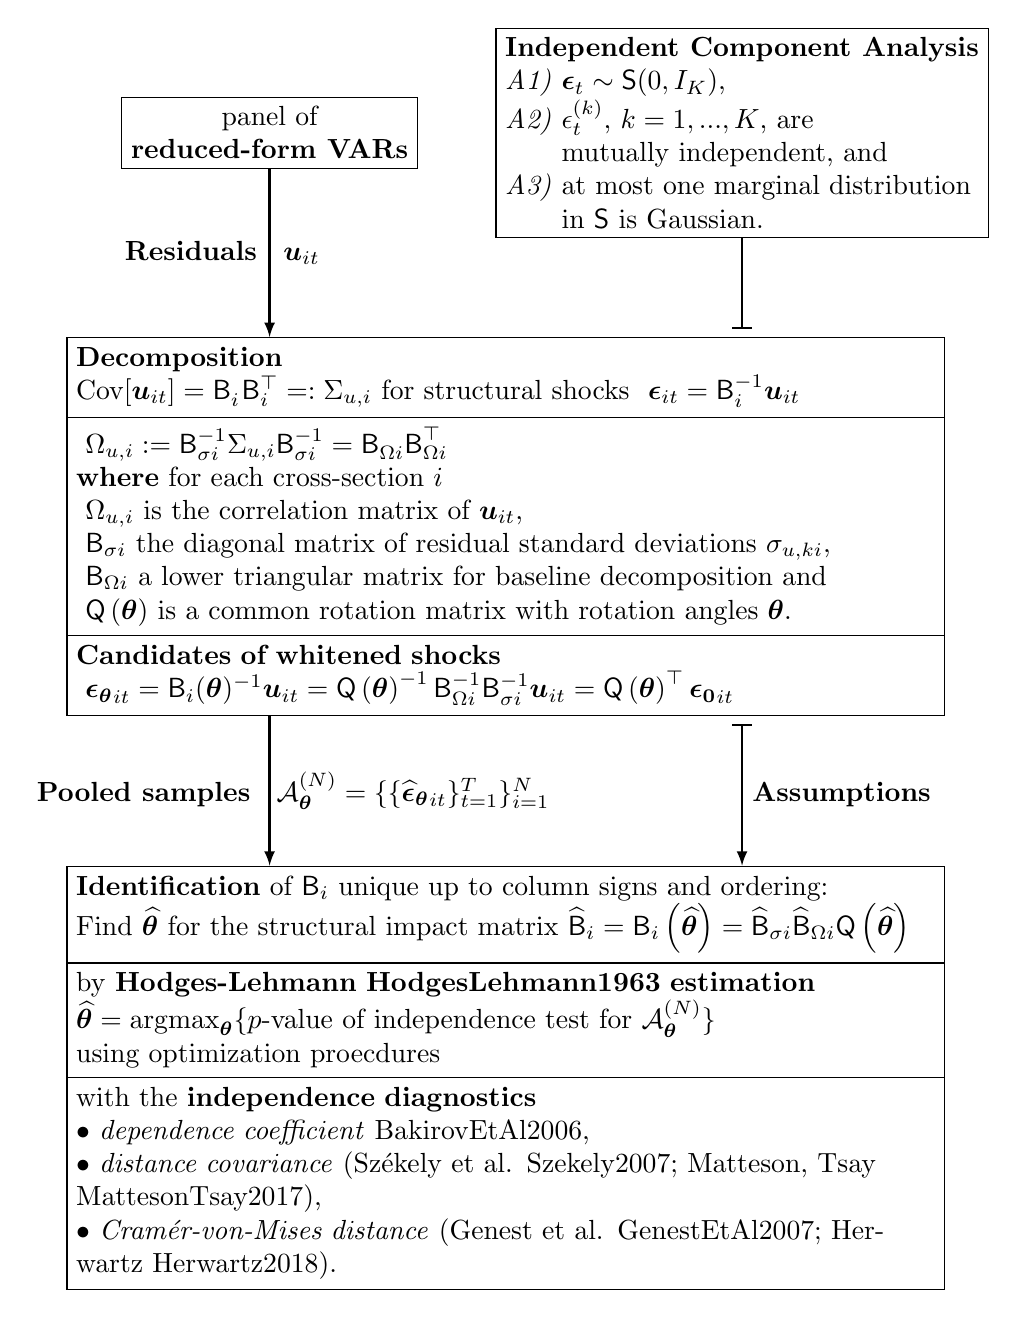
\begin{tikzpicture}
	% nodes
	\node[draw, align=center] (VAR) at ([xshift=-30mm]0,0) {
		panel of \\
		\textbf{reduced-form VARs} };
	
	\node[draw, align=left] (ICA) at ([xshift=30mm]0,0) {
		\textbf{Independent Component Analysis} \\
		\textit{A1)} $ \boldsymbol{\epsilon}_{t} \sim \mathsf{S}(0,I_K) $,  \\
		\textit{A2)} $ \epsilon_{t}^{(k)} $, $ k = 1,...,K $, are \\
		\hspace{6mm} mutually independent, and \\
		\textit{A3)} at most one marginal distribution \\
		\hspace{6mm} in $ \mathsf{S} $ is Gaussian.};
	
	\node[draw, align=left, text width=0.9\textwidth, shape=rectangle split, rectangle split parts=3] (B) at (0,-5) {
		\textbf{Decomposition} \\
		$ \text{Cov}[\boldsymbol{u}_{it}] = \mathsf{B}_i^{\ } \mathsf{B}_i^\top =: \Sigma_{u,i} $ for structural shocks $ \ \boldsymbol{\epsilon}_{it} = \mathsf{B}^{-1}_i \boldsymbol{u}_{it} $ \\
		
		\nodepart{two}
		$ \ \Omega_{u,i} := \mathsf{B}_{\sigma i}^{-1} \Sigma_{u,i} \mathsf{B}_{\sigma i}^{-1} = \textsf{B}_{\Omega i}^{\ } \textsf{B}_{\Omega i}^\top $ \\
		\textbf{where} for each cross-section $ i $ \\
		$ \ \Omega_{u,i}  $ is the correlation matrix of $ \boldsymbol{u}_{it} $, \\
		$ \ \mathsf{B}_{\sigma i} $ the diagonal matrix of residual standard deviations $ \sigma_{u,ki} $, \\
		$ \ \textsf{B}_{\Omega i} $ a lower triangular matrix for baseline decomposition and \\
		$ \ \mathsf{Q} \left( \boldsymbol{\theta} \right) $ is a common rotation matrix with rotation angles $ \boldsymbol{\theta} $.\\
		
		\nodepart{three}
		\textbf{Candidates of whitened shocks}\\
		$ \ \boldsymbol{\epsilon_\theta}_{it} = \textsf{B}_i(\boldsymbol{\theta})^{-1} \boldsymbol{u}_{it} = \mathsf{Q} \left( \boldsymbol{\theta} \right)^{-1} \textsf{B}_{\Omega i}^{-1} \mathsf{B}_{\sigma i}^{-1} \boldsymbol{u}_{it} = \mathsf{Q} \left( \boldsymbol{\theta} \right)^\top \boldsymbol{\epsilon_0}_{it} $};
	
	\node[draw, align=left, text width=0.9\textwidth, shape=rectangle split, rectangle split parts=3] (HLE) at (0,-12) {
		\textbf{Identification} of $ \mathsf{B}_i $ unique up to column signs and ordering: \\
		Find $ \boldsymbol{\widehat{\theta}} $ for the structural impact matrix $ \widehat{\mathsf{B}}_i = \mathsf{B}_i \left( \boldsymbol{\widehat{\theta}} \right) = \widehat{\mathsf{B}}_{\sigma i} \widehat{\textsf{B}}_{\Omega i} \mathsf{Q} \left( \boldsymbol{\widehat{\theta}} \right)  $ \\ %\citet[Eq.9]{Herwartz2017}
		
		\nodepart{two}
		by \textbf{Hodges-Lehmann \citeyearpar{HodgesLehmann1963} estimation} \\
		$ \boldsymbol{\widehat{\theta}} = \textrm{argmax}_{\boldsymbol{\theta}} \lbrace p\textrm{-value of independence test for } \mathcal{A}_{\boldsymbol{\theta}}^{(N)} \rbrace $ \\
		using optimization proecdures \\
		
		\nodepart{three}
		with the \textbf{independence diagnostics} \\
		$\bullet$ \textit{dependence coefficient} \citep{BakirovEtAl2006}, \\
		$\bullet$ \textit{distance covariance} (Székely et al. \citeyear{Szekely2007}; Matteson, Tsay \citeyear{MattesonTsay2017}), \\
		$\bullet$ \textit{Cramér-von-Mises distance} (Genest et al. \citeyear{GenestEtAl2007}; Herwartz \citeyear{Herwartz2018}).};
	
	% arrows
	\draw[-latex,thick] (VAR.south) -- node[xshift=-6mm] {\textbf{Residuals} \hspace{1mm} $ \boldsymbol{u}_{it} $} ([xshift=-30mm]B.north);
	\draw[-latex,thick] ([xshift=-30mm]B.south) -- node[xshift=3mm] {\textbf{Pooled samples} \hspace{1mm} $ \mathcal{A}_{\boldsymbol{\theta}}^{(N)} = \{ \{ \boldsymbol{\widehat{\epsilon}_\theta}_{it} \}^T_{t=1} \}^N_{i=1} $} ([xshift=-30mm]HLE.north);
	\draw[-|,thick] (ICA.south) -- ([xshift=30mm,yshift=1mm]B.north);
	\draw[|-latex,thick] ([xshift=30mm,yshift=-1mm]B.south) -- node[anchor=west] {\textbf{Assumptions}} ([xshift=30mm]HLE.north);
\end{tikzpicture}

}
	\label{fig:PSVAR}
\end{figure}


\textbf{Common rotation.} \citet{Herwartz2017} propose and evaluate the pooled identification procedure stylized in Figure~\ref{fig:PSVAR}. An individual decomposition $ \ \boldsymbol{\epsilon_\theta}_{it} = \mathsf{Q} \left( \boldsymbol{\theta} \right)^{-1} \textsf{B}_{\Omega i}^{-1} \mathsf{B}_{\sigma i}^{-1} \boldsymbol{u}_{it} $ allows for a common rotation $ \mathsf{Q} \left( \boldsymbol{\theta} \right) $ of the whitened shocks while accounting for heterogeneous variances and cross-variable correlations in $ \boldsymbol{u}_{it} $. Among competing \textit{pooled samples} $ \mathcal{A}_{\boldsymbol{\theta}}^{(N)} = \{ \{ \boldsymbol{\widehat{\epsilon}_\theta}_{it} \}^T_{t=1} \}^N_{i=1} $ of dimension $ K \times (T \cdot N) $, the ICA then determines the least dependent shocks $ \boldsymbol{\widehat{\epsilon}_{\widehat{\theta}}}_{it} $ with optimal $ \boldsymbol{\widehat{\theta}} $, from which $ \widehat{\mathsf{B}}_i $ is recovered for each individual.


\textbf{Common shocks.} \citet{CalhounEtAl2002} propose \textit{group ICA} and apply this to panel data originating from functional Magnetic Resonance Imaging (fMRI) of brains. In the same empirical context, \citet{RiskEtAl2014} evaluate ICA algorithms, which can be applied to the panel of reduced-form errors $ \boldsymbol{u}_{it} $ alike. Accordingly, their model $ \boldsymbol{u}_{it} = \mathsf{B}_i \boldsymbol{\epsilon}_{t} + \boldsymbol{e}_{it} $ consists of $ L $ common shocks $ \boldsymbol{\epsilon}_{t} $ and some idiosyncratic noise $ \boldsymbol{e}_{it} $ \citep[p.~227]{RiskEtAl2014}. In a two-step PCA, they firstly whiten each individual sample $ \left[\boldsymbol{\widehat{u}}_{i1}: \ldots: \boldsymbol{\widehat{u}}_{iT} \right]' = \mathsf{U}_i^{\ } \mathsf{D}_i^{\ } \mathsf{V}_i' $ by compact \textit{singular value decomposition} such that $ \mathcal{A}_i := \sqrt{T} \mathsf{U}_i' $ has an identity covariance matrix $ I_K $. They further factorize the $ T \times (K \cdot N) $ concatenated samples $ \left[ \mathcal{A}_1' : \ldots : \mathcal{A}_N' \right] = \mathsf{U} \mathsf{D} \mathsf{V}' $ and utilize the first $ L $ columns of left singular-vectors to construct a $ L \times T $ baseline sample $ \mathcal{A}_{\boldsymbol{0}}^{(2S)} := \sqrt{T} \mathsf{U}_{1:L}' $. The ICA, which becomes noise-free after this data reduction, then determines the least dependent common shocks $ \boldsymbol{\widehat{\epsilon}_{\widehat{\theta}}}_t $. The multivariate least squares regression of $ \boldsymbol{\widehat{u}}_{it} $ on $ \boldsymbol{\widehat{\epsilon}_{\widehat{\theta}}}_t $ recovers the $ K \times L $ impact matrices $ \mathsf{\widehat{B}}_i, \ \forall i=1\ldots,N $.


\textbf{ICA.} If at most one of the shocks is Gaussian, the \textit{independent component analysis} as established by \citet{Comon1994} can determine the rotation angles $ \boldsymbol{\widehat{\theta}}^{\bullet} $ and thereby identify the impact matrix $ \widehat{\mathsf{B}}_i^{\bullet} $ of the methods $ \bullet \in \lbrace (i), (N), (2S) \rbrace $. For this purpose, dependence measures $ \mathcal{D}(\cdot) $ discriminate between the candidates of whitened shocks $ \mathcal{A}_{\boldsymbol{\theta}}^{\bullet} = \mathsf{Q} \left( \boldsymbol{\theta} \right)^{-1} \mathcal{A}_{\boldsymbol{0}}^{\bullet} $ by dependencies beyond the second moment. In the spirit of Hodge-Lehmann estimation \citeyearpar{HodgesLehmann1963}, a minimization procedure $ \boldsymbol{\widehat{\theta}}^{\bullet} = \text{argmin}_{\boldsymbol{\theta}} \ \mathcal{D} \left( \mathcal{A}_{\boldsymbol{\theta}}^{\bullet} \right) $ finds the rotation angels $ \boldsymbol{\widehat{\theta}}^{\bullet} $ of the least dependent shocks. 

ICA can identify shocks and impact matrices up to to scaling, column signs, and ordering only. For example in the case of $ K=2 $, the relevant interval of a full rotation $ \theta \in (0, 2\pi] $ reduces to a quadrant, e.g.~$ \theta \in (0, \pi/2] $, since any exceeding rotation just permutes the ordering and reverses signs. If $ \theta \in (\pi/2, 2\pi] $, the results of $ \mathcal{D} \left( \mathcal{A}_{\boldsymbol{\theta}}^{\bullet} \right) $ including the minima would be identical to those of the first quadrant. Against this ambiguity, a common practice for the unique identification of $ \mathsf{B}_i $ is to \textit{(1)} choose the column ordering which maximizes the sum of the absolute diagonal elements and \textit{(2)} then switch signs of those columns whose main diagonal element turns out to be negative. Under $ \boldsymbol{\epsilon}_{it} \sim ( 0, I_K ) $, each shock is thereby attributed to the variable on which it has the strongest effect on impact.

ICA-based identification procedures for the individual SVAR are already implemented in \pkg{svars}. As we focus on their embedding into a panel framework, we just list them here briefly and refer the reader to the accompanying vignette \citep{LangeEtAl_fc} for a comprehensive overview and to the Monte Carlo study \citep{HerwartzEtAl2021} for a performance assessment. The following dependence measures $ \mathcal{D}\left( \cdot \right) $ and optimization procedures are adopted in \pkg{pvars}: The \textit{Cramér-von-Mises} (cvm) \textit{distance} by \citet{GenestEtAl2007} is used in \pkg{svars}' two-step optimization procedure with \pkg{copula} \citep{KojadinovicYan2010} and has been exemplarily applied for individual SVAR by \citet{Herwartz2018}. The \textit{distance covariance} (dCov) by \cite{Szekely2007} is used in the gradient algorithm of \pkg{steadyICA} \citep{RiskEtAl2015} and has been applied for SVAR by \citet{MattesonTsay2017}. The \textit{dependence coefficient} (dCoef) by \citet{BakirovEtAl2006} is not used in \pkg{svars} and \pkg{pvars}.\footnote{Note that dCoef and dCov are implemented in \pkg{energy} by \citet{RizzoSzekely2022}.} 




\section{Implementation} \label{sec:Implementation}
For each field of VAR application and for the supporting tools, Table~\ref{tab:pvarsDesign} displays \pkg{pvars}' core functions, the \textsf{S3}-class of their output object and their dependencies within and to other packages. In particular, several classes and their corresponding methods are imported from \pkg{svars}. In addition to the familiar methods such as \code{print()} and \code{summary()}, \pkg{pvars} offers the method \code{toLatex()} for conveniently formatting \pkg{pvars} results into Latex objects, thus minimizing the risk of reporting errors from tedious copy-pasting. 
\begin{table}[ht]	% tab:pvarsDesign
	\centering
	\caption{Package design of \pkg{pvars}.}
	\resizebox{\textwidth}{!}{
		

\begin{threeparttable}
	\begin{tabular}{llll|ll|ll}
		\hline\hline
		 & \textbf{Function} & \textbf{Class} & \textbf{Branch} & \textbf{Methods} & % for class} & %Functions for class 
		 & \textbf{Description} & \textbf{Literature}  \\ 
		\hline
		
		\multicolumn{4}{l|}{ \textbf{\ref{sec:pcoint}} Testing the cointegration rank } &  & & &  \\ 
		 & \code{pcoint.JO}   & \code{pcoint} & \code{coint.JO}  & \quad \code{print}, & & Panel \citeauthor{Johansen1988} tests & \citet{LarssonEtAl2001}, \citet{Choi2001} \\
		 & \code{pcoint.BR}   & \code{pcoint} & \code{coint.JO}  & \quad \code{summary}, & & Panel test with pooled $ \beta $  & \citet{Breitung2005} \\
		 & \code{pcoint.SL}   & \code{pcoint} & \code{coint.SL}  & \quad \code{toLatex} & & Panel SL-tests & Örsal, Droge \citeyearpar{OersalDroge2014} \\
		 & \code{pcoint.CAIN} & \code{pcoint} & \code{coint.SL}  &  & & Correlation augmented tests & Arsova, Örsal \citeyearpar{ArsovaOersal2020}, \citet{Hartung1999} \\
		 %& \code{pcoint.MSB}  & \code{pcoint} & \code{coint.MSB} & & & Panel MSB-test & Carrion-i Silvestre, Surdeanu \citeyearpar{SilvestreSurdeanu2011} \\
		 \hline
		 
		 \multicolumn{4}{l|}{ \textbf{\ref{sec:pvarx}} Estimating VAR models } & & &  & \\ 
		 & \code{pvarx.VAR} & \code{pvarx} & \code{VAR}\tnote{a)} & \quad \code{irf}, \code{print}, & & Mean-group estimation & \citet{Rebucci2010}, Pesaran, Smith \citeyearpar{PesaranSmith1995} \\
		 & \code{pvarx.VEC} & \code{pvarx} & \code{VECM} & \quad \code{summary} & & Pooled cointegrating vectors $ \beta $ & \citet{Breitung2005}, \cite{PesaranEtAl1999} \\
		 \hline
		 
		 \multicolumn{4}{l|}{ \textbf{\ref{sec:pid}} Identifying structure } & & &  & \\
		 & \code{pid.chol} & \code{pid} & \code{id.chol}\tnote{a)} & \quad \code{irf}, & & Recursive causality & \citet{Sims1980} \\ %\# \citet{Pedroni2013}
		 & \code{pid.grt} & \code{pid} & \code{id.grt}\tnote{c)} & \quad \code{print}, & & Long- \& short-run restrictions & \cite{BreitungEtAl2004} \\
		 & \code{pid.iv} & \code{pid} & \code{id.iv} & \quad \code{summary}, & & Proxy SVAR & Empting et al.~\citeyearpar{EmptingEtAl2024} \\
		 & \code{pid.dc} & \code{pid} & \code{id.dc}\tnote{a)} & \quad \code{toLatex} & & ICA by distance covariance & \quad \citet{CalhounEtAl2002} and \\
		 & \code{pid.cvm} & \code{pid} & \code{id.cvm}\tnote{a)} & & & ICA by Cramér-von-Mises dist. & \quad Herwartz, Wang \citeyearpar{Herwartz2017} \\
		 \hline
		 
		 \multicolumn{4}{l|}{ \textbf{\ref{sec:supp}} Supporting tools } & & & &  \\
		 &  \code{speci.factors} & \code{speci} & \qquad --- & \code{print} &  & Criteria for number of factors & Bai, Ng \citeyearpar{BaiNg2002,BaiNg2004}, \citet{Onatski2010} \\
		 &  \code{speci.VAR} & \code{speci} & \qquad --- & \code{print} &  & Criteria for lags $ p $ and periods $ \boldsymbol{\tau} $ & Bai, Perron \citeyearpar{BaiPerron1998,BaiPerron2003}, \citet{Yang2002} \\
		 & \code{irf\textcolor{gray}{.pvarx}} & \code{svarirf}\tnote{b)} & \code{irf\textcolor{gray}{.varx}} & \code{plot}, \code{print} & & Mean-Group IRF \textcolor{gray}{\small \textbf{[S3-METHOD]}} & \citet{Sims1980}, Gambacorta et al.~\citeyearpar{GambacortaEtAl2014} \\
		 & \code{PP.system}   & \code{svarirf}\tnote{b)} & \qquad --- & \code{plot}, \code{print} & & Persistence profiles  & \quad Lee, Pesaran \citeyearpar{LeePesaran1993} and \\
		 & \code{PP.variable} & \code{svarirf}\tnote{b)} & \qquad --- & \code{plot}, \code{print} & & (Structural) persistence profiles & \quad Pesaran, Shin \citeyearpar{PesaranShin1996} \\
		 & \code{sboot.mg} & \code{sboot}\tnote{b)} & \qquad --- &  \quad\code{print}, \code{summary}, & & Mean-group inference & Pesaran, Smith \citeyearpar{PesaranSmith1995} \\
		 & \code{sboot.pmb} & \code{sboot}\tnote{b)} & \code{sboot.mb} & \quad \code{plot}, \code{toLatex} & & Panel-block bootstrap & \citet{EmptingEtAl2024} \\% \quad \citet{EmptingEtAl2024} and \\
		 %& & & & & & Bootstrap-after-bootstrap & \quad \cite{EmptingHerwartz2021b} \\
		 \hline\hline
	\end{tabular}
	\begin{tablenotes}
		\item[a)] Consider the \proglang{R}-packages \pkg{vars} and \pkg{svars} for these functions. Like \code{id.dc}, \pkg{pvars}' \code{pid.dc} uses \pkg{steadyICA} by \citet{RiskEtAl2015}.
		\item[b)] This class and its methods are imported from the \proglang{R}-package \pkg{svars} by \cite{LangeEtAl_fc}.
		\item[c)] Its scoring algorithm is part of the \code{SVEC} function from the \proglang{R}-package \pkg{vars} by \citet{Pfaff2008a}.\\
	\end{tablenotes}
\end{threeparttable}}
	\label{tab:pvarsDesign}		
\end{table}

Figure~\ref{fig:Modules} illustrates \pkg{pvars}' modular implementation, which leads to the three layers of dependency between the library of auxiliary functions, the functions for individual econometric procedures, and their panel extensions. In this tree-like structure, the \code{aux}-functions are the hidden ``roots'' and the individual functions are ``leafy branches''. Some branches of the individual \mbox{\code{id.\hspace{-2pt}*()}} functions are a ``graftage'' from \pkg{vars} and \pkg{svars}. The individual \mbox{\code{coint.\hspace{-2pt}*()}} functions are more flexible than existing implementations of cointegration rank tests and extend the set of available specification options. Finally attached to the branches, the ``fruits'' of this package are the panel functions for each field of VAR application. These are printed in bold to emphasize their novelty and \pkg{pvars}' main contribution.
\begin{figure}[ht] % fig:Modules
	\centering
	\caption{Modular implementation in three layers.}
	\resizebox{0.75\textwidth}{!}{
		
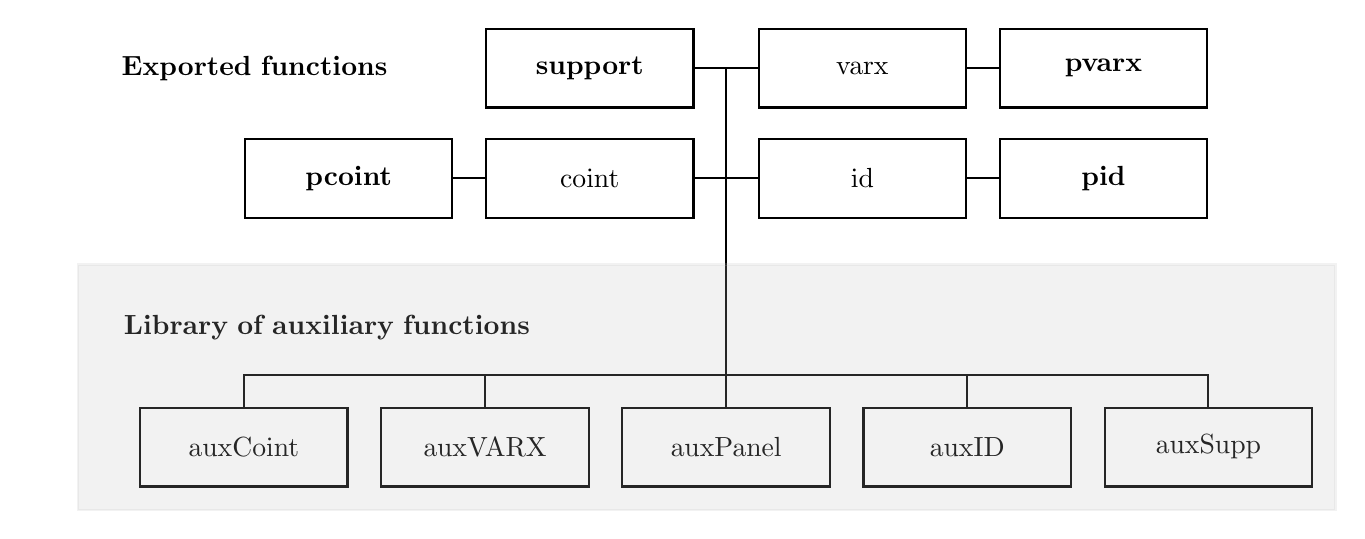
\begin{tikzpicture}[auto, node distance = 0.4cm, thick,
	every node/.style = {rectangle, black, %font = \sffamily,
		draw=black, fill=white, %top color = blue!90!black, bottom color = blue!60!black,
		text width = 2.4cm, align = center, minimum height = 1cm}]
	
	% top layer: panel functions
	\coordinate (Oben);
	\node (support) [left  = of Oben] {\textbf{support}}; %\\ \texttt{IRF} \\ \texttt{PP.system} \\ \texttt{PP.variable}};
	\node (varx)	[right = of Oben] {varx};
	\node (pvarx)	[right = of varx] {\textbf{pvarx}};
	
	% middle layer: individual functions
	\coordinate [below = 1.4cm of Oben]	(Mitte);
	\node (coint)	[left = of Mitte]	{coint};
	\node (pcoint)	[left = of coint]	{\textbf{pcoint}}; %\\ \texttt{.JO} \\ \texttt{.SL} \\ \texttt{.CAIN}};
	\node (id)		[right = of Mitte]	{id};
	\node (pid)		[right = of id]		{\textbf{pid}};
	
	% bottom layer: library of auxiliary functions
	\coordinate [below = 2.5cm of Mitte]	(Unten);
	\node (auxPanel) [below = of Unten]		{auxPanel};
	\node (auxVARX)	 [left  = of auxPanel]	{auxVARX};
	\node (auxCoint) [left  = of auxVARX]	{auxCoint};
	\node (auxID)    [right = of auxPanel]	{auxID};
	\node (auxSupp)	 [right = of auxID]	    {auxSupp};
	
	% connections
	\draw [black,thick]
	(Oben)   -- (Mitte)  -- (Unten)
	(pvarx)	 -- (varx)	 -- (Oben)  -- (support)
	(pcoint) -- (coint)  -- (Mitte) -- (id) -- (pid)
	(Unten) -| (auxVARX)
	(Unten) -| (auxCoint)
	(Unten) -| (auxPanel)
	(Unten) -| (auxID)
	(Unten) -| (auxSupp);
	
	% labels for layers 
	\node[draw=white,text width=5.5cm, above left = 0.7cm of auxCoint, anchor=south west] (Lib) {\textbf{Library of auxiliary functions}};
	\coordinate [above left  = of Lib]     (lFound);
	\coordinate [below right = of auxSupp] (rFound);
	\fill[draw=black,color=lightgray,opacity=0.2] (lFound) rectangle (rFound);
	\coordinate (pvars) at (Oben -| Lib);
	\node[draw=white,text width=5.5cm, left = 3.8cm of pvars, anchor=west] {\textbf{Exported functions}};
\end{tikzpicture}


}
	\label{fig:Modules}
\end{figure}

The idea of modular programming is to break monolithic and repetitive code down into functional sub-entities, which achieves easier maintenance, better testability, and reusability. Especially the multivariate panel procedures benefit from this kind of implementation because their functions reduce to simple re-arrangements of auxiliary functions. These can be repetitively applied over subsets of the $ K \times T \times N $ data array. Whenever sensible, the \textsf{R}-functions are vectorized in order to enable more flexible input arguments and faster matrix computation of the multivariate VAR models. In consequence, the in- and outputs are mainly matrix objects, which thereby serve as an interface between the auxiliary modules.\footnote{Note that \pkg{pvars} does not export auxiliary functions to the global environment. If the user wishes to construct own functions, she needs to call an auxiliary function \mbox{\code{pvars:::aux\_\hspace{-2pt}*()}} via a triple colon.} With automatic unit tests by \pkg{testthat} \citep{Hadley2011}, \mbox{\code{pcoint.\hspace{-2pt}*()}} and subordinated modules are checked against reproduced examples of the literature. Functions outside this hierarchy are checked against consistency with the other \pkg{vars} packages, identities derived from econometric theory, and simulation results from \citet{EmptingEtAl2024}.


\textbf{Argument structure.} In order to comply with the modular functions and their repetitive call over data subsets, several conventions have been established for the input arguments of the auxiliary, individual, and panel functions. The arguments whose names are marked with the prefix \mbox{\code{L.\hspace{-2pt}*}} are an \textsf{R}-object of class \code{list} with $ N $ elements of repeated structure. Most prominently, \code{L.data} is the panel data in \textit{list-format} and, as a repetitive \code{list}, contains $ N $ \code{data.frame}s of dimension $ T_i \times K $. In these multivariate time series, the variables must have an identical order $ k = 1, \ldots , K $ for each individual $ i = 1,\ldots,N $. All successions are binding for any other \code{L.\hspace{-2pt}*} object within the environment of a given function. Hence even in the global environment, the user should stick to a universal succession for all \code{L.\hspace{-2pt}*} objects in order to avoid confusion.

Further conventions for prefixes are \code{n.\hspace{-2pt}*} and \code{dim\_\hspace{-2pt}*}, which denote integers and refer to a quantity resp.~the dimension of a matrix or array. Straightforwardly, \code{dim\_K}, \code{dim\_T}, and \code{dim\_N} signify the data dimensions $ K $, $ T $, and $ N $ for instance. Arguments with prefix \mbox{\code{t\_\hspace{-2pt}*}} define $ \boldsymbol{\tau} $ for the period-specific deterministic regressors. As a \code{list}, they collect optional vectors of integers for trend breaks (named \code{t\_break}), shift dummies (\code{t\_shift}), and impulse dummies (\code{t\_impulse}) as well as a single integer \code{n.season}, which indicates the seasonal frequency for the centered dummies. Each integer in those vectors specifies a period $ \tau $ at which a break, shift, or impulse occurs within the interval $ 1,\ldots,T $ of the complete panel data set (i.e.~including the presamples). The following sections describe how the mandatory and optional input arguments are employed in the \pkg{pvars} functions for cointegration tests (Section~\ref{sec:pcoint}), estimation (Section~\ref{sec:pvarx}), and structural identification (Section~\ref{sec:pid}).


\subsection{Testing the cointegration rank} \label{sec:pcoint}
The panel cointegration tests are implemented in accordance with the three dimensions of panel test construction as presented in Table~\ref{tab:pcoint}. \textit{(i)} Each \code{pcoint.\hspace{-2pt}*()} function always assesses all hypotheses $ r_{H0} = 0,\ldots,K-1 $ and uses all combination approaches available for the respective underlying individual procedure. \textit{(ii)} The data generating process by contrast, which covers also the panel test generation, must be defined via the arguments of \mbox{\code{pcoint.\hspace{-2pt}*()}}. These arguments are kept consistent across the functions or refer to the underlying procedure. \textit{(iii)} The panel functions \code{pcoint.\hspace{-2pt}*()} usually loop over their internal function \code{cointf()} as the underlying procedure. \code{cointf()} arranges the auxiliary functions in the same way as its respective branch \mbox{\code{coint.\hspace{-2pt}*()}}, but has been modified for the panel test. Hence, if an individual sample does not conform with the panel result, the user may consult the individual counterpart \code{coint.\hspace{-2pt}*()} for a closer inspection of the peculiar individual entity. For this purpose, she can also consider the persistence profiles \code{PP.\hspace{-2pt}*()}. Within the scope of PANIC, the test functions \code{coint.\hspace{-2pt}*()} for the single VAR system can assess cointegration between $ \boldsymbol{F}_t $ from \eqref{eq:PANIC}, too.

\textbf{The branch of \citeauthor{Johansen1996}.} The individual Johansen procedure is available as the function
\begin{CodeChunk}
\begin{CodeInput}
coint.JO(y, dim_p, x, dim_q, type, t_D1=NULL, t_D2=NULL)
\end{CodeInput}
\end{CodeChunk}
By default, the \textsf{R} function performs both LR-test variants on the  multivariate time series \code{y} with lag order \code{dim\_p}. For the \textit{trace test} as in \eqref{eq:LRrank} and exclusively for the individual \textit{maximum eigenvalue test} with simple specifications, $p$-values are approximated by the gamma distribution. Optionally, weakly exogenous variables \code{x} with lag order \code{dim\_q} are incorporated. The character argument \code{type} defines the conventional deterministic term according to the labels for the \textit{innovative model} in Table~\ref{tab:DetTerm}. Optional breaks of the deterministic term in the periods \code{t\_D1} are treated in accordance with JMN \citeyearpar{JohansenEtAl2000} or KN \citeyearpar{KuritaNielsen2019}. The panel-extensions of the Johansen procedure are implemented by
\begin{CodeChunk}
\begin{CodeInput}
pcoint.JO(L.data, lags, type, t_D1=NULL, t_D2=NULL, n.factors=FALSE)
pcoint.BR(L.data, lags, type, t_D1=NULL, t_D2=NULL, n.iterations=FALSE)
\end{CodeInput}
\end{CodeChunk}
The input argument \code{L.data} requires a data panel in \textit{list-format} as explained above for the argument structure of \pkg{pvars} functions in general. \code{lags} defines the lag order $ p_i $ of the individual VAR models in levels and is either a vector of $ N $ integers or a single integer for a common lag order $ p=p_i $. For assigning the heterogeneous lag orders to each individual, the integers $ p_i $ must have the same succession  $ i = 1, \ldots , N $ as \code{L.data}. The optional argument \code{n.factors} can activate the PANIC-defactoring, where the common components with the chosen number of factors $ \boldsymbol{F}_t $ are subtracted. Then, the idiosyncratic cointegration rank tests are fixed to the distribution moments for \textit{SL\_trend} irrespective of the specification of \code{type}. Specifically \code{pcoint.BR()} uses the LM-test from \eqref{eq:LMrank} instead, where \code{n.iterations} defines the number of repetition in the two-step estimation of $ \beta_{K} $. Note that any deterministic term is equipped with a heterogeneous effect $ \beta_{0i} $ in order comply with the Brownian bridges in the individual $ Z_{r\perp} $. The corresponding option \code{idx\_pool} in \code{pvarx.VEC()} is thus disabled in  \code{pcoint.BR()} and just cancels out.


\textbf{The branch of \citeauthor{SaikkonenLutkepohl2000}.} The individual SL-procedure is available via
\begin{CodeChunk}
\begin{CodeInput}
coint.SL(y, dim_p, type_SL, t_D=NULL)
\end{CodeInput}
\end{CodeChunk}
The arguments therein are the same as in the individual Johansen procedure except for \code{type\_SL}, which requires a label for the \textit{additive model} from Table~\ref{tab:DetTerm}. Optional breaks of the deterministic trend in the periods  \code{t\_D} are treated in accordance with TSL \citeyearpar{TrenklerEtAl2008}. The panel-extensions of the SL procedure are implemented by
\begin{CodeChunk}
\begin{CodeInput}
pcoint.SL(L.data,   lags, type="SL_trend", t_D=NULL, n.factors=FALSE)
pcoint.CAIN(L.data, lags, type="SL_trend", t_D=NULL)
\end{CodeInput}
\end{CodeChunk}
Again, the specifications of the input arguments are identical to those of the Johansen procedure \code{pcoint.JO} except for the \code{type} of the additive model. The default is \code{"SL\_trend"} as \citet{OersalDroge2014} propose for their panel SL-test, \citet{ArsovaOersal2020} for the CAIN-test, and \citeauthor{ArsovaOersal2017} \citeyearpar{ArsovaOersal2017,ArsovaOersal2018} enforce after the defactoring in PANIC.


\subsection{Estimating VAR models} \label{sec:pvarx}
The position of the individual VAR model of \eqref{eq:VAR} as the basic econometric unit of Section~\ref{sec:Review} is reflected in the \textsf{R}-implementation by its class \code{varx}. Accordingly, \textit{(i)} panel VAR estimates of class \code{pvarx} contain a repeated list \code{L.varx} of individual VAR, \textit{(ii)} SVAR estimates \code{id} inherit from the parent class \code{varx}, and \textit{(iii)} panel SVAR estimates \code{pid} define their \code{L.varx} as a list of individual \code{id} objects. Hence, each individual VAR embedded in the panel estimates can be separately inspected by the methods for \code{varx} objects.

In \pkg{pvars}, \code{varx} also serves as an intermediary class to ensure compatibility to the other packages of the \pkg{vars}-ecosystem. Either estimated via \pkg{pvars}' \code{VECM()} or coerced from \pkg{vars}' \code{varest} and \code{vec2var} objects via \code{as.varx()}, the \code{varx} objects can then enter the same functions since the class obeys a unifying construction plan for different VAR model types. If the user wishes to employ \pkg{pvars} function to VAR objects of other classes, she may simply specify accordant \code{as.varx()}-methods instead of altering the original \pkg{pvars} function. 
A list of class \code{varx} contains the coefficient matrix \code{\$A} for the \textit{full-system} and \textit{level-representation} of the VAR model, its residual covariance matrix \code{\$SIGMA}, and a structural impact matrix \code{\$B}. In reduced-form VAR objects, the latter is just a placeholder \code{\$B} $ = I_K $ such that \code{irf()} generates \textit{forecast-error impulse responses} \cite[p.~52]{Lutkepohl2005}. In SVAR object of class \code{id}, \code{\$B} is the result of an identification procedure. If a cointegration rank-restriction or conditional estimation is employed, the estimates and specifications of these VAR representations are stored in the slots \code{\$VECM}, \code{\$PARTIAL}, and \code{\$MARGINAL} and then transformed to the top-level \code{\$A}.


\textbf{Panel of VAR models.} Extended from the branch of individual VAR resp.~VECM, the estimators for the VAR models of heterogeneous panels
\begin{CodeChunk}
\begin{CodeInput}
pvarx.VAR(L.data, lags, type, t_D=NULL, D=NULL)
pvarx.VEC(L.data, lags, dim_r, type, t_D1=NULL, t_D2=NULL, 
          D1=NULL, D2=NULL, idx_pool=FALSE, n.iterations=FALSE)
\end{CodeInput}
\end{CodeChunk}
use data panels in list-format \code{L.data} to estimate a list of individual VAR models \code{\$L.varx}. The specifications of the VAR processes are the lag orders \code{lags}, the \code{type} of the conventional deterministic term, and optional deterministic regressors activated in the periods \code{t\_D} resp.~\code{t\_D1} and \code{t\_D2}. While these arguments of \code{pvarx.VEC()} comply with the labels in Table~\ref{tab:DetTerm} and with $ \boldsymbol{d}_{1t} $ and $ \boldsymbol{d}_{2t} $ in \eqref{eq:VECM}, \code{pvarx.VAR()} is in accord with \pkg{vars}' well-known \code{VAR()} function and accepts a \code{"const"}, a linear \code{"trend"}, \code{"both"}, or \code{"none"} in $ \boldsymbol{d}_{t} $ of each individual model in \eqref{eq:VAR}. Customized regressors can be included as a common single data matrix or a \code{list} of individual data matrices (including the presample) via \code{D} in VAR models and via restricted \code{D1} and unrestricted \code{D2} in VECM. Unlike \code{t\_D}, \code{t\_D1}, and \code{t\_D2}, these arguments do not add accompanying lagged regressors to $ \boldsymbol{d}_{2t} $ automatically.
 
In the next step, the individual coefficients are combined by cross-sectional averages. This provides \textit{(i)} Pesaran and Smith's \citeyearpar{PesaranSmith1995} mean-group (MG) estimation as suggested by \citet{CanovaCiccarelli2013} and assessed by \citet{Rebucci2010} for VAR or \textit{(ii)} Pesaran et al.'s  \citeyearpar{PesaranEtAl1999} pooled mean-group (PMG) estimation if Breitung's \citeyearpar{Breitung2005} two-step estimator has been selected. The latter is activated if some variables \code{idx\_pool} are restricted to have homogeneous coefficients in the \code{dim\_r} cointegrating vectors \code{\$beta}. For this, the  switching algorithm can be used with further \code{n.iterations}. If all elements of \code{idx\_pool} are in $ \left[0, \ldots , r \right] $, the coefficients up to the uniform upper block $ I_{r} $ are throughout heterogeneous and estimated with the individual estimator by \citet{AhnReisel1990}. All resulting panel estimates such as \code{\$A} or \code{\$beta} are stored in top-level slots of the \code{pvarx} objects. 



\subsection{Identifying structure} \label{sec:pid}
Equivalently to \pkg{svars}' \code{id.\hspace{-2pt}*()} procedures for individual VAR objects, \pkg{pvars}' \code{pid.\hspace{-2pt}*()} functions are applied to \code{pvarx} objects containing the panel estimates of the reduced-form VAR. Accordingly, the arguments to control the underlying identification procedures are identical to those of the \pkg{svars} package. \cite{LangeEtAl_fc} describe the implementation and application of the identification procedures in detail. 


\textbf{Imposed.} Theoretical considerations like recursive causality may imply restrictions which can be imposed uniformly on $ \mathsf{{B}_i} $ of each individual VAR model. Some ensuing functions of Section~\ref{sec:supp} accept a simple list of individual \pkg{svars} objects, too, which will produce identical results under these restrictions. However, to enable the full functionality of the \pkg{pvars} package, the following functions are added as panel equivalents into the \code{pid.\hspace{-2pt}*()} canon. 
\begin{CodeChunk}
\begin{CodeInput}
pid.chol(x, order_k=NULL)
pid.grt(x, LR=NULL, SR=NULL, start=NULL, max.iter=100, conv.crit=1e-07, maxls=1.0)
\end{CodeInput}
\end{CodeChunk}
The function \code{pid.chol()} is the direct extension of \pkg{svars}' \code{id.chol()}, where the optional argument \code{order\_k} allows for specifying alternative causal orderings in the Cholesky decomposition. The panel function \code{pid.grt()} and its individual counterpart perform the ML estimation of \eqref{eq:svecmLikeli} for SVECM under short and long-run restrictions on the $ K \times K $ matrices \code{SR} resp.~\code{LR}. Using the scoring algorithm from \pkg{vars}' \code{SVEC()}, they have identical arguments to tune the optimization procedure as \citet[Sec.~3.2]{Pfaff2008a} describes in detail.\footnote{This function integrates \pkg{vars}' \code{SVEC()} into the \pkg{pvars} system on the panel level. \code{SVEC()} cannot be applied to objects of class \code{cajo-test}, i.e.~\pkg{urca}'s VECM object with restricted $ \alpha $ or $ \beta $, although these restrictions contribute to the identification of structural shocks. As an individual counterpart, \code{id.grt()} is applied to \code{varx} objects, allowing for complex deterministic terms, the MB bootstrap, and \code{svarirf} methods.} If the input object \code{x} contains pooled cointegrating coefficients $ \beta_k=\beta_{ki} $, those are used to calculate the orthogonal complement $ \beta_{\perp} $ in the structural identification of \eqref{eq:GRT}.


\textbf{Data-driven.} Residual structure in $ \boldsymbol{u}_{it} $ such as non-Gaussianity allows data-driven identification. For this purpose, \pkg{pvars} offers the panel applications of ICA. Via the argument \code{combine}, the user can select a strictly individual identification of $ \textsf{B}_i $ as in \pkg{svars} (using \code{"indiv"}), a common rotation of pooled shocks by \citet{Herwartz2017} (\code{"pool"}), or \code{n.factors} common shocks across the individuals by \citet{CalhounEtAl2002} (\code{"group"}). 
\begin{CodeChunk}
\begin{CodeInput}
pid.dc(x,  combine, n.factors=NULL, n.iterations=100, PIT=FALSE)
pid.cvm(x, combine, n.factors=NULL, dd=NULL, itermax=500, steptol=100, iter2=75)
\end{CodeInput}
\end{CodeChunk}
The panel identification functions pass the combined samples of whitened shocks to the ICA procedures. Like \code{id.dc()} in \pkg{svars}, \code{pid.dc()} uses the gradient algorithm from \pkg{steadyICA} to minimize the distance covariance (dCov) with respect to the rotation angles $ \boldsymbol{\theta} $. Their joint option \code{PIT} activates \textit{probability integral transformation}, which transforms the marginal densities of the structural shocks before evaluating dCov. The maximum number of iterations is \code{n.iterations=100} by default. The panel function \code{pid.cvm()} uses the procedure from \pkg{svars}' \code{id.cvm()} to minimize the CvM distance. For both CvM functions, \pkg{copula}'s \citep{KojadinovicYan2010} \code{indepTestSim()} simulates the distribution of test statistics under independence, which is either provided via \code{dd} or called internally if \code{dd=NULL}. The external provision of \code{dd} saves computation time if simulated once and then used for multiple calls of \code{id.cvm()} or \code{pid.cvm()} on \code{x} with identical sample dimensions. The remaining arguments control the two-step optimization procedure for $ \boldsymbol{\widehat{\theta}} $. In a first step, the differential evolution algorithm from \pkg{DEoptim} \citep{MullenEtAl2011} determines preliminary angles $ \boldsymbol{{\theta}^*} $ within \code{itermax} iterations under a tolerance of \code{steptol}. The second step further optimizes the test statistic in \code{iter2} iterations locally around $ \boldsymbol{{\theta}^*} $.

All \mbox{\code{pid.\hspace{-2pt}*()}} functions extend their \code{pvarx} input to the class \code{pid}. Therein, the structural impact matrices $ \mathsf{\widehat{B}_i} $ have been assigned to each SVAR object in \code{\$L.varx} and their mean-group estimates to the top-level slot \code{\$B} next to \code{\$A}. By default, the ICA-based panel functions order the columns of all $ \mathsf{\widehat{B}_i} $ uniformly pursuant to the aforementioned convention of the SVAR literature. Consequently, the main diagonal of the mean-group \code{\$B} holds the maximum absolute estimates as positive coefficients $ \mathsf{\widehat{b}}_{kk} $. Mean-group statistics of $ \widehat{\mathsf{B}}_i $ as presented in \citet{BernothHerwartz2021} and \citet{Herwartz2017} can be viewed via \code{pid}'s \code{summary()} method and exported via \code{toLatex()}.


\subsection{Supporting tools} \label{sec:supp}
\textbf{Dynamic analysis.} In the \pkg{vars}-ecosystem, several tools of dynamic analysis are already available such as \textit{impulse response functions} (IRF), \textit{forecast error variance decomposition} (FEVD) and \textit{historical decomposition} (HD). \pkg{pvars} extends this list by \textit{mean-group IRF} \citep[p.~627]{GambacortaEtAl2014}. Given a VAR object \code{x} of class \code{pvarx} or \code{pid}, the method 
\begin{CodeChunk}
\begin{CodeInput}
irf(x, n.ahead=20, normf=NULL, w=NULL)
\end{CodeInput}
\end{CodeChunk}
calculates the cross-sectional average of individual responses for each period after the initial impulse. The function optionally provided in \code{normf} normalizes the shock size of these impulses. Vector \code{w} with names, $ N $ logical, or $ N $ numeric elements allows to select a subset of the $ N $ individuals resp.~to apply real-valued weights in the mean-group estimation.


\textit{Persistence profiles} (PP) by \citet{PesaranShin1996} are particularly useful for panel cointegration analysis. Given an individual VECM, they map the speed of convergence to the long-run equilibrium after an impulse shock and thus allow to counter-check the individual error correction behavior under a common cointegration rank or pooled cointegration matrix. While a reversion to the $r$ long-run equilibria is the defining property of cointegration, explosive roots can emerge from ignored breaks in the deterministic term on the individual level and contaminate the panel results. In \pkg{pvars}, the functions 
\begin{CodeChunk}
\begin{CodeInput}
PP.system(x,   n.ahead=20)
PP.variable(x, n.ahead=20, shock=NULL)
\end{CodeInput}
\end{CodeChunk}
calculate PP initiated by \textit{system-wide shocks} resp.~by \textit{variable-specific shocks} based on the Cholesky decomposition of $ \widehat{\Sigma}_{u,i} $. \textit{Structural shocks} are derived from $ \widehat{\mathsf{B}}_i $ if \code{x} is a structural VECM object of class \code{id} instead of the reduced-form \code{varx}. The matrix \code{shock} controls via its $K$ rows which shocks are selected and combined. Both tools, \code{PP.*()} and \code{irf()}, return \code{svarirf} objects, for which \pkg{svars} provides the \code{plot} method to visualize the responses over a horizon of up to \code{n.ahead} time periods.


\textbf{Bootstrapping.} Bootstrap procedures are a standard tool for VAR modeling to reconstruct the sampling distribution and perform inference. For estimating standard errors of point estimates and confidence bands of structural impulse-responses, \pkg{pvars} provides recursive-design bootstrap procedures. In particular, the following functions implement the moving-block bootstrap for individual VAR models \citep{BruggemannEtAl2016} and the panel-block bootstrap \citep{EmptingEtAl2024} respectively. 
\begin{CodeChunk}
\begin{CodeInput}
sboot.mb(x, b.length=1, n.ahead=20, n.boot=500, n.cores=1, 
	  deltas=cumprod((100:0)/100), normf=NULL)
sboot.pmb(x, b.dim=c(1, 1), n.ahead=20, n.boot=500, n.cores=1, 
	  deltas=cumprod((100:0)/100), normf=NULL, w=NULL)
\end{CodeInput}
\end{CodeChunk}
Given an estimated (panel) SVAR object \code{x} of class \code{id} reps.~\code{pid}, the bootstrap functions iterate \code{n.boot} times re-estimating the VAR models, their structural matrices $ \mathsf{B}_i $, and impulse responses over a horizon of up to \code{n.ahead} periods. The arguments from the SVAR object itself (i.e.~model specifications, estimation and identification methods, optional restrictions on $ \alpha_i \beta^\top $ like rank and weak exogeneity) are passed to and fixed over the bootstrap iterations. In order to speed up their computation by parallel processing, more than one CPU core can be assigned to the procedure via \code{n.cores}. The resulting \pkg{svars} object of class \code{sboot} allows to plot IRF confidence bands via \pkg{svars}' \code{plot()} method. Confidence intervals for parameters $ A $ or $ \mathsf{B} $ can be viewed via \code{summary()} and exported via \code{toLatex()}.

If input \code{x} contains bias-correction terms \code{PSI\_bc} resp.~\code{L.PSI\_bc}, both functions perform a bias-corrected bootstrap. For example, objects from a first bootstrap contain such terms and thus enable the bootstrap-after-bootstrap of individual \citep{Kilian1998} or panel VAR models \citep{EmptingEtAl2024}, where the weights \code{deltas} control a successive stationarity correction. \code{plot()} then displays small-sample corrected IRF and their confidence bands. 

The argument \code{b.dim} defines the dimensions $ \left( b_{(t)}, b_{(i)} \right) $ of the panel blocks for temporal and cross-sectional resampling. The default \code{c(1, 1)} specifies an \textit{iid.}~resampling in both dimensions, \code{c(1, FALSE)} a temporal resampling, and \code{c(FALSE, 1)} a cross-sectional resampling. Choosing integers $ b_{(t)}, \ b_{(i)} > 1 $ assembles blocks of consecutive residuals to capture residual structure like ARCH or cross-sectional correlation. Moreover, \code{sboot.mb()} complements \pkg{svars}' \code{mb.boot()} \citep[Sec.~3.6 and 4.2]{LangeEtAl_fc} and accepts individual SVAR objects identified by \code{id.grt()} \citep{BreitungEtAl2004} or \code{id.iv()} \citep{JentschLunsford2021}. Here, the default \code{b.length=1} implies the residual \textit{iid.}~bootstrap as implemented in \pkg{vars}' \code{irf()}, while a single integer $ b_{(t)} > 1 $ defines the length of temporal blocks for a moving-block bootstrap.




\section{Empirical illustrations} \label{sec:Illustration}
Several empirical illustrations accompany the package to demonstrate its application. 
In the \code{help()} for functions, the examples provide chunks of \proglang{R}-code for directly copy-pasting unit-tested reproductions. 
In this section, we focus on the workflow of \pkg{pvars} and therefore guide the user to first organize the $ K \times T \times N  $ data array, then perform a panel cointegration analysis, and finally export the results to Latex. Specifically, the reproduced example of \citet{ArsovaOersal2017} in Section~\ref{sec:MERM} illustrates how to perform the \textit{Panel Analysis of Nonstationarity in Idiosyncratic and Common components} (PANIC), and the reproduced example of \citet{ArsovaOersal2020} in Section~\ref{sec:ERPT} how to specify deterministic terms. The \proglang{R}-code for both illustrations is assembled in the file \textit{pvars\_reproductions.R} in \pkg{pvars}' \textit{examples} folder. 
A comprehensive illustration can be found in \citet{EmptingHerwartz2021b}, who go through the pretests and VAR-applications \ref{sec:pcoint} to \ref{sec:supp} successively.


\textbf{Data format.} The exemplary data sets of the \pkg{pvars} package are panels in the popular \textit{long-format}, where all $ N $ multivariate time series have been transposed into $ T \times K $ matrices and stacked into an $ (N \cdot T) \times (2 + K)  $ \code{data.frame} object. The two additional columns \code{id\_i} and \code{id\_t} contain \code{factor} elements, which serve as identifiers for individual $ i $ and time period $ t $. Accordingly, each observation $ \boldsymbol{y}_{it} $ is stored in a single row. The \code{factor} variables preserve the predefined \code{levels} order $ 1,\ldots,N $ within the complete long-format data panel or its subsets.\footnote{Thereby, we also preempt the data management of \proglang{R} versions older than release 4.0.0, which would coerce \code{character} vectors into \code{factor} columns automatically and sort their \code{levels} alphabetically. For instance, this could lead to mismatches when switching between label standards as in the case of Switzerland with the ISO-3166 abbreviation ``CHE''.} In the following, we consider the data set \code{MERM} and firstly extract the names of the variables $ k = 1, \ldots, K $ and countries $ i = 1, \ldots, N $.
\begin{CodeChunk}
\begin{CodeInput}
R> library("pvars")
R> data("MERM")
R> names_k = colnames(MERM)[-(1:2)]
R> names_i = levels(MERM$id_i)
R> head(MERM, n=3)
\end{CodeInput}
\begin{CodeOutput}
    id_i     id_t          s         m          y         p
1 Brazil 1995_Jan -0.1660546 -3.094546 0.07401953 0.3357538
2 Brazil 1995_Feb -0.1731636 -3.054644 0.07127137 0.3422039
3 Brazil 1995_Mar -0.1176580 -3.055017 0.06986985 0.3539417
\end{CodeOutput}
\end{CodeChunk}
Naturally, \pkg{pvars}' modular implementation works well with panel data in \textit{list-format}, where each of the $ N $ listed elements is an individual matrix of $ T \times K $ time series. This can be constructed by either writing separate time series into the \code{list} object or transforming the long-format\footnote{\textit{Wide-format} panels may be transformed into long-format first. The function \code{melt()} of the \pkg{reshape2} package \citep{Hadley2007} can perform this task. Consider his vignette for a more detailed explanation of these two data formats and for an additional, third way to transform data into list-format.} data panel via  \code{sapply()}.
\begin{CodeChunk}
\begin{CodeInput}
R> L.data = sapply(names_i, FUN=function(i) 
+     ts(MERM[MERM$id_i==i, names_k], start=c(1995, 1), frequency=12), 
+     simplify=FALSE)
\end{CodeInput}
\end{CodeChunk}
Here, the individual matrices in \code{L.data} have been defined as time series objects \code{ts} with \code{frequency=12} for monthly observations starting in January 1995. Although the functions in \pkg{pvars} do not require this, the \code{ts}-definition simplifies the workflow when using further packages like \pkg{ggplot} \citep{Wickham2016}. The panel functions yet resort to the names of the listed time series as labels for individual results. \code{sapply()} assigns this definition directly, but \code{names()} can enforce this subsequently, too, as an alternative transformation requires:
\begin{CodeChunk}
\begin{CodeInput}
R> L.data = lapply(names_i, FUN=function(i) MERM[MERM$id_i==i, names_k]) 
R> names(L.data) = names_i
\end{CodeInput}
\end{CodeChunk}
Either way, the data set is now readily prepared for the econometric analysis with \pkg{pvars}.


\subsection{The monetary exchange rate model: Conduct a PANIC} \label{sec:MERM}
\cite{ArsovaOersal2017} illustrate the PANIC analysis of the \textit{monetary exchange rate model} (MERM), according to which the nominal exchange rate $ s_{it} $ between two countries forms a long-run relationship with their relative level of money supply and their relative level of output. As \citet{Dabrowski2014} propose, \citeauthor{ArsovaOersal2017} adopt the log-linear model 
\begin{align} \label{eq:MERM}
\begin{split}
	s_{it} & = \mu_{0i} + \mu_{1i} t + \beta_{i1} \left( m_{it} - m^*_{t} \right) + \beta_{i2} \left( y_{it} - y^*_{t} \right) + \beta_{i3} \left[ \left( p_{it} - p^T_{it} \right) - \left( p^*_{t} - p^{T*}_{t} \right) \right] + u_{it},
\end{split}
\end{align}
where the variables for the USA as the preselected reference country are marked with an asterisk. The natural logarithm of the dollar exchange rate for a country $ i $ is denoted by $ s_{it} $, the logarithmized nominal money supply by $  m_{it} $, and the logarithmized industrial production index by $  y_{it} $. Moreover, they have included the natural logarithm of consumer price index $ p_{it} $ and producer price index $ p^T_{it} $ for country $ i $ and likewise for the USA. 


\textbf{Data.} As \code{head(MERM)} has shown for the illustrative transformation of the data format, the data set \code{MERM} contains $ K=4 $ variables. These already summarize each log-ratio of Model~\eqref{eq:MERM} and thus enter the additive Model~\eqref{eq:PANIC} directly as the observed time series $ \boldsymbol{y}_{it} $. The  monthly observations cover the period $ 1995/01 - 2007/12 $ $ (T = 156) $ for $ N = 19 $ countries and are listed in \code{L.data} after transforming their data format. The names of \code{L.data}'s $ 19 $ elements provide the labels for the ``individuals'' in Table~\ref{tab:MERM}.


\textbf{Approximate factor model.} The first step of PANIC is to estimate the approximate factor model in Eq.~\eqref{eq:PANIC}, which splits $ \boldsymbol{y}_{it} $ into common and idiosyncratic components $ \Lambda_i' \boldsymbol{F}_t $ resp. $ \boldsymbol{y}^{i \! d}_{it} $. The factor model considers the data panel just as a collection of time series without individual structure. Both dimensions $ T \times NK $ of the data are assumed to be large and both components of the model may involve mixes of $  I(0) $ and $ I(1) $ series. First-differencing these data panels beforehand is a valid choice to estimate the factor model by PCA \citep{BaiNg2004} and to determine its number of common factors $ \boldsymbol{F}_t $ by the eigenvalues.\footnote{See \cite{CoronaEtAl2017} for an overview and Monte Carlo results. An exception is the set of $ IPC(k) $ criteria by \citet{Bai2004}, who seek to distinguish non-stationary factors from stationary idiosyncratic series. Accordingly, \code{speci.factors()} suppresses their result if \code{differenced=TRUE} is selected.} The information criteria in \code{[[1]]} however ignore the individual structure of our panel and thus tend to pick up the domestic dependencies between the $ K=4 $ variables within countries. Since we are interested in the factors describing cross-sectional dependence only, we prefer the specification procedure by \cite{Onatski2010}. His \textit{edge distribution} \code{ED}\footnote{\pkg{phtt} by \citet{BadaLiebl2014} with \code{OptDim(obj, criteria="ED")} has been removed from CRAN.} is more robust against domestic dependencies because it looks for a characteristic kink in the ordered eigenvalues. \code{ED} also works with the original \code{L.data} in levels irrespective of the components' order of integration. In order to find the optimal number of factors within the discrete interval $ \lbrace 0,\ldots,20 \rbrace $, we enter the \proglang{R} function 
\begin{CodeChunk}
\begin{CodeInput}
R> speci.factors(L.data, k_max=20, n.iterations=4)
\end{CodeInput}
\begin{CodeOutput}
### Optimal number of common factors ###
[[1]]
   PC IC IPC
p1 20 20   7
p2 20 20   7
p3 20 20   5

[[2]]
ER GR ED 
1  2  8 
\end{CodeOutput}
\end{CodeChunk}
A numerical result for \code{ED} indicates that the default of \code{n.iterations=4} allows Onatski's \citeyearpar{Onatski2010} edge distribution to converge. In case of an \code{NA}, the user needs to increase the number of iterations, but small numbers are often sufficient. 

The result of eight common factors can be visualized and checked in a scree plot. In accordance with PANIC of the \code{pcoint} functions, we may consider the factor model estimated with the first-differenced and standardized data now: 
\begin{CodeChunk}
\begin{CodeInput}	
R> R.fac0 = speci.factors(L.data, k_max=20, n.iterations=4, 
+    differenced=TRUE, centered=TRUE, scaled=TRUE, n.factors=8)

R> library("ggplot2")
R> pal = c("#999999", RColorBrewer::brewer.pal(n=8, name="Spectral"))
R> lvl = levels(R.fac0$eigenvals$scree)
R> ggplot(R.fac0$eigenvals[1:20, ]) +
+    geom_col(aes(x=n, y=share, fill=scree), color="black", width=0.75) +
+    scale_fill_manual(values=pal, breaks=lvl, guide="none") +
+    labs(x="Component number", y="Share on total variance", title=NULL) +
+    theme_bw()
\end{CodeInput}
\end{CodeChunk}
\begin{figure}[ht] % fig:Scree
	\centering
	\caption{Scree plot.}
	\resizebox{0.8\textwidth}{!}{
		% Created by tikzDevice version 0.12.3.1 on 2021-03-02 17:23:06
% !TEX encoding = UTF-8 Unicode
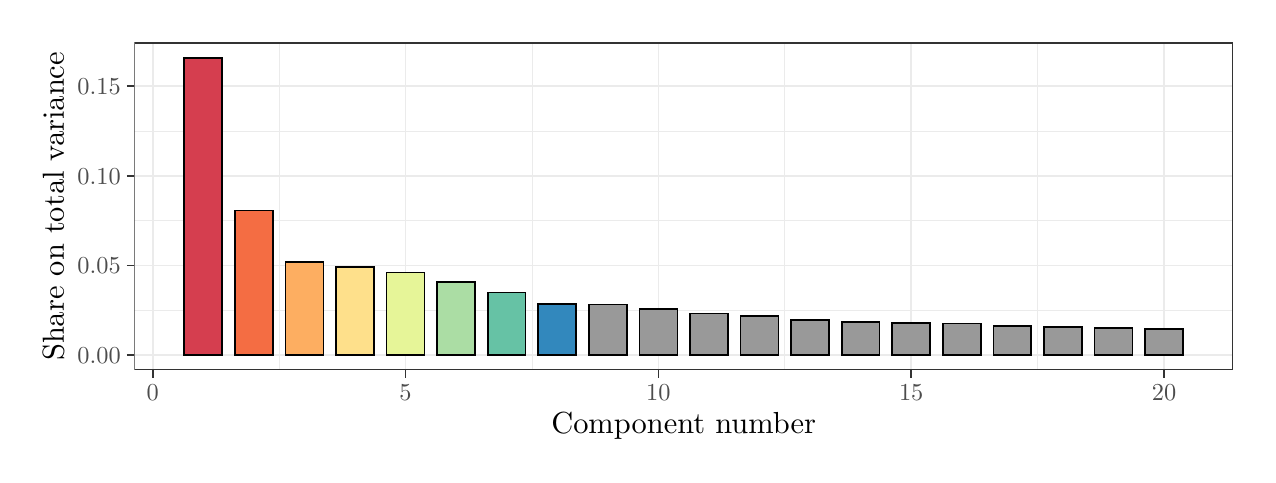
\begin{tikzpicture}[x=1pt,y=1pt]
\definecolor{fillColor}{RGB}{255,255,255}
\path[use as bounding box,fill=fillColor,fill opacity=0.00] (0,0) rectangle (441.02,154.36);
\begin{scope}
\path[clip] (  0.00,  0.00) rectangle (441.02,154.36);
\definecolor{drawColor}{RGB}{255,255,255}
\definecolor{fillColor}{RGB}{255,255,255}

\path[draw=drawColor,line width= 0.6pt,line join=round,line cap=round,fill=fillColor] (  0.00,  0.00) rectangle (441.02,154.36);
\end{scope}
\begin{scope}
\path[clip] ( 38.56, 30.69) rectangle (435.52,148.86);
\definecolor{fillColor}{RGB}{255,255,255}

\path[fill=fillColor] ( 38.56, 30.69) rectangle (435.52,148.86);
\definecolor{drawColor}{gray}{0.92}

\path[draw=drawColor,line width= 0.3pt,line join=round] ( 38.56, 52.24) --
	(435.52, 52.24);

\path[draw=drawColor,line width= 0.3pt,line join=round] ( 38.56, 84.61) --
	(435.52, 84.61);

\path[draw=drawColor,line width= 0.3pt,line join=round] ( 38.56,116.98) --
	(435.52,116.98);

\path[draw=drawColor,line width= 0.3pt,line join=round] ( 90.86, 30.69) --
	( 90.86,148.86);

\path[draw=drawColor,line width= 0.3pt,line join=round] (182.22, 30.69) --
	(182.22,148.86);

\path[draw=drawColor,line width= 0.3pt,line join=round] (273.58, 30.69) --
	(273.58,148.86);

\path[draw=drawColor,line width= 0.3pt,line join=round] (364.94, 30.69) --
	(364.94,148.86);

\path[draw=drawColor,line width= 0.6pt,line join=round] ( 38.56, 36.06) --
	(435.52, 36.06);

\path[draw=drawColor,line width= 0.6pt,line join=round] ( 38.56, 68.43) --
	(435.52, 68.43);

\path[draw=drawColor,line width= 0.6pt,line join=round] ( 38.56,100.80) --
	(435.52,100.80);

\path[draw=drawColor,line width= 0.6pt,line join=round] ( 38.56,133.17) --
	(435.52,133.17);

\path[draw=drawColor,line width= 0.6pt,line join=round] ( 45.18, 30.69) --
	( 45.18,148.86);

\path[draw=drawColor,line width= 0.6pt,line join=round] (136.54, 30.69) --
	(136.54,148.86);

\path[draw=drawColor,line width= 0.6pt,line join=round] (227.90, 30.69) --
	(227.90,148.86);

\path[draw=drawColor,line width= 0.6pt,line join=round] (319.26, 30.69) --
	(319.26,148.86);

\path[draw=drawColor,line width= 0.6pt,line join=round] (410.62, 30.69) --
	(410.62,148.86);
\definecolor{drawColor}{RGB}{0,0,0}
\definecolor{fillColor}{RGB}{213,62,79}

\path[draw=drawColor,line width= 0.6pt,line cap=rect,fill=fillColor] ( 56.60, 36.06) rectangle ( 70.30,143.48);
\definecolor{fillColor}{RGB}{244,109,67}

\path[draw=drawColor,line width= 0.6pt,line cap=rect,fill=fillColor] ( 74.87, 36.06) rectangle ( 88.58, 88.35);
\definecolor{fillColor}{RGB}{253,174,97}

\path[draw=drawColor,line width= 0.6pt,line cap=rect,fill=fillColor] ( 93.14, 36.06) rectangle (106.85, 69.74);
\definecolor{fillColor}{RGB}{254,224,139}

\path[draw=drawColor,line width= 0.6pt,line cap=rect,fill=fillColor] (111.42, 36.06) rectangle (125.12, 67.89);
\definecolor{fillColor}{RGB}{230,245,152}

\path[draw=drawColor,line width= 0.6pt,line cap=rect,fill=fillColor] (129.69, 36.06) rectangle (143.39, 65.91);
\definecolor{fillColor}{RGB}{171,221,164}

\path[draw=drawColor,line width= 0.6pt,line cap=rect,fill=fillColor] (147.96, 36.06) rectangle (161.66, 62.35);
\definecolor{fillColor}{RGB}{102,194,165}

\path[draw=drawColor,line width= 0.6pt,line cap=rect,fill=fillColor] (166.23, 36.06) rectangle (179.94, 58.68);
\definecolor{fillColor}{RGB}{50,136,189}

\path[draw=drawColor,line width= 0.6pt,line cap=rect,fill=fillColor] (184.50, 36.06) rectangle (198.21, 54.46);
\definecolor{fillColor}{gray}{0.60}

\path[draw=drawColor,line width= 0.6pt,line cap=rect,fill=fillColor] (202.78, 36.06) rectangle (216.48, 54.37);

\path[draw=drawColor,line width= 0.6pt,line cap=rect,fill=fillColor] (221.05, 36.06) rectangle (234.75, 52.69);

\path[draw=drawColor,line width= 0.6pt,line cap=rect,fill=fillColor] (239.32, 36.06) rectangle (253.02, 51.05);

\path[draw=drawColor,line width= 0.6pt,line cap=rect,fill=fillColor] (257.59, 36.06) rectangle (271.30, 50.25);

\path[draw=drawColor,line width= 0.6pt,line cap=rect,fill=fillColor] (275.86, 36.06) rectangle (289.57, 48.82);

\path[draw=drawColor,line width= 0.6pt,line cap=rect,fill=fillColor] (294.14, 36.06) rectangle (307.84, 47.90);

\path[draw=drawColor,line width= 0.6pt,line cap=rect,fill=fillColor] (312.41, 36.06) rectangle (326.11, 47.62);

\path[draw=drawColor,line width= 0.6pt,line cap=rect,fill=fillColor] (330.68, 36.06) rectangle (344.39, 47.44);

\path[draw=drawColor,line width= 0.6pt,line cap=rect,fill=fillColor] (348.95, 36.06) rectangle (362.66, 46.46);

\path[draw=drawColor,line width= 0.6pt,line cap=rect,fill=fillColor] (367.23, 36.06) rectangle (380.93, 46.27);

\path[draw=drawColor,line width= 0.6pt,line cap=rect,fill=fillColor] (385.50, 36.06) rectangle (399.20, 45.77);

\path[draw=drawColor,line width= 0.6pt,line cap=rect,fill=fillColor] (403.77, 36.06) rectangle (417.47, 45.58);
\definecolor{drawColor}{gray}{0.20}

\path[draw=drawColor,line width= 0.6pt,line join=round,line cap=round] ( 38.56, 30.69) rectangle (435.52,148.86);
\end{scope}
\begin{scope}
\path[clip] (  0.00,  0.00) rectangle (441.02,154.36);
\definecolor{drawColor}{gray}{0.30}

\node[text=drawColor,anchor=base east,inner sep=0pt, outer sep=0pt, scale=  0.88] at ( 33.61, 33.03) {0.00};

\node[text=drawColor,anchor=base east,inner sep=0pt, outer sep=0pt, scale=  0.88] at ( 33.61, 65.40) {0.05};

\node[text=drawColor,anchor=base east,inner sep=0pt, outer sep=0pt, scale=  0.88] at ( 33.61, 97.77) {0.10};

\node[text=drawColor,anchor=base east,inner sep=0pt, outer sep=0pt, scale=  0.88] at ( 33.61,130.14) {0.15};
\end{scope}
\begin{scope}
\path[clip] (  0.00,  0.00) rectangle (441.02,154.36);
\definecolor{drawColor}{gray}{0.20}

\path[draw=drawColor,line width= 0.6pt,line join=round] ( 35.81, 36.06) --
	( 38.56, 36.06);

\path[draw=drawColor,line width= 0.6pt,line join=round] ( 35.81, 68.43) --
	( 38.56, 68.43);

\path[draw=drawColor,line width= 0.6pt,line join=round] ( 35.81,100.80) --
	( 38.56,100.80);

\path[draw=drawColor,line width= 0.6pt,line join=round] ( 35.81,133.17) --
	( 38.56,133.17);
\end{scope}
\begin{scope}
\path[clip] (  0.00,  0.00) rectangle (441.02,154.36);
\definecolor{drawColor}{gray}{0.20}

\path[draw=drawColor,line width= 0.6pt,line join=round] ( 45.18, 27.94) --
	( 45.18, 30.69);

\path[draw=drawColor,line width= 0.6pt,line join=round] (136.54, 27.94) --
	(136.54, 30.69);

\path[draw=drawColor,line width= 0.6pt,line join=round] (227.90, 27.94) --
	(227.90, 30.69);

\path[draw=drawColor,line width= 0.6pt,line join=round] (319.26, 27.94) --
	(319.26, 30.69);

\path[draw=drawColor,line width= 0.6pt,line join=round] (410.62, 27.94) --
	(410.62, 30.69);
\end{scope}
\begin{scope}
\path[clip] (  0.00,  0.00) rectangle (441.02,154.36);
\definecolor{drawColor}{gray}{0.30}

\node[text=drawColor,anchor=base,inner sep=0pt, outer sep=0pt, scale=  0.88] at ( 45.18, 19.68) {0};

\node[text=drawColor,anchor=base,inner sep=0pt, outer sep=0pt, scale=  0.88] at (136.54, 19.68) {5};

\node[text=drawColor,anchor=base,inner sep=0pt, outer sep=0pt, scale=  0.88] at (227.90, 19.68) {10};

\node[text=drawColor,anchor=base,inner sep=0pt, outer sep=0pt, scale=  0.88] at (319.26, 19.68) {15};

\node[text=drawColor,anchor=base,inner sep=0pt, outer sep=0pt, scale=  0.88] at (410.62, 19.68) {20};
\end{scope}
\begin{scope}
\path[clip] (  0.00,  0.00) rectangle (441.02,154.36);
\definecolor{drawColor}{RGB}{0,0,0}

\node[text=drawColor,anchor=base,inner sep=0pt, outer sep=0pt, scale=  1.10] at (237.04,  7.64) {Component number};
\end{scope}
\begin{scope}
\path[clip] (  0.00,  0.00) rectangle (441.02,154.36);
\definecolor{drawColor}{RGB}{0,0,0}

\node[text=drawColor,rotate= 90.00,anchor=base,inner sep=0pt, outer sep=0pt, scale=  1.10] at ( 13.08, 89.77) {Share on total variance};
\end{scope}
\end{tikzpicture}
}
	\label{fig:Scree}
\end{figure}
In the resulting plot of Figure~\ref{fig:Scree}, the first eight eigenvalues for the relevant components are colored.\footnote{The vector graphics in this Latex document have been generated by the \pkg{tikzDevice} package \citep{SharpsteenEtAl2020}, which prints \proglang{R} plots as a Ti\textit{k}Z environment into ``.tex'' files.} They still account for almost 50\% of the total variation in the first-differenced and centered $K \cdot N$ time series, but the PCA of the original data attributes over $ 98\% $ to the first principal component alone. It appears that this all-dominating component is a linear trend in the time series, which is removed after first-differencing and centering. Now, the eighth and ninth eigenvalue are inconsiderable, while the first two exhibit more pronounced kinks. Indeed, the \textit{eigenvalue ratios} \code{ER} and \textit{growth rates} \code{GR} by \citet{AhnHorenstein2013} as well as \code{ED} by \citet{Onatski2010} hint at one resp.~two common factors.
\begin{CodeChunk}
\begin{CodeInput}		
R> R.fac0$selection[[2]]
\end{CodeInput}
\begin{CodeOutput}
ER GR ED 
1  1  2 
\end{CodeOutput}
\end{CodeChunk}
For the reproduction, we yet proceed with the decision by \citet{ArsovaOersal2017} and adhere to the conservative choice of eight common factors in order to ensure cross-sectional independence for the panel test.


\textbf{Panel cointegration tests.} The approximate factor model with \code{n.factors=8} yields a non-stationary,\footnote{Note that \citeauthor{Bronder2016}'s \citeyearpar{Bronder2016} \proglang{R}-package \pkg{PANICr} for single-equation PANIC methods, i.e.~unit root and residual-based cointegration tests, has been removed from CRAN lately. The methods rely on the same estimator for the common factors, that is a principal component analysis on the first-differenced variables, where the deterministic component has been removed. Consequently, the auxiliary function \code{aux\_ComFact()} can also be used for constructing own functions for these single-equation methods.} idiosyncratic remainder $ \boldsymbol{\hat{y}}^{i \! d}_{it} $, to which \citet{ArsovaOersal2017} apply the panel SL-tests. To reproduce their results, we specify \pkg{pvars}' function \code{pcoint.SL()} as follows. Due to the defactoring and in accordance with the econometric Model~\eqref{eq:MERM}, the $ N=19 $ individual testing procedures therein must take care of deterministic trends. The lag order $ p_i $ of each idiosyncratic VAR model is chosen from the discrete interval $ \lbrace 1,\ldots,4 \rbrace $ by the minimized \textit{Akaike information criterion}. Here, we enter the results directly, but \pkg{vars} functions may determine them from the data matrices in \code{R.fac0\$L.idio}, too.
\begin{CodeChunk}
\begin{CodeInput}
R> R.lags = c(2, 2, 2, 2, 1, 2, 2, 4, 2, 3, 2, 2, 2, 2, 2, 1, 1, 2, 2)
R> R.pcsl = pcoint.SL(L.data, lags=R.lags, type="SL_trend", n.factors=8)
R> toLatex(R.pcsl)
\end{CodeInput}
\end{CodeChunk}
The method \code{toLatex()} prints the \code{pcoint} results as a \code{tabular} for Latex, which has been encapsulated in Latex' float environment in order to create Table~\ref{tab:MERM}. 
\begin{table}[ht]	% tab:MERM
	\centering
	\caption[Cointegration rank tests]{Panel cointegration rank tests for MERM.} 
	\resizebox{0.8\textwidth}{!}{
		\begin{tabular}{lrrrrrrrrrr}
	\hline \hline
	\multicolumn{2}{l}{ \textbf{Individual} } & \multicolumn{4}{c}{ statistics } &  & \multicolumn{4}{c}{ $ p $-values } \\
	\cline{3-6} \cline{8-11}
	\multicolumn{2}{r}{ lags } & $ r_{H0} = 0 $ & $ r_{H0} = 1 $ & $ r_{H0} = 2 $ & $ r_{H0} = 3 $ &   & $ r_{H0} = 0 $ & $ r_{H0} = 1 $ & $ r_{H0} = 2 $ & $ r_{H0} = 3 $ \\
	\hline
	Brazil & 2 & 41.606 & 13.963 &  8.660 &  3.618 &   & 0.115 & 0.832 & 0.473 & 0.256 \\
	Canada & 2 & 43.889 & 19.816 &  6.253 &  0.413 &   & 0.070 & 0.406 & 0.747 & 0.940 \\
	Colombia & 2 & 25.210 & 13.042 &  4.744 &  1.914 &   & 0.875 & 0.881 & 0.891 & 0.558 \\
	Czech Republic & 2 & 29.238 & 17.663 &  7.712 &  0.583 &   & 0.689 & 0.568 & 0.580 & 0.901 \\
	Denmark & 1 & 37.925 & 18.804 &  7.758 &  2.450 &   & 0.230 & 0.480 & 0.575 & 0.442 \\
	Hungary & 2 & 32.372 & 16.940 &  8.401 &  0.863 &   & 0.510 & 0.624 & 0.502 & 0.829 \\
	India & 2 & 24.846 & 14.801 &  6.280 &  1.889 &   & 0.887 & 0.780 & 0.744 & 0.564 \\
	Indonesia & 4 & 26.911 & 12.640 &  4.211 &  1.687 &   & 0.806 & 0.899 & 0.928 & 0.612 \\
	Israel & 2 & 36.282 & 21.678 &  6.217 &  0.561 &   & 0.301 & 0.285 & 0.751 & 0.906 \\
	Japan & 3 & 28.154 & 15.395 &  6.966 &  1.975 &   & 0.746 & 0.739 & 0.667 & 0.544 \\
	Korea & 2 & 57.469 & 13.816 &  7.835 &  2.817 &   & 0.002 & 0.840 & 0.566 & 0.374 \\
	Mexico & 2 & 28.996 & 20.596 &  6.638 &  0.682 &   & 0.702 & 0.352 & 0.704 & 0.876 \\
	Norway & 2 & 43.766 & 19.633 &  6.715 &  1.367 &   & 0.072 & 0.419 & 0.696 & 0.694 \\
	Poland & 2 & 60.457 & 28.641 &  6.618 &  0.557 &   & 0.001 & 0.048 & 0.707 & 0.907 \\
	South Africa & 2 & 21.298 & 10.053 &  6.868 &  4.730 &   & 0.968 & 0.976 & 0.678 & 0.147 \\
	Sweden & 1 & 32.127 &  7.147 &  3.386 &  0.777 &   & 0.524 & 0.998 & 0.969 & 0.851 \\
	Switzerland & 1 & 28.419 & 13.682 &  3.413 &  1.699 &   & 0.733 & 0.848 & 0.968 & 0.609 \\
	Turkey & 2 & 48.692 & 27.137 & 14.041 &  0.325 &   & 0.021 & 0.075 & 0.094 & 0.958 \\
	United Kingdom & 2 & 50.253 & 24.440 &  4.287 &  3.031 &   & 0.014 & 0.152 & 0.923 & 0.339 \\
	 \hline
	\multicolumn{2}{l}{ \textbf{Panel} } & \multicolumn{4}{c}{ statistics } &  & \multicolumn{4}{c}{ $ p $-values } \\
	\cline{3-6} \cline{8-11}
	  &   & $ r_{H0} = 0 $ & $ r_{H0} = 1 $ & $ r_{H0} = 2 $ & $ r_{H0} = 3 $ &   & $ r_{H0} = 0 $ & $ r_{H0} = 1 $ & $ r_{H0} = 2 $ & $ r_{H0} = 3 $ \\
	\hline
	\multicolumn{2}{l}{LRbar} &  2.305 & -1.346 & -2.635 & -2.095 &   & 0.011 & 0.911 & 0.996 & 0.982 \\
	\multicolumn{2}{l}{Choi $P$} & 70.515 & 29.377 & 17.050 & 20.338 &   & 0.001 & 0.841 & 0.999 & 0.992 \\
	\multicolumn{2}{l}{Choi $Pm$} &  3.730 & -0.989 & -2.403 & -2.026 &   & 0.000 & 0.839 & 0.992 & 0.979 \\
	\multicolumn{2}{l}{Choi $Z$} & -1.914 &  1.528 &  2.639 &  2.124 &   & 0.028 & 0.937 & 0.996 & 0.983 \\
	\hline \hline
\end{tabular}
}	
	\label{tab:MERM}
\end{table}
The table reports the individual and panel results for each hypothesis $ r_{H0} = 0, \ldots, K-1 $, which refer to Table~5 in \citet[p.~68]{ArsovaOersal2017}. All four combination approaches under the independence assumption of the idiosyncratic VAR processes have been used. Comparing the $p$-values to a significance level of $ \alpha = 5 \% $, all sequential panel test procedures reject the hypotheses up to $ r_{H0} = 1 $ and thus confirm the presence of a single cointegration relation in $ \boldsymbol{{y}}^{i \! d}_{it} $.


\textbf{Cointegration rank of the factors.} Having determined the idiosyncratic cointegration rank, the PANIC turns then to the cointegration within the eight common factors $ \boldsymbol{F}_{t} $. The \code{\$CSD}-slot of the \code{pcoint} object contains the estimates for the cross-sectional dependence and is identical for the PANIC analysis of any \code{pcoint} function. Therein, the eigenvalues of the PCA are stored in the vector \code{eigenvals} and the cumulated common factors in the matrix \code{Ft} of dimension \code{dim\_T} $ \times $ \code{n.factors}. These multivariate time series shall be plotted firstly to get an overview as in Figur~4 of \citet[p.~71]{ArsovaOersal2017}. For this, we define the factor matrix \code{Ft} as a \code{ts} object with the same specifications as the observed time series and use the related plotting method via \code{autoplot()}. The package \pkg{ggfortify} \citep{TangEtAl2016} provides a comprehensive set of unified methods for \pkg{ggplot2} graphics.
\begin{CodeChunk}
\begin{CodeInput}
R> library("ggfortify")
R> Ft = ts(R.pcsl$CSD$Ft, start=c(1995, 1), frequency=12)
R> autoplot(Ft, facets=FALSE, size=1.5) + theme_bw() + 
+     scale_color_brewer(palette="Spectral") +
+     labs(x=NULL, y=NULL, color="Factor", title=NULL)
\end{CodeInput}
\end{CodeChunk}
\begin{figure}[ht] % fig:Factors
	\centering
	\caption{Estimated common factors.}
	\resizebox{0.8\textwidth}{!}{
		% Created by tikzDevice version 0.12.3.1 on 2021-02-24 10:31:38
% !TEX encoding = UTF-8 Unicode
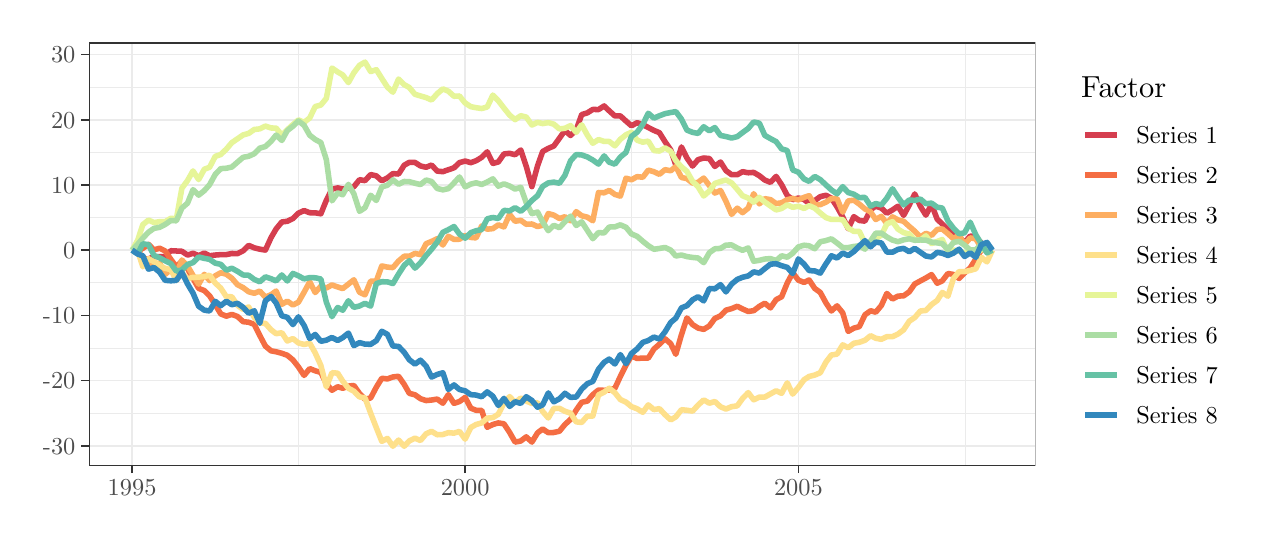
\begin{tikzpicture}[x=1pt,y=1pt]
\definecolor{fillColor}{RGB}{255,255,255}
\path[use as bounding box,fill=fillColor,fill opacity=0.00] (0,0) rectangle (441.02,176.41);
\begin{scope}
\path[clip] (  0.00,  0.00) rectangle (441.02,176.41);
\definecolor{drawColor}{RGB}{255,255,255}
\definecolor{fillColor}{RGB}{255,255,255}

\path[draw=drawColor,line width= 0.6pt,line join=round,line cap=round,fill=fillColor] (  0.00,  0.00) rectangle (441.02,176.41);
\end{scope}
\begin{scope}
\path[clip] ( 22.18, 18.22) rectangle (364.16,170.91);
\definecolor{fillColor}{RGB}{255,255,255}

\path[fill=fillColor] ( 22.18, 18.22) rectangle (364.16,170.91);
\definecolor{drawColor}{gray}{0.92}

\path[draw=drawColor,line width= 0.3pt,line join=round] ( 22.18, 37.12) --
	(364.16, 37.12);

\path[draw=drawColor,line width= 0.3pt,line join=round] ( 22.18, 60.68) --
	(364.16, 60.68);

\path[draw=drawColor,line width= 0.3pt,line join=round] ( 22.18, 84.23) --
	(364.16, 84.23);

\path[draw=drawColor,line width= 0.3pt,line join=round] ( 22.18,107.79) --
	(364.16,107.79);

\path[draw=drawColor,line width= 0.3pt,line join=round] ( 22.18,131.35) --
	(364.16,131.35);

\path[draw=drawColor,line width= 0.3pt,line join=round] ( 22.18,154.90) --
	(364.16,154.90);

\path[draw=drawColor,line width= 0.3pt,line join=round] ( 97.90, 18.22) --
	( 97.90,170.91);

\path[draw=drawColor,line width= 0.3pt,line join=round] (218.28, 18.22) --
	(218.28,170.91);

\path[draw=drawColor,line width= 0.3pt,line join=round] (338.67, 18.22) --
	(338.67,170.91);

\path[draw=drawColor,line width= 0.6pt,line join=round] ( 22.18, 25.34) --
	(364.16, 25.34);

\path[draw=drawColor,line width= 0.6pt,line join=round] ( 22.18, 48.90) --
	(364.16, 48.90);

\path[draw=drawColor,line width= 0.6pt,line join=round] ( 22.18, 72.46) --
	(364.16, 72.46);

\path[draw=drawColor,line width= 0.6pt,line join=round] ( 22.18, 96.01) --
	(364.16, 96.01);

\path[draw=drawColor,line width= 0.6pt,line join=round] ( 22.18,119.57) --
	(364.16,119.57);

\path[draw=drawColor,line width= 0.6pt,line join=round] ( 22.18,143.13) --
	(364.16,143.13);

\path[draw=drawColor,line width= 0.6pt,line join=round] ( 22.18,166.68) --
	(364.16,166.68);

\path[draw=drawColor,line width= 0.6pt,line join=round] ( 37.73, 18.22) --
	( 37.73,170.91);

\path[draw=drawColor,line width= 0.6pt,line join=round] (158.08, 18.22) --
	(158.08,170.91);

\path[draw=drawColor,line width= 0.6pt,line join=round] (278.49, 18.22) --
	(278.49,170.91);
\definecolor{drawColor}{RGB}{213,62,79}

\path[draw=drawColor,line width= 2.0pt,line join=round] ( 37.73, 96.01) --
	( 39.77, 95.28) --
	( 41.61, 92.97) --
	( 43.66, 92.85) --
	( 45.63, 93.68) --
	( 47.68, 93.71) --
	( 49.65, 93.67) --
	( 51.70, 95.81) --
	( 53.74, 95.71) --
	( 55.72, 95.61) --
	( 57.76, 94.23) --
	( 59.74, 94.89) --
	( 61.78, 94.04) --
	( 63.83, 94.97) --
	( 65.74, 94.01) --
	( 67.78, 94.25) --
	( 69.76, 94.40) --
	( 71.80, 94.42) --
	( 73.78, 94.81) --
	( 75.82, 94.76) --
	( 77.86, 95.79) --
	( 79.84, 97.75) --
	( 81.88, 96.86) --
	( 83.86, 96.37) --
	( 85.90, 96.04) --
	( 87.95,100.55) --
	( 89.79,103.71) --
	( 91.84,106.20) --
	( 93.81,106.45) --
	( 95.86,107.45) --
	( 97.83,109.38) --
	( 99.88,110.32) --
	(101.92,109.53) --
	(103.90,109.51) --
	(105.94,109.15) --
	(107.92,114.04) --
	(109.96,118.09) --
	(112.01,118.51) --
	(113.85,118.15) --
	(115.89,118.41) --
	(117.87,118.95) --
	(119.91,121.48) --
	(121.89,121.14) --
	(123.93,123.33) --
	(125.98,122.87) --
	(127.96,121.08) --
	(130.00,122.13) --
	(131.98,123.69) --
	(134.02,123.52) --
	(136.06,126.71) --
	(137.91,127.75) --
	(139.95,127.71) --
	(141.93,126.45) --
	(143.97,125.96) --
	(145.95,126.77) --
	(147.99,124.58) --
	(150.03,124.38) --
	(152.01,125.07) --
	(154.06,125.77) --
	(156.03,127.65) --
	(158.08,128.21) --
	(160.12,127.63) --
	(162.03,128.32) --
	(164.07,129.56) --
	(166.05,131.55) --
	(168.09,127.37) --
	(170.07,127.87) --
	(172.11,130.79) --
	(174.16,131.00) --
	(176.13,130.51) --
	(178.18,132.22) --
	(180.16,126.32) --
	(182.20,118.97) --
	(184.24,126.48) --
	(186.09,131.66) --
	(188.13,132.79) --
	(190.11,133.64) --
	(192.15,136.45) --
	(194.13,139.25) --
	(196.17,137.44) --
	(198.21,139.47) --
	(200.19,145.01) --
	(202.23,145.62) --
	(204.21,146.87) --
	(206.26,146.81) --
	(208.30,148.12) --
	(210.14,146.36) --
	(212.19,144.51) --
	(214.16,144.53) --
	(216.21,142.65) --
	(218.18,140.94) --
	(220.23,142.09) --
	(222.27,141.36) --
	(224.25,140.34) --
	(226.29,139.28) --
	(228.27,138.47) --
	(230.31,135.19) --
	(232.36,132.24) --
	(234.20,126.78) --
	(236.24,133.31) --
	(238.22,129.30) --
	(240.26,126.40) --
	(242.24,128.72) --
	(244.28,129.32) --
	(246.33,129.12) --
	(248.31,126.26) --
	(250.35,127.87) --
	(252.33,124.75) --
	(254.37,123.27) --
	(256.41,123.27) --
	(258.32,124.37) --
	(260.37,123.98) --
	(262.34,124.11) --
	(264.39,122.91) --
	(266.36,121.34) --
	(268.41,120.51) --
	(270.45,122.66) --
	(272.43,119.67) --
	(274.47,115.77) --
	(276.45,114.27) --
	(278.49,114.85) --
	(280.54,114.31) --
	(282.38,112.89) --
	(284.42,113.93) --
	(286.40,115.35) --
	(288.44,115.85) --
	(290.42,114.81) --
	(292.46,111.67) --
	(294.51,108.01) --
	(296.49,103.76) --
	(298.53,108.13) --
	(300.51,106.74) --
	(302.55,106.50) --
	(304.59,110.65) --
	(306.44,111.91) --
	(308.48,111.23) --
	(310.46,109.38) --
	(312.50,110.55) --
	(314.48,111.89) --
	(316.52,108.58) --
	(318.56,112.32) --
	(320.54,116.33) --
	(322.59,111.85) --
	(324.56,108.66) --
	(326.61,112.51) --
	(328.65,107.21) --
	(330.49,105.46) --
	(332.54,103.39) --
	(334.51,101.84) --
	(336.56,100.99) --
	(338.54, 98.69) --
	(340.58,101.14) --
	(342.62,100.65) --
	(344.60, 98.60) --
	(346.64, 95.51) --
	(348.62, 96.01);
\definecolor{drawColor}{RGB}{244,109,67}

\path[draw=drawColor,line width= 2.0pt,line join=round] ( 37.73, 96.01) --
	( 39.77, 95.71) --
	( 41.61, 96.67) --
	( 43.66, 98.10) --
	( 45.63, 96.11) --
	( 47.68, 96.71) --
	( 49.65, 95.75) --
	( 51.70, 92.74) --
	( 53.74, 89.99) --
	( 55.72, 92.03) --
	( 57.76, 89.33) --
	( 59.74, 85.75) --
	( 61.78, 82.21) --
	( 63.83, 81.40) --
	( 65.74, 79.53) --
	( 67.78, 76.27) --
	( 69.76, 72.98) --
	( 71.80, 72.16) --
	( 73.78, 72.80) --
	( 75.82, 72.04) --
	( 77.86, 70.17) --
	( 79.84, 69.97) --
	( 81.88, 69.19) --
	( 83.86, 65.21) --
	( 85.90, 61.34) --
	( 87.95, 59.63) --
	( 89.79, 59.30) --
	( 91.84, 58.74) --
	( 93.81, 58.03) --
	( 95.86, 56.34) --
	( 97.83, 53.83) --
	( 99.88, 50.76) --
	(101.92, 53.21) --
	(103.90, 52.42) --
	(105.94, 51.83) --
	(107.92, 47.75) --
	(109.96, 45.39) --
	(112.01, 46.66) --
	(113.85, 46.10) --
	(115.89, 46.90) --
	(117.87, 47.11) --
	(119.91, 44.22) --
	(121.89, 42.16) --
	(123.93, 42.60) --
	(125.98, 46.50) --
	(127.96, 49.72) --
	(130.00, 49.49) --
	(131.98, 50.20) --
	(134.02, 50.44) --
	(136.06, 47.51) --
	(137.91, 44.27) --
	(139.95, 43.75) --
	(141.93, 42.35) --
	(143.97, 41.66) --
	(145.95, 41.86) --
	(147.99, 42.20) --
	(150.03, 40.71) --
	(152.01, 43.81) --
	(154.06, 40.65) --
	(156.03, 41.31) --
	(158.08, 42.80) --
	(160.12, 38.92) --
	(162.03, 38.16) --
	(164.07, 38.13) --
	(166.05, 32.01) --
	(168.09, 33.02) --
	(170.07, 33.59) --
	(172.11, 33.26) --
	(174.16, 30.13) --
	(176.13, 26.66) --
	(178.18, 27.05) --
	(180.16, 28.55) --
	(182.20, 26.66) --
	(184.24, 30.00) --
	(186.09, 31.40) --
	(188.13, 30.05) --
	(190.11, 30.13) --
	(192.15, 30.59) --
	(194.13, 33.01) --
	(196.17, 34.87) --
	(198.21, 38.23) --
	(200.19, 41.04) --
	(202.23, 41.47) --
	(204.21, 43.82) --
	(206.26, 45.47) --
	(208.30, 45.37) --
	(210.14, 45.48) --
	(212.19, 46.12) --
	(214.16, 50.38) --
	(216.21, 54.47) --
	(218.18, 57.77) --
	(220.23, 56.87) --
	(222.27, 57.03) --
	(224.25, 57.00) --
	(226.29, 60.28) --
	(228.27, 62.01) --
	(230.31, 63.99) --
	(232.36, 62.23) --
	(234.20, 58.38) --
	(236.24, 65.46) --
	(238.22, 71.52) --
	(240.26, 69.12) --
	(242.24, 67.86) --
	(244.28, 67.39) --
	(246.33, 68.65) --
	(248.31, 71.34) --
	(250.35, 72.28) --
	(252.33, 74.33) --
	(254.37, 74.89) --
	(256.41, 75.74) --
	(258.32, 74.76) --
	(260.37, 73.86) --
	(262.34, 74.15) --
	(264.39, 75.70) --
	(266.36, 76.84) --
	(268.41, 75.16) --
	(270.45, 78.13) --
	(272.43, 79.17) --
	(274.47, 84.14) --
	(276.45, 87.84) --
	(278.49, 85.17) --
	(280.54, 84.35) --
	(282.38, 85.23) --
	(284.42, 82.17) --
	(286.40, 80.74) --
	(288.44, 77.00) --
	(290.42, 74.03) --
	(292.46, 75.89) --
	(294.51, 73.37) --
	(296.49, 66.67) --
	(298.53, 67.83) --
	(300.51, 68.38) --
	(302.55, 72.65) --
	(304.59, 74.12) --
	(306.44, 73.59) --
	(308.48, 76.03) --
	(310.46, 80.37) --
	(312.50, 78.34) --
	(314.48, 79.41) --
	(316.52, 79.51) --
	(318.56, 80.96) --
	(320.54, 83.79) --
	(322.59, 84.91) --
	(324.56, 85.96) --
	(326.61, 87.19) --
	(328.65, 84.07) --
	(330.49, 84.92) --
	(332.54, 87.59) --
	(334.51, 87.23) --
	(336.56, 85.79) --
	(338.54, 87.79) --
	(340.58, 89.61) --
	(342.62, 92.84) --
	(344.60, 96.05) --
	(346.64, 96.94) --
	(348.62, 96.01);
\definecolor{drawColor}{RGB}{253,174,97}

\path[draw=drawColor,line width= 2.0pt,line join=round] ( 37.73, 96.01) --
	( 39.77, 95.56) --
	( 41.61, 93.71) --
	( 43.66, 91.17) --
	( 45.63, 90.85) --
	( 47.68, 91.33) --
	( 49.65, 87.24) --
	( 51.70, 89.02) --
	( 53.74, 87.43) --
	( 55.72, 92.47) --
	( 57.76, 90.29) --
	( 59.74, 86.90) --
	( 61.78, 83.71) --
	( 63.83, 87.29) --
	( 65.74, 85.02) --
	( 67.78, 86.73) --
	( 69.76, 87.86) --
	( 71.80, 87.31) --
	( 73.78, 85.87) --
	( 75.82, 83.52) --
	( 77.86, 82.47) --
	( 79.84, 80.98) --
	( 81.88, 80.43) --
	( 83.86, 81.23) --
	( 85.90, 79.03) --
	( 87.95, 79.92) --
	( 89.79, 81.25) --
	( 91.84, 76.44) --
	( 93.81, 77.59) --
	( 95.86, 76.19) --
	( 97.83, 77.20) --
	( 99.88, 80.82) --
	(101.92, 84.56) --
	(103.90, 80.70) --
	(105.94, 82.99) --
	(107.92, 82.33) --
	(109.96, 83.45) --
	(112.01, 82.71) --
	(113.85, 82.13) --
	(115.89, 83.74) --
	(117.87, 85.32) --
	(119.91, 80.79) --
	(121.89, 79.87) --
	(123.93, 84.83) --
	(125.98, 84.85) --
	(127.96, 90.31) --
	(130.00, 89.88) --
	(131.98, 89.72) --
	(134.02, 92.08) --
	(136.06, 93.82) --
	(137.91, 93.81) --
	(139.95, 94.85) --
	(141.93, 94.40) --
	(143.97, 98.36) --
	(145.95, 99.17) --
	(147.99,100.17) --
	(150.03, 97.88) --
	(152.01,101.03) --
	(154.06, 99.89) --
	(156.03, 99.97) --
	(158.08,101.34) --
	(160.12,100.62) --
	(162.03,100.44) --
	(164.07,104.78) --
	(166.05,103.60) --
	(168.09,103.79) --
	(170.07,105.16) --
	(172.11,104.41) --
	(174.16,108.94) --
	(176.13,106.44) --
	(178.18,106.80) --
	(180.16,105.37) --
	(182.20,105.47) --
	(184.24,104.55) --
	(186.09,105.00) --
	(188.13,109.24) --
	(190.11,108.68) --
	(192.15,107.45) --
	(194.13,108.08) --
	(196.17,106.62) --
	(198.21,109.94) --
	(200.19,108.44) --
	(202.23,107.94) --
	(204.21,106.63) --
	(206.26,116.85) --
	(208.30,116.74) --
	(210.14,117.60) --
	(212.19,116.16) --
	(214.16,115.54) --
	(216.21,122.03) --
	(218.18,121.43) --
	(220.23,122.59) --
	(222.27,122.35) --
	(224.25,124.94) --
	(226.29,124.36) --
	(228.27,123.41) --
	(230.31,125.10) --
	(232.36,124.70) --
	(234.20,126.24) --
	(236.24,122.27) --
	(238.22,121.86) --
	(240.26,120.24) --
	(242.24,120.51) --
	(244.28,122.06) --
	(246.33,119.36) --
	(248.31,116.64) --
	(250.35,117.59) --
	(252.33,113.66) --
	(254.37,108.95) --
	(256.41,111.18) --
	(258.32,109.57) --
	(260.37,111.21) --
	(262.34,116.43) --
	(264.39,112.74) --
	(266.36,114.62) --
	(268.41,114.27) --
	(270.45,112.83) --
	(272.43,113.13) --
	(274.47,114.26) --
	(276.45,114.72) --
	(278.49,114.16) --
	(280.54,115.10) --
	(282.38,115.71) --
	(284.42,112.36) --
	(286.40,112.46) --
	(288.44,113.36) --
	(290.42,114.68) --
	(292.46,114.66) --
	(294.51,109.74) --
	(296.49,113.81) --
	(298.53,114.07) --
	(300.51,112.64) --
	(302.55,110.90) --
	(304.59,109.85) --
	(306.44,107.08) --
	(308.48,108.25) --
	(310.46,105.64) --
	(312.50,108.04) --
	(314.48,106.96) --
	(316.52,106.44) --
	(318.56,104.58) --
	(320.54,102.88) --
	(322.59,100.76) --
	(324.56,102.09) --
	(326.61,101.35) --
	(328.65,103.50) --
	(330.49,103.68) --
	(332.54,101.94) --
	(334.51,100.18) --
	(336.56,101.46) --
	(338.54, 98.06) --
	(340.58,100.44) --
	(342.62,100.12) --
	(344.60, 96.76) --
	(346.64, 95.43) --
	(348.62, 96.01);
\definecolor{drawColor}{RGB}{254,224,139}

\path[draw=drawColor,line width= 2.0pt,line join=round] ( 37.73, 96.01) --
	( 39.77, 95.78) --
	( 41.61, 90.01) --
	( 43.66, 92.93) --
	( 45.63, 91.88) --
	( 47.68, 90.54) --
	( 49.65, 89.43) --
	( 51.70, 89.01) --
	( 53.74, 85.07) --
	( 55.72, 87.76) --
	( 57.76, 85.70) --
	( 59.74, 86.18) --
	( 61.78, 86.26) --
	( 63.83, 86.47) --
	( 65.74, 86.95) --
	( 67.78, 84.14) --
	( 69.76, 82.31) --
	( 71.80, 79.18) --
	( 73.78, 79.17) --
	( 75.82, 76.07) --
	( 77.86, 74.60) --
	( 79.84, 75.49) --
	( 81.88, 71.71) --
	( 83.86, 69.71) --
	( 85.90, 69.54) --
	( 87.95, 67.24) --
	( 89.79, 65.83) --
	( 91.84, 66.18) --
	( 93.81, 63.20) --
	( 95.86, 64.07) --
	( 97.83, 62.49) --
	( 99.88, 61.94) --
	(101.92, 62.39) --
	(103.90, 58.89) --
	(105.94, 54.36) --
	(107.92, 46.60) --
	(109.96, 51.73) --
	(112.01, 51.57) --
	(113.85, 48.68) --
	(115.89, 46.10) --
	(117.87, 45.05) --
	(119.91, 42.98) --
	(121.89, 42.66) --
	(123.93, 37.12) --
	(125.98, 31.86) --
	(127.96, 26.95) --
	(130.00, 27.98) --
	(131.98, 25.16) --
	(134.02, 27.39) --
	(136.06, 25.16) --
	(137.91, 27.10) --
	(139.95, 28.07) --
	(141.93, 27.22) --
	(143.97, 29.67) --
	(145.95, 30.54) --
	(147.99, 29.31) --
	(150.03, 29.40) --
	(152.01, 30.07) --
	(154.06, 29.89) --
	(156.03, 30.54) --
	(158.08, 27.72) --
	(160.12, 31.93) --
	(162.03, 33.01) --
	(164.07, 33.59) --
	(166.05, 35.31) --
	(168.09, 35.51) --
	(170.07, 36.72) --
	(172.11, 40.76) --
	(174.16, 43.10) --
	(176.13, 40.94) --
	(178.18, 42.59) --
	(180.16, 41.49) --
	(182.20, 40.63) --
	(184.24, 40.93) --
	(186.09, 37.72) --
	(188.13, 35.37) --
	(190.11, 38.83) --
	(192.15, 38.86) --
	(194.13, 37.79) --
	(196.17, 37.13) --
	(198.21, 33.96) --
	(200.19, 33.76) --
	(202.23, 36.06) --
	(204.21, 36.08) --
	(206.26, 43.70) --
	(208.30, 44.72) --
	(210.14, 46.13) --
	(212.19, 44.50) --
	(214.16, 42.03) --
	(216.21, 41.09) --
	(218.18, 39.47) --
	(220.23, 38.69) --
	(222.27, 37.43) --
	(224.25, 40.10) --
	(226.29, 38.39) --
	(228.27, 38.75) --
	(230.31, 36.56) --
	(232.36, 34.68) --
	(234.20, 35.77) --
	(236.24, 38.36) --
	(238.22, 38.16) --
	(240.26, 37.86) --
	(242.24, 40.01) --
	(244.28, 41.90) --
	(246.33, 40.72) --
	(248.31, 41.32) --
	(250.35, 39.41) --
	(252.33, 38.61) --
	(254.37, 39.46) --
	(256.41, 39.75) --
	(258.32, 42.41) --
	(260.37, 44.53) --
	(262.34, 41.94) --
	(264.39, 42.91) --
	(266.36, 42.92) --
	(268.41, 44.08) --
	(270.45, 45.20) --
	(272.43, 44.28) --
	(274.47, 48.06) --
	(276.45, 44.01) --
	(278.49, 46.40) --
	(280.54, 49.20) --
	(282.38, 50.37) --
	(284.42, 50.89) --
	(286.40, 51.71) --
	(288.44, 55.53) --
	(290.42, 58.14) --
	(292.46, 58.45) --
	(294.51, 61.81) --
	(296.49, 60.74) --
	(298.53, 62.38) --
	(300.51, 62.72) --
	(302.55, 63.45) --
	(304.59, 65.11) --
	(306.44, 64.18) --
	(308.48, 63.80) --
	(310.46, 64.75) --
	(312.50, 64.76) --
	(314.48, 65.70) --
	(316.52, 67.23) --
	(318.56, 70.34) --
	(320.54, 71.66) --
	(322.59, 74.04) --
	(324.56, 74.23) --
	(326.61, 76.36) --
	(328.65, 77.83) --
	(330.49, 80.74) --
	(332.54, 79.37) --
	(334.51, 85.79) --
	(336.56, 88.25) --
	(338.54, 88.26) --
	(340.58, 88.70) --
	(342.62, 89.28) --
	(344.60, 93.43) --
	(346.64, 91.79) --
	(348.62, 96.01);
\definecolor{drawColor}{RGB}{230,245,152}

\path[draw=drawColor,line width= 2.0pt,line join=round] ( 37.73, 96.01) --
	( 39.77, 99.64) --
	( 41.61,105.25) --
	( 43.66,106.88) --
	( 45.63,105.99) --
	( 47.68,106.31) --
	( 49.65,106.29) --
	( 51.70,107.52) --
	( 53.74,107.36) --
	( 55.72,118.37) --
	( 57.76,121.16) --
	( 59.74,124.64) --
	( 61.78,121.51) --
	( 63.83,125.25) --
	( 65.74,125.97) --
	( 67.78,129.90) --
	( 69.76,130.57) --
	( 71.80,132.54) --
	( 73.78,134.86) --
	( 75.82,136.26) --
	( 77.86,137.66) --
	( 79.84,138.20) --
	( 81.88,139.62) --
	( 83.86,139.84) --
	( 85.90,140.86) --
	( 87.95,140.16) --
	( 89.79,140.13) --
	( 91.84,137.54) --
	( 93.81,139.53) --
	( 95.86,141.42) --
	( 97.83,143.07) --
	( 99.88,142.20) --
	(101.92,143.77) --
	(103.90,147.91) --
	(105.94,148.45) --
	(107.92,150.86) --
	(109.96,161.82) --
	(112.01,160.40) --
	(113.85,159.35) --
	(115.89,156.56) --
	(117.87,160.13) --
	(119.91,162.80) --
	(121.89,163.97) --
	(123.93,160.54) --
	(125.98,161.24) --
	(127.96,158.07) --
	(130.00,154.91) --
	(131.98,153.09) --
	(134.02,157.86) --
	(136.06,155.82) --
	(137.91,154.78) --
	(139.95,152.33) --
	(141.93,151.74) --
	(143.97,151.14) --
	(145.95,150.27) --
	(147.99,152.57) --
	(150.03,154.29) --
	(152.01,153.44) --
	(154.06,151.62) --
	(156.03,151.72) --
	(158.08,149.18) --
	(160.12,147.86) --
	(162.03,147.49) --
	(164.07,147.19) --
	(166.05,147.74) --
	(168.09,152.05) --
	(170.07,150.00) --
	(172.11,147.36) --
	(174.16,144.81) --
	(176.13,143.18) --
	(178.18,144.61) --
	(180.16,144.10) --
	(182.20,141.22) --
	(184.24,142.21) --
	(186.09,141.76) --
	(188.13,142.10) --
	(190.11,141.55) --
	(192.15,139.81) --
	(194.13,140.05) --
	(196.17,141.03) --
	(198.21,138.56) --
	(200.19,141.31) --
	(202.23,137.60) --
	(204.21,134.65) --
	(206.26,135.97) --
	(208.30,135.32) --
	(210.14,135.28) --
	(212.19,133.72) --
	(214.16,136.08) --
	(216.21,137.72) --
	(218.18,138.63) --
	(220.23,135.73) --
	(222.27,135.03) --
	(224.25,135.41) --
	(226.29,132.00) --
	(228.27,131.83) --
	(230.31,132.98) --
	(232.36,131.75) --
	(234.20,128.38) --
	(236.24,126.12) --
	(238.22,124.47) --
	(240.26,120.90) --
	(242.24,118.95) --
	(244.28,115.58) --
	(246.33,117.40) --
	(248.31,120.12) --
	(250.35,120.82) --
	(252.33,121.38) --
	(254.37,120.31) --
	(256.41,117.98) --
	(258.32,115.66) --
	(260.37,114.83) --
	(262.34,113.37) --
	(264.39,115.09) --
	(266.36,113.42) --
	(268.41,111.97) --
	(270.45,110.55) --
	(272.43,111.07) --
	(274.47,112.40) --
	(276.45,111.50) --
	(278.49,111.89) --
	(280.54,111.08) --
	(282.38,112.08) --
	(284.42,111.18) --
	(286.40,109.45) --
	(288.44,107.78) --
	(290.42,107.13) --
	(292.46,107.14) --
	(294.51,107.06) --
	(296.49,104.02) --
	(298.53,102.79) --
	(300.51,102.83) --
	(302.55, 98.50) --
	(304.59, 98.76) --
	(306.44,100.20) --
	(308.48,101.43) --
	(310.46,105.53) --
	(312.50,106.33) --
	(314.48,103.61) --
	(316.52,102.34) --
	(318.56,101.86) --
	(320.54, 99.73) --
	(322.59, 99.66) --
	(324.56,101.19) --
	(326.61, 98.40) --
	(328.65, 99.15) --
	(330.49, 99.85) --
	(332.54, 95.27) --
	(334.51, 96.07) --
	(336.56, 95.69) --
	(338.54, 95.06) --
	(340.58, 94.85) --
	(342.62, 94.66) --
	(344.60, 96.21) --
	(346.64, 96.29) --
	(348.62, 96.01);
\definecolor{drawColor}{RGB}{171,221,164}

\path[draw=drawColor,line width= 2.0pt,line join=round] ( 37.73, 96.01) --
	( 39.77, 98.14) --
	( 41.61,100.36) --
	( 43.66,102.50) --
	( 45.63,103.89) --
	( 47.68,104.26) --
	( 49.65,105.27) --
	( 51.70,106.71) --
	( 53.74,106.63) --
	( 55.72,111.23) --
	( 57.76,112.99) --
	( 59.74,117.88) --
	( 61.78,115.89) --
	( 63.83,117.53) --
	( 65.74,119.67) --
	( 67.78,123.39) --
	( 69.76,125.47) --
	( 71.80,125.62) --
	( 73.78,126.05) --
	( 75.82,127.83) --
	( 77.86,129.57) --
	( 79.84,129.93) --
	( 81.88,130.87) --
	( 83.86,132.87) --
	( 85.90,133.46) --
	( 87.95,135.35) --
	( 89.79,137.61) --
	( 91.84,135.65) --
	( 93.81,139.22) --
	( 95.86,140.80) --
	( 97.83,142.69) --
	( 99.88,141.12) --
	(101.92,137.55) --
	(103.90,136.01) --
	(105.94,134.90) --
	(107.92,128.75) --
	(109.96,113.82) --
	(112.01,116.70) --
	(113.85,116.03) --
	(115.89,119.80) --
	(117.87,116.38) --
	(119.91,110.05) --
	(121.89,111.35) --
	(123.93,115.86) --
	(125.98,113.96) --
	(127.96,118.87) --
	(130.00,119.47) --
	(131.98,121.44) --
	(134.02,119.81) --
	(136.06,120.83) --
	(137.91,120.75) --
	(139.95,120.20) --
	(141.93,119.72) --
	(143.97,121.35) --
	(145.95,120.83) --
	(147.99,118.30) --
	(150.03,117.81) --
	(152.01,118.24) --
	(154.06,120.32) --
	(156.03,122.46) --
	(158.08,118.89) --
	(160.12,119.87) --
	(162.03,120.36) --
	(164.07,119.75) --
	(166.05,120.64) --
	(168.09,121.79) --
	(170.07,119.14) --
	(172.11,119.97) --
	(174.16,119.19) --
	(176.13,118.08) --
	(178.18,118.72) --
	(180.16,113.14) --
	(182.20,109.21) --
	(184.24,109.79) --
	(186.09,106.19) --
	(188.13,103.05) --
	(190.11,104.99) --
	(192.15,104.12) --
	(194.13,106.28) --
	(196.17,108.31) --
	(198.21,104.92) --
	(200.19,106.24) --
	(202.23,103.16) --
	(204.21,100.15) --
	(206.26,102.38) --
	(208.30,102.23) --
	(210.14,104.37) --
	(212.19,104.44) --
	(214.16,105.17) --
	(216.21,104.27) --
	(218.18,101.88) --
	(220.23,101.00) --
	(222.27, 99.23) --
	(224.25, 97.65) --
	(226.29, 96.33) --
	(228.27, 96.63) --
	(230.31, 96.98) --
	(232.36, 96.03) --
	(234.20, 93.89) --
	(236.24, 94.26) --
	(238.22, 93.69) --
	(240.26, 93.38) --
	(242.24, 93.18) --
	(244.28, 91.50) --
	(246.33, 95.10) --
	(248.31, 96.51) --
	(250.35, 96.65) --
	(252.33, 97.85) --
	(254.37, 97.90) --
	(256.41, 96.77) --
	(258.32, 95.95) --
	(260.37, 96.81) --
	(262.34, 92.01) --
	(264.39, 92.34) --
	(266.36, 92.81) --
	(268.41, 92.97) --
	(270.45, 92.26) --
	(272.43, 93.98) --
	(274.47, 93.47) --
	(276.45, 94.91) --
	(278.49, 97.18) --
	(280.54, 97.80) --
	(282.38, 97.58) --
	(284.42, 96.54) --
	(286.40, 99.04) --
	(288.44, 99.47) --
	(290.42,100.11) --
	(292.46, 98.60) --
	(294.51, 96.96) --
	(296.49, 96.93) --
	(298.53, 97.34) --
	(300.51, 97.61) --
	(302.55, 96.38) --
	(304.59, 99.35) --
	(306.44,102.16) --
	(308.48,102.19) --
	(310.46,100.78) --
	(312.50, 99.64) --
	(314.48, 99.08) --
	(316.52, 99.75) --
	(318.56,100.13) --
	(320.54, 99.58) --
	(322.59, 99.70) --
	(324.56, 99.63) --
	(326.61, 98.94) --
	(328.65, 98.64) --
	(330.49, 98.36) --
	(332.54, 96.29) --
	(334.51, 98.78) --
	(336.56, 99.21) --
	(338.54, 97.81) --
	(340.58, 96.08) --
	(342.62, 96.14) --
	(344.60, 98.31) --
	(346.64, 96.93) --
	(348.62, 96.01);
\definecolor{drawColor}{RGB}{102,194,165}

\path[draw=drawColor,line width= 2.0pt,line join=round] ( 37.73, 96.01) --
	( 39.77, 94.71) --
	( 41.61, 98.31) --
	( 43.66, 97.99) --
	( 45.63, 94.12) --
	( 47.68, 93.25) --
	( 49.65, 92.17) --
	( 51.70, 91.19) --
	( 53.74, 88.43) --
	( 55.72, 88.87) --
	( 57.76, 90.85) --
	( 59.74, 91.50) --
	( 61.78, 93.56) --
	( 63.83, 93.05) --
	( 65.74, 92.70) --
	( 67.78, 91.32) --
	( 69.76, 90.89) --
	( 71.80, 88.79) --
	( 73.78, 89.49) --
	( 75.82, 88.36) --
	( 77.86, 87.05) --
	( 79.84, 86.94) --
	( 81.88, 85.44) --
	( 83.86, 84.59) --
	( 85.90, 86.36) --
	( 87.95, 85.69) --
	( 89.79, 84.91) --
	( 91.84, 87.05) --
	( 93.81, 84.88) --
	( 95.86, 87.61) --
	( 97.83, 86.74) --
	( 99.88, 85.63) --
	(101.92, 86.10) --
	(103.90, 86.03) --
	(105.94, 85.60) --
	(107.92, 77.21) --
	(109.96, 71.99) --
	(112.01, 75.30) --
	(113.85, 74.30) --
	(115.89, 77.73) --
	(117.87, 75.35) --
	(119.91, 75.84) --
	(121.89, 76.81) --
	(123.93, 75.80) --
	(125.98, 83.93) --
	(127.96, 84.61) --
	(130.00, 84.56) --
	(131.98, 83.95) --
	(134.02, 87.38) --
	(136.06, 90.53) --
	(137.91, 92.20) --
	(139.95, 89.53) --
	(141.93, 91.43) --
	(143.97, 94.07) --
	(145.95, 96.34) --
	(147.99, 98.93) --
	(150.03,102.46) --
	(152.01,103.41) --
	(154.06,104.55) --
	(156.03,101.83) --
	(158.08,100.34) --
	(160.12,102.33) --
	(162.03,103.03) --
	(164.07,103.46) --
	(166.05,107.33) --
	(168.09,107.83) --
	(170.07,107.44) --
	(172.11,110.40) --
	(174.16,110.19) --
	(176.13,111.38) --
	(178.18,110.05) --
	(180.16,111.75) --
	(182.20,113.97) --
	(184.24,115.69) --
	(186.09,119.05) --
	(188.13,120.32) --
	(190.11,120.60) --
	(192.15,120.19) --
	(194.13,123.04) --
	(196.17,128.32) --
	(198.21,130.57) --
	(200.19,130.42) --
	(202.23,129.70) --
	(204.21,128.58) --
	(206.26,127.12) --
	(208.30,130.07) --
	(210.14,127.79) --
	(212.19,127.09) --
	(214.16,129.65) --
	(216.21,131.34) --
	(218.18,137.14) --
	(220.23,138.65) --
	(222.27,141.44) --
	(224.25,145.48) --
	(226.29,143.72) --
	(228.27,144.57) --
	(230.31,145.34) --
	(232.36,145.75) --
	(234.20,146.09) --
	(236.24,143.36) --
	(238.22,139.40) --
	(240.26,138.58) --
	(242.24,138.20) --
	(244.28,140.62) --
	(246.33,139.12) --
	(248.31,140.33) --
	(250.35,137.46) --
	(252.33,137.07) --
	(254.37,136.53) --
	(256.41,137.05) --
	(258.32,138.50) --
	(260.37,139.99) --
	(262.34,142.33) --
	(264.39,141.90) --
	(266.36,137.48) --
	(268.41,136.32) --
	(270.45,135.23) --
	(272.43,132.61) --
	(274.47,132.02) --
	(276.45,124.99) --
	(278.49,124.19) --
	(280.54,121.72) --
	(282.38,120.88) --
	(284.42,122.65) --
	(286.40,121.51) --
	(288.44,119.60) --
	(290.42,117.78) --
	(292.46,116.36) --
	(294.51,118.98) --
	(296.49,116.84) --
	(298.53,116.23) --
	(300.51,115.01) --
	(302.55,115.07) --
	(304.59,111.93) --
	(306.44,112.84) --
	(308.48,112.35) --
	(310.46,114.81) --
	(312.50,118.19) --
	(314.48,115.14) --
	(316.52,112.36) --
	(318.56,114.16) --
	(320.54,113.98) --
	(322.59,114.48) --
	(324.56,112.80) --
	(326.61,113.01) --
	(328.65,111.54) --
	(330.49,111.24) --
	(332.54,106.54) --
	(334.51,103.99) --
	(336.56,101.93) --
	(338.54,102.27) --
	(340.58,106.12) --
	(342.62,101.53) --
	(344.60, 98.33) --
	(346.64, 95.03) --
	(348.62, 96.01);
\definecolor{drawColor}{RGB}{50,136,189}

\path[draw=drawColor,line width= 2.0pt,line join=round] ( 37.73, 96.01) --
	( 39.77, 94.60) --
	( 41.61, 93.98) --
	( 43.66, 89.15) --
	( 45.63, 89.75) --
	( 47.68, 88.05) --
	( 49.65, 85.11) --
	( 51.70, 84.94) --
	( 53.74, 85.10) --
	( 55.72, 88.04) --
	( 57.76, 83.82) --
	( 59.74, 80.51) --
	( 61.78, 75.75) --
	( 63.83, 74.33) --
	( 65.74, 74.04) --
	( 67.78, 77.54) --
	( 69.76, 75.95) --
	( 71.80, 77.55) --
	( 73.78, 76.29) --
	( 75.82, 76.81) --
	( 77.86, 75.35) --
	( 79.84, 73.22) --
	( 81.88, 74.10) --
	( 83.86, 69.59) --
	( 85.90, 77.71) --
	( 87.95, 79.31) --
	( 89.79, 76.89) --
	( 91.84, 72.29) --
	( 93.81, 71.74) --
	( 95.86, 69.11) --
	( 97.83, 71.93) --
	( 99.88, 68.83) --
	(101.92, 64.05) --
	(103.90, 65.55) --
	(105.94, 63.08) --
	(107.92, 63.49) --
	(109.96, 64.46) --
	(112.01, 63.37) --
	(113.85, 64.41) --
	(115.89, 66.05) --
	(117.87, 61.51) --
	(119.91, 62.61) --
	(121.89, 62.06) --
	(123.93, 61.99) --
	(125.98, 63.29) --
	(127.96, 66.71) --
	(130.00, 65.59) --
	(131.98, 61.36) --
	(134.02, 61.24) --
	(136.06, 59.09) --
	(137.91, 56.40) --
	(139.95, 54.84) --
	(141.93, 56.25) --
	(143.97, 54.12) --
	(145.95, 50.15) --
	(147.99, 51.11) --
	(150.03, 51.71) --
	(152.01, 45.69) --
	(154.06, 47.32) --
	(156.03, 45.66) --
	(158.08, 45.18) --
	(160.12, 43.80) --
	(162.03, 43.65) --
	(164.07, 43.05) --
	(166.05, 44.81) --
	(168.09, 43.24) --
	(170.07, 39.89) --
	(172.11, 42.45) --
	(174.16, 39.56) --
	(176.13, 41.24) --
	(178.18, 40.64) --
	(180.16, 43.06) --
	(182.20, 41.69) --
	(184.24, 39.27) --
	(186.09, 40.12) --
	(188.13, 44.43) --
	(190.11, 41.21) --
	(192.15, 42.30) --
	(194.13, 44.31) --
	(196.17, 42.82) --
	(198.21, 42.94) --
	(200.19, 45.81) --
	(202.23, 47.77) --
	(204.21, 48.59) --
	(206.26, 52.98) --
	(208.30, 55.47) --
	(210.14, 56.66) --
	(212.19, 54.88) --
	(214.16, 58.28) --
	(216.21, 55.00) --
	(218.18, 58.68) --
	(220.23, 60.34) --
	(222.27, 62.68) --
	(224.25, 63.37) --
	(226.29, 64.62) --
	(228.27, 63.89) --
	(230.31, 66.50) --
	(232.36, 69.89) --
	(234.20, 71.43) --
	(236.24, 75.16) --
	(238.22, 75.94) --
	(240.26, 78.08) --
	(242.24, 79.18) --
	(244.28, 77.68) --
	(246.33, 82.16) --
	(248.31, 82.05) --
	(250.35, 83.56) --
	(252.33, 80.94) --
	(254.37, 83.76) --
	(256.41, 85.45) --
	(258.32, 86.22) --
	(260.37, 86.70) --
	(262.34, 88.17) --
	(264.39, 87.73) --
	(266.36, 89.34) --
	(268.41, 90.95) --
	(270.45, 91.12) --
	(272.43, 90.39) --
	(274.47, 89.80) --
	(276.45, 87.55) --
	(278.49, 92.86) --
	(280.54, 90.98) --
	(282.38, 88.63) --
	(284.42, 88.51) --
	(286.40, 87.71) --
	(288.44, 91.06) --
	(290.42, 93.99) --
	(292.46, 93.18) --
	(294.51, 94.97) --
	(296.49, 94.07) --
	(298.53, 95.50) --
	(300.51, 97.51) --
	(302.55, 99.46) --
	(304.59, 97.23) --
	(306.44, 98.93) --
	(308.48, 98.61) --
	(310.46, 95.35) --
	(312.50, 95.27) --
	(314.48, 96.31) --
	(316.52, 96.65) --
	(318.56, 95.44) --
	(320.54, 96.67) --
	(322.59, 95.25) --
	(324.56, 93.89) --
	(326.61, 93.55) --
	(328.65, 95.22) --
	(330.49, 94.90) --
	(332.54, 94.10) --
	(334.51, 94.94) --
	(336.56, 96.37) --
	(338.54, 93.73) --
	(340.58, 95.03) --
	(342.62, 93.42) --
	(344.60, 98.00) --
	(346.64, 98.82) --
	(348.62, 96.01);
\definecolor{drawColor}{gray}{0.20}

\path[draw=drawColor,line width= 0.6pt,line join=round,line cap=round] ( 22.18, 18.22) rectangle (364.16,170.91);
\end{scope}
\begin{scope}
\path[clip] (  0.00,  0.00) rectangle (441.02,176.41);
\definecolor{drawColor}{gray}{0.30}

\node[text=drawColor,anchor=base east,inner sep=0pt, outer sep=0pt, scale=  0.88] at ( 17.23, 22.31) {-30};

\node[text=drawColor,anchor=base east,inner sep=0pt, outer sep=0pt, scale=  0.88] at ( 17.23, 45.87) {-20};

\node[text=drawColor,anchor=base east,inner sep=0pt, outer sep=0pt, scale=  0.88] at ( 17.23, 69.43) {-10};

\node[text=drawColor,anchor=base east,inner sep=0pt, outer sep=0pt, scale=  0.88] at ( 17.23, 92.98) {0};

\node[text=drawColor,anchor=base east,inner sep=0pt, outer sep=0pt, scale=  0.88] at ( 17.23,116.54) {10};

\node[text=drawColor,anchor=base east,inner sep=0pt, outer sep=0pt, scale=  0.88] at ( 17.23,140.10) {20};

\node[text=drawColor,anchor=base east,inner sep=0pt, outer sep=0pt, scale=  0.88] at ( 17.23,163.65) {30};
\end{scope}
\begin{scope}
\path[clip] (  0.00,  0.00) rectangle (441.02,176.41);
\definecolor{drawColor}{gray}{0.20}

\path[draw=drawColor,line width= 0.6pt,line join=round] ( 19.43, 25.34) --
	( 22.18, 25.34);

\path[draw=drawColor,line width= 0.6pt,line join=round] ( 19.43, 48.90) --
	( 22.18, 48.90);

\path[draw=drawColor,line width= 0.6pt,line join=round] ( 19.43, 72.46) --
	( 22.18, 72.46);

\path[draw=drawColor,line width= 0.6pt,line join=round] ( 19.43, 96.01) --
	( 22.18, 96.01);

\path[draw=drawColor,line width= 0.6pt,line join=round] ( 19.43,119.57) --
	( 22.18,119.57);

\path[draw=drawColor,line width= 0.6pt,line join=round] ( 19.43,143.13) --
	( 22.18,143.13);

\path[draw=drawColor,line width= 0.6pt,line join=round] ( 19.43,166.68) --
	( 22.18,166.68);
\end{scope}
\begin{scope}
\path[clip] (  0.00,  0.00) rectangle (441.02,176.41);
\definecolor{drawColor}{gray}{0.20}

\path[draw=drawColor,line width= 0.6pt,line join=round] ( 37.73, 15.47) --
	( 37.73, 18.22);

\path[draw=drawColor,line width= 0.6pt,line join=round] (158.08, 15.47) --
	(158.08, 18.22);

\path[draw=drawColor,line width= 0.6pt,line join=round] (278.49, 15.47) --
	(278.49, 18.22);
\end{scope}
\begin{scope}
\path[clip] (  0.00,  0.00) rectangle (441.02,176.41);
\definecolor{drawColor}{gray}{0.30}

\node[text=drawColor,anchor=base,inner sep=0pt, outer sep=0pt, scale=  0.88] at ( 37.73,  7.21) {1995};

\node[text=drawColor,anchor=base,inner sep=0pt, outer sep=0pt, scale=  0.88] at (158.08,  7.21) {2000};

\node[text=drawColor,anchor=base,inner sep=0pt, outer sep=0pt, scale=  0.88] at (278.49,  7.21) {2005};
\end{scope}
\begin{scope}
\path[clip] (  0.00,  0.00) rectangle (441.02,176.41);
\definecolor{fillColor}{RGB}{255,255,255}

\path[fill=fillColor] (375.16, 23.64) rectangle (435.52,165.49);
\end{scope}
\begin{scope}
\path[clip] (  0.00,  0.00) rectangle (441.02,176.41);
\definecolor{drawColor}{RGB}{0,0,0}

\node[text=drawColor,anchor=base west,inner sep=0pt, outer sep=0pt, scale=  1.10] at (380.66,151.34) {Factor};
\end{scope}
\begin{scope}
\path[clip] (  0.00,  0.00) rectangle (441.02,176.41);
\definecolor{fillColor}{RGB}{255,255,255}

\path[fill=fillColor] (380.66,130.32) rectangle (395.12,144.77);
\end{scope}
\begin{scope}
\path[clip] (  0.00,  0.00) rectangle (441.02,176.41);
\definecolor{drawColor}{RGB}{213,62,79}

\path[draw=drawColor,line width= 2.0pt,line join=round] (382.11,137.55) -- (393.67,137.55);
\end{scope}
\begin{scope}
\path[clip] (  0.00,  0.00) rectangle (441.02,176.41);
\definecolor{fillColor}{RGB}{255,255,255}

\path[fill=fillColor] (380.66,115.87) rectangle (395.12,130.32);
\end{scope}
\begin{scope}
\path[clip] (  0.00,  0.00) rectangle (441.02,176.41);
\definecolor{drawColor}{RGB}{244,109,67}

\path[draw=drawColor,line width= 2.0pt,line join=round] (382.11,123.09) -- (393.67,123.09);
\end{scope}
\begin{scope}
\path[clip] (  0.00,  0.00) rectangle (441.02,176.41);
\definecolor{fillColor}{RGB}{255,255,255}

\path[fill=fillColor] (380.66,101.41) rectangle (395.12,115.87);
\end{scope}
\begin{scope}
\path[clip] (  0.00,  0.00) rectangle (441.02,176.41);
\definecolor{drawColor}{RGB}{253,174,97}

\path[draw=drawColor,line width= 2.0pt,line join=round] (382.11,108.64) -- (393.67,108.64);
\end{scope}
\begin{scope}
\path[clip] (  0.00,  0.00) rectangle (441.02,176.41);
\definecolor{fillColor}{RGB}{255,255,255}

\path[fill=fillColor] (380.66, 86.96) rectangle (395.12,101.41);
\end{scope}
\begin{scope}
\path[clip] (  0.00,  0.00) rectangle (441.02,176.41);
\definecolor{drawColor}{RGB}{254,224,139}

\path[draw=drawColor,line width= 2.0pt,line join=round] (382.11, 94.18) -- (393.67, 94.18);
\end{scope}
\begin{scope}
\path[clip] (  0.00,  0.00) rectangle (441.02,176.41);
\definecolor{fillColor}{RGB}{255,255,255}

\path[fill=fillColor] (380.66, 72.50) rectangle (395.12, 86.96);
\end{scope}
\begin{scope}
\path[clip] (  0.00,  0.00) rectangle (441.02,176.41);
\definecolor{drawColor}{RGB}{230,245,152}

\path[draw=drawColor,line width= 2.0pt,line join=round] (382.11, 79.73) -- (393.67, 79.73);
\end{scope}
\begin{scope}
\path[clip] (  0.00,  0.00) rectangle (441.02,176.41);
\definecolor{fillColor}{RGB}{255,255,255}

\path[fill=fillColor] (380.66, 58.05) rectangle (395.12, 72.50);
\end{scope}
\begin{scope}
\path[clip] (  0.00,  0.00) rectangle (441.02,176.41);
\definecolor{drawColor}{RGB}{171,221,164}

\path[draw=drawColor,line width= 2.0pt,line join=round] (382.11, 65.28) -- (393.67, 65.28);
\end{scope}
\begin{scope}
\path[clip] (  0.00,  0.00) rectangle (441.02,176.41);
\definecolor{fillColor}{RGB}{255,255,255}

\path[fill=fillColor] (380.66, 43.60) rectangle (395.12, 58.05);
\end{scope}
\begin{scope}
\path[clip] (  0.00,  0.00) rectangle (441.02,176.41);
\definecolor{drawColor}{RGB}{102,194,165}

\path[draw=drawColor,line width= 2.0pt,line join=round] (382.11, 50.82) -- (393.67, 50.82);
\end{scope}
\begin{scope}
\path[clip] (  0.00,  0.00) rectangle (441.02,176.41);
\definecolor{fillColor}{RGB}{255,255,255}

\path[fill=fillColor] (380.66, 29.14) rectangle (395.12, 43.60);
\end{scope}
\begin{scope}
\path[clip] (  0.00,  0.00) rectangle (441.02,176.41);
\definecolor{drawColor}{RGB}{50,136,189}

\path[draw=drawColor,line width= 2.0pt,line join=round] (382.11, 36.37) -- (393.67, 36.37);
\end{scope}
\begin{scope}
\path[clip] (  0.00,  0.00) rectangle (441.02,176.41);
\definecolor{drawColor}{RGB}{0,0,0}

\node[text=drawColor,anchor=base west,inner sep=0pt, outer sep=0pt, scale=  0.88] at (400.62,134.52) {Series 1};
\end{scope}
\begin{scope}
\path[clip] (  0.00,  0.00) rectangle (441.02,176.41);
\definecolor{drawColor}{RGB}{0,0,0}

\node[text=drawColor,anchor=base west,inner sep=0pt, outer sep=0pt, scale=  0.88] at (400.62,120.06) {Series 2};
\end{scope}
\begin{scope}
\path[clip] (  0.00,  0.00) rectangle (441.02,176.41);
\definecolor{drawColor}{RGB}{0,0,0}

\node[text=drawColor,anchor=base west,inner sep=0pt, outer sep=0pt, scale=  0.88] at (400.62,105.61) {Series 3};
\end{scope}
\begin{scope}
\path[clip] (  0.00,  0.00) rectangle (441.02,176.41);
\definecolor{drawColor}{RGB}{0,0,0}

\node[text=drawColor,anchor=base west,inner sep=0pt, outer sep=0pt, scale=  0.88] at (400.62, 91.15) {Series 4};
\end{scope}
\begin{scope}
\path[clip] (  0.00,  0.00) rectangle (441.02,176.41);
\definecolor{drawColor}{RGB}{0,0,0}

\node[text=drawColor,anchor=base west,inner sep=0pt, outer sep=0pt, scale=  0.88] at (400.62, 76.70) {Series 5};
\end{scope}
\begin{scope}
\path[clip] (  0.00,  0.00) rectangle (441.02,176.41);
\definecolor{drawColor}{RGB}{0,0,0}

\node[text=drawColor,anchor=base west,inner sep=0pt, outer sep=0pt, scale=  0.88] at (400.62, 62.25) {Series 6};
\end{scope}
\begin{scope}
\path[clip] (  0.00,  0.00) rectangle (441.02,176.41);
\definecolor{drawColor}{RGB}{0,0,0}

\node[text=drawColor,anchor=base west,inner sep=0pt, outer sep=0pt, scale=  0.88] at (400.62, 47.79) {Series 7};
\end{scope}
\begin{scope}
\path[clip] (  0.00,  0.00) rectangle (441.02,176.41);
\definecolor{drawColor}{RGB}{0,0,0}

\node[text=drawColor,anchor=base west,inner sep=0pt, outer sep=0pt, scale=  0.88] at (400.62, 33.34) {Series 8};
\end{scope}
\end{tikzpicture}
}
	\label{fig:Factors}
\end{figure}
Figure~\ref{fig:Factors} depicts the \code{autoplot()} result for the common factors, which are ordered according to their decreasing eigenvalue of the PCA. Using \code{palette="Spectral"} for factors' color assignment, the transition from ``warm'' to ``cold'' colors reflects decreasing power of  the factors to explain the common variation within the observed time series. In comparison to the figure from the original study, the factors $ \boldsymbol{\hat{F}}_t $ may have switched signs and be multiplied by a scalar such that only their dynamics are informative. However, the PANIC analysis on both components is invariant to this differing normalization of loadings and factors $ \hat{\Lambda}_i' \boldsymbol{\hat{F}}_t $: \textit{(1)}~The idiosyncratic components are calculated via this complete term of common components, which the normalization does not alter. \textit{(2)}~The common factors $ \boldsymbol{\hat{F}}_{t} $ exhibit the same strength of cointegration, i.e. $ \boldsymbol{\hat{\lambda}} $ of the reduced-rank regression \eqref{eq:RRReigen}, irrespective of any scaling weight multiplied to a time series of $ \boldsymbol{\hat{F}}_{t} $.

In order to determine the cointegration rank within $ \boldsymbol{F}_{t} $, we employ the single VECM~\eqref{eq:VECM} with a linear trend in the cointegration space. The proceeding is the same as any individual analysis of the country-specific time series. The AIC, as provided by \pkg{vars}' \code{VARselect()} or \pkg{pvars}' \code{speci.VAR()}, hints at a lag order of $ p_{F_t}=2 $ for the VAR Model~\eqref{eq:VAR} without rank-restriction.
%\begin{CodeChunk}
%\begin{CodeInput}
%R> vars::VARselect(R.pcsl$CSD$Ft, lag.max=4, type="both")$selection
%\end{CodeInput}
%\begin{CodeOutput}
%AIC(n)  HQ(n)  SC(n) FPE(n) 
%2      1      1      2 
%\end{CodeOutput}
%\end{CodeChunk}
We perform both procedures, \citet{Johansen1996} and SL \citeyearpar{SaikkonenLutkepohl2000c}, using an unrestricted intercept and a linear trend restricted to the coingreation (\textit{Case 4}, see Table~\ref{tab:DetTerm}) and the corresponding intercept and linear trend in the additive Model~\eqref{eq:addDGP} (\textit{SL\_trend}).
\begin{CodeChunk}
\begin{CodeInput}
R> R.Ftsl = coint.SL(R.pcsl$CSD$Ft, dim_p=2, type_SL="SL_trend")
R> R.Ftjo = coint.JO(R.pcsl$CSD$Ft, dim_p=2, type="Case4")
R> toLatex(R.Ftsl, R.Ftjo, write_ME=TRUE, 
+     add2header=c("\\textbf{SL:} Trace test", 
+                  "\\textbf{Johansen:} Trace test"))
\end{CodeInput}
\end{CodeChunk}
Both results are jointly exported to Latex via the \code{toLatex()} method for \code{coint} objects. In order to distinguish them in the joint table, the optional argument \code{add2header} labels the procedure in the respective column. Depending on the input \code{coint} objects, the user could indicate individual names or different specifications manually here as well. In contrast to the panel test functions, the two functions of the \code{coint} branches conduct the maximum eigenvalue LR-test additionally. The argument \code{write\_ME} controls whether these results shall enter the Latex table. This feature is particular useful for test procedures on more complex data generation processes with trend breaks or weakly exogenous variables. In these cases, the distribution moments of $ Z_{r_\perp} $ and thus $p$-values would be available for the trace test only such that the slot \code{\$pvals\_ME} of the \code{coint} object would report a vector of \code{NA}s. However, since the empirical example implies standard specifications, the complete Table~\ref{tab:MERMft} has been printed with \code{write\_ME=TRUE}.
 
\begin{table}[ht]	% tab:MERMft
	\centering
	\caption[Cointegration rank tests]{Cointegration rank tests for the common factors.} 
	\resizebox{0.85\textwidth}{!}{
		\begin{tabular}{rrrrrrrrrrrrr}
	\hline \hline
	  & \multicolumn{2}{c}{ \textbf{SL:} Trace test } &   & \multicolumn{2}{c}{ Max. eigenvalue test } &   & \multicolumn{2}{c}{ \textbf{Johansen:} Trace test } &   & \multicolumn{2}{c}{ Max. eigenvalue test } &   \\
	\cline{2-3} \cline{5-6}\cline{8-9} \cline{11-12}
	$ r_{H0} $ & statistic & $ p $-value &   & statistic & $ p $-value &   & statistic & $ p $-value &   & statistic & $ p $-value &   \\
	\hline
	0 & 202.448 &   0.000 &   & 63.178 &  0.001 &   & 251.612 &   0.000 &   & 74.245 &  0.000 &   \\
	1 & 116.540 &   0.080 &   & 40.822 &  0.124 &   & 177.367 &   0.000 &   & 57.414 &  0.006 &   \\
	2 &  85.131 &   0.125 &   & 38.750 &  0.043 &   & 119.952 &   0.034 &   & 38.361 &  0.206 &   \\
	3 &  47.891 &   0.622 &   & 20.551 &  0.637 &   &  81.591 &   0.147 &   & 30.719 &  0.297 &   \\
	4 &  27.169 &   0.794 &   & 14.439 &  0.716 &   &  50.873 &   0.379 &   & 19.469 &  0.699 &   \\
	5 &  14.737 &   0.784 &   & 10.300 &  0.642 &   &  31.404 &   0.427 &   & 14.536 &  0.684 &   \\
	6 &   3.719 &   0.955 &   &  3.465 &  0.894 &   &  16.868 &   0.433 &   &  9.713 &  0.656 &   \\
	7 &   1.406 &   0.684 &   &  1.406 &  0.684 &   &   7.155 &   0.338 &   &  7.155 &  0.339 &   \\
	\hline \hline
\end{tabular}
}	
	\label{tab:MERMft}
\end{table}

The table shows results for the thereby four different tests on the cointegration rank within the eight common factors. In accordance with Table~6 in \citet[p.~68]{ArsovaOersal2017}, the trace tests in the SL- and the Johansen procedure stop at an $ r_{H0} $ of one resp.~three cointegration relations and thus suggest at least five global stochastic trends driving the observable variables $ \boldsymbol{y}_{it} $ in the PANIC Model~\eqref{eq:PANIC}. Correspondingly, the maximum eigenvalue test procedures suggest ranks of one resp.~two at a significance level of $ 5 \% $. The range of five to seven global stochastic trends are also in accord with the $ IPC(k) $ criteria.



\subsection{The exchange rate pass-through: Specify the deterministic term} \label{sec:ERPT}
The empirical example from \citet[Ch.~6]{ArsovaOersal2016} about the \textit{exchange rate pass-through} (ERPT) shows how to perform cointegration rank analysis under the consideration of structural breaks in the cointegration relation. Their example itself is based on the data set and theoretical model from \citet{BanerjeeSilvestre2015}, who assess a single long-run relationship between the logarithmized time series of import price $ m\!p_{it} $, exchange rate $ e\!r_{it} $, and foreign price $ f\!p_{t} $ in the linear model 
\begin{align} \label{eq:ERPT}
\begin{split}
	m\!p_{it} & = \mu_{i0} + \mu_{i1} t + \beta_{i1} \cdot e\!r_{it} + \beta_{i2} \cdot f\!p_{t} + u_{it}.
\end{split}
\end{align}
\textbf{Data.}\footnote{The balanced panel \code{ERPT} as used by \citet{ArsovaOersal2016} contains less individuals than \citet{BanerjeeSilvestre2015} actually provide. The countries Austria, Finland, and Portugal are omitted because Eurostat as the primary data source has reported some missing values in these time series.} The data set on the $ K=3 $ variables $ \boldsymbol{y}_{it} $ consists of monthly observations over the period $1995/01 - 2005/03$ $(T=123)$ for $ N=7 $ Euro-area countries and nine different industries. However for the illustration, we reproduce the empirical analysis for the industry \textit{``chemicals and related products''} only and it is up to the user to try out cointegration tests for the remaining industries. Their time series are also stored in \pkg{pvars}' data set \code{ERPT}. In order to subset and transform the long-format panel \code{ERPT} into the necessary list-format, we follow the same steps as explained at the beginning of Section~\ref{sec:Illustration} and select the variables for the chemical industry denoted by serial number 5. Only for an easier comparison with the results from \citet{ArsovaOersal2016}, the country names \code{names\_i} are re-ordered according to the original literature. This has no consequences on the implementation.
\begin{CodeChunk}
\begin{CodeInput}
R> library("pvars")
R> data("ERPT")
R> names_k = c("lpm5", "lfp5", "llcusd")
R> names_i = levels(ERPT$id_i)[c(1,6,2,5,4,3,7)]
R> L.data  = sapply(names_i, FUN=function(i) 
+     ts(ERPT[ERPT$id_i==i, names_k], start=c(1995, 1), frequency=12), 
+     simplify=FALSE)
\end{CodeInput}
\end{CodeChunk}
Over the considered sample period, \citet{ArsovaOersal2016} suspect a level shift and trend break in May 2002 motivated by the appreciation of the Euro against the US-Dollar. The authors attribute this persistent change to effects from the outside of Model~\eqref{eq:ERPT}, namely \textit{(i)} the aftermath of the terrorist attacks on the World Trade Center on 11 September 2001, \textit{(ii)} hesitant investors on the US markets, \textit{(iii)} the declining importance of US exports on the world markets, and \textit{(iv)} the fully established Euro after the national currencies had been withdrawn from circulation in March 2002. Since the complete data set including the presample periods comprises the time interval $ 1995/01 - 2007/12 $, the single break period $ \tau $ of $ 2002/05 $ is counted to be the 89th one within the interval $ 1,\ldots,123$.

\textbf{Specify the deterministic term.} In order to accommodate this structural break, the CAIN-test considers individual TSL-procedures by \citet{TrenklerEtAl2008}, which allows for individual-specific deterministic components in the additive Model~\eqref{eq:addDGP} given by
\begin{align} \label{eq:detTerm}
\begin{split}
	M_{\mu i} \boldsymbol{d}_{it} & = \left[ \boldsymbol{\mu}_{0i} : \boldsymbol{\mu}_{1i} : \boldsymbol{\delta}_{0i} : \boldsymbol{\delta}_{1i} \right] \boldsymbol{d}_{it}	= \boldsymbol{\mu}_{0i} + \boldsymbol{\mu}_{1i}t + \boldsymbol{\delta}_{0i} d_{it} + \boldsymbol{\delta}_1 b_{it}. \\
\end{split}
\end{align}
Besides the conventional constant $ 1 $ and linear trend $ t $, the $ n_i \times 1 $ vectors $ \boldsymbol{d}_{it} $ stack the period-specific shift dummies $ d_{it} $ and trend breaks $ b_{it} $. These regressors are $ d_{it} = b_{it} = 0 $ firstly and activated to be  $ d_{it} = 1 $ and  $ b_{it} = t -\tau_i +1 $ when $ t \geq \tau_i $. The empirical example holds the special characteristics that there is only a single break and it occurs at the very same period $ \tau_i = \tau = 89 $ in each $ i $. Therefore, the shift, which must accompany the single break, is the sole $ d_{t} = \Delta b_t $ and the deterministic regressors $ \boldsymbol{d}_{t} = \left( 1, t, \Delta b_t, b_t \right)' $ are in fact identical for each $ i $. This has no further consequences for the flexible CAIN-TSL test itself, but its implementation \code{pcoint.CAIN()} then requires only the single value $ \tau=89 $ instead of a list of $ N $ specifications for the argument \code{t\_D}. Accordingly, the objects \code{R.t\_D} and \code{L.t\_D} lead to identical results. The latter can serve as a basis for adding individual-specific regressors $ d_{it} $. In this example, the explicit formulation for France is yet redundant as \pkg{pvars} adds any accompanying shift from \code{t\_break} automatically.
\begin{CodeChunk}
\begin{CodeInput}
R> R.t_D = list(t_break=89)
R> L.t_D = sapply(names_i, function(i) list(t_break=89), simplify=FALSE)
R> L.t_D$France$t_shift = c(89)
\end{CodeInput}
\end{CodeChunk}

For the feasible GLS-detrending,\footnote{See TSL \citeyearpar[p.~335]{TrenklerEtAl2008} for more details and \citet[Ch.~6]{ArsovaOersal2020} for another panel example.} Table~\ref{tab:DetTerm} shows how \pkg{pvars} constructs $ \boldsymbol{d}_{1,it} $ and $ \boldsymbol{d}_{2,it} $ in the preceding reduced-rank regressions of $ \Delta \boldsymbol{y}_{it} $ on $ \boldsymbol{z}_{1,it} = \left( \boldsymbol{y}_{i,t-1}', \boldsymbol{d}_{1,it}' \right)' $ corrected for $ \boldsymbol{z}_{2,it} = \left( \Delta \boldsymbol{y}_{i,t-1}', \ldots, \Delta \boldsymbol{y}_{i,t-p_i+1}', \boldsymbol{d}_{2,it}' \right)' $. The deterministic regressors $ \boldsymbol{d}_{1,it} = \left( t-1, b_{t-1}^{\ } \right)' $ for the cointegration relations consist of a linear trend and its break in $ \tau=89 $. In addition to the unrestricted constant, \pkg{pvars} includes the shift $ \Delta b_{t} $ and lags of the impulse dummy $  d^{\text{im}}_{\tau,t} $ into $ \boldsymbol{d}_{2,it} = \left( 1, \Delta b_{t}^{\ }, d^{\text{im}}_{\tau,t}, \ldots, d^{\text{im}}_{\tau,t-(p_i-1)} \right)' $ automatically. In converse notation, these lags can be easily recognized as a solitary impulse $  d^{\text{im}}_{\bullet,t} = 1 $ in each period $ \bullet \in \{ \tau, \ldots, \tau+(p_i-1)\} $. %\# as $\tau+j,t == \tau,t-j$. 


\textbf{Panel cointegration tests.} \citet{ArsovaOersal2020} determine the individual lag orders $ p_i $ with the modified AIC by \citet{QuPerron2007} under the null hypothesis of no cointegration. The feasible estimation of $ M_{\mu i} $ in Eq.~\eqref{eq:detTerm} and the LR-test based on an individual VECM with detrended time series then proceed as generally described in Section~\ref{sec:Indiv}. Finally, the panel statistics \eqref{eq:CAIN} by \citet{Hartung1999} and \citet{ArsovaOersal2020} combine the individual $ p $-values under the three correction factors to account for cross-sectional dependence. We conduct the complete CAIN test procedure with the \code{pcoint} command
\begin{CodeChunk}
\begin{CodeInput}
R> R.lags = c(3, 3, 3, 4, 4, 3, 4)  # by modified AIC
R> R.cain = pcoint.CAIN(L.data, lags=R.lags, t_D=R.t_D, type="SL_trend")
R> R.cain$CSD$rho_tilde
\end{CodeInput}
\begin{CodeOutput}
            r_H0 = 0  r_H0 = 1  r_H0 = 2
Hartung_K1 0.8123894 0.3973220 0.5726069
Hartung_K2 0.7954536 0.3583592 0.5403518
CAIN       0.1252727 0.1310724 0.1448498
\end{CodeOutput}
\begin{CodeInput}
R> R.cain$CSD$rho_eps
\end{CodeInput}
\begin{CodeOutput}
[1] 0.6333148
\end{CodeOutput}
\end{CodeChunk}
In the \textsf{S3}-slot \code{\$CSD}, the matrix \code{rho\_tilde} contains the correction factors for each panel test and hypothesis $ r_{H0} = 0,\ldots,K-1  $. Further, \code{rho\_eps} stores the \textit{average absolute cross-sectional correlation} $ \rho_\epsilon $ calculated only for $ r_{H0} = 0 $. Its high value indicates strong cross-sectional dependence for the empirical example. \citet[p.~15]{ArsovaOersal2016} attribute this to the common foreign price series $ f\!p_{t} $ and similar exchange rate dynamics $ e\!r_{it} $. After the Euro exchange rate was fixed on 31 December 1998, the variable $ e\!r_{it} $ has been identical for the considered European countries from January 1999 onward.
\begin{CodeChunk}
\begin{CodeInput}
R> toLatex(R.cain)
\end{CodeInput}
\end{CodeChunk}
\begin{table}[ht]	% tab:ERPT
	\centering
	\caption[Cointegration rank tests]{Panel cointegration rank tests for ERPT.} 
	\resizebox{0.6\textwidth}{!}{
		\begin{tabular}{lrrrrrrrr}
	\hline \hline
	\multicolumn{2}{l}{ \textbf{Individual} } & \multicolumn{3}{c}{ statistics } &  & \multicolumn{3}{c}{ $ p $-values } \\
	\cline{3-5} \cline{7-9}
	\multicolumn{2}{r}{ lags } & $ r_{H0} = 0 $ & $ r_{H0} = 1 $ & $ r_{H0} = 2 $ &   & $ r_{H0} = 0 $ & $ r_{H0} = 1 $ & $ r_{H0} = 2 $ \\
	\hline
	France & 3 & 35.006 & 13.709 &  3.812 &   & 0.024 & 0.248 & 0.425 \\
	Netherlands & 3 & 32.854 & 11.754 &  5.514 &   & 0.044 & 0.402 & 0.220 \\
	Germany & 3 & 36.446 & 20.365 &  2.438 &   & 0.015 & 0.029 & 0.666 \\
	Italy & 4 & 39.369 & 18.309 &  1.245 &   & 0.006 & 0.060 & 0.888 \\
	Ireland & 4 & 32.834 & 19.624 &  1.814 &   & 0.045 & 0.038 & 0.786 \\
	Greece & 3 & 34.559 & 16.713 &  3.900 &   & 0.027 & 0.102 & 0.412 \\
	Spain & 4 & 28.230 &  9.743 &  2.108 &   & 0.146 & 0.598 & 0.730 \\
	 \hline
	\multicolumn{2}{l}{ \textbf{Panel} } & \multicolumn{3}{c}{ statistics } &  & \multicolumn{3}{c}{ $ p $-values } \\
	\cline{3-5} \cline{7-9}
	  &   & $ r_{H0} = 0 $ & $ r_{H0} = 1 $ & $ r_{H0} = 2 $ &   & $ r_{H0} = 0 $ & $ r_{H0} = 1 $ & $ r_{H0} = 2 $ \\
	\hline
	\multicolumn{2}{l}{Hartung $K1$} & -2.034 & -1.477 &  0.335 &   & 0.021 & 0.070 & 0.631 \\
	\multicolumn{2}{l}{Hartung $K2$} & -2.052 & -1.531 &  0.343 &   & 0.020 & 0.063 & 0.634 \\
	\multicolumn{2}{l}{CAIN} & -3.725 & -2.033 &  0.517 &   & 0.000 & 0.021 & 0.697 \\
	\hline \hline
\end{tabular}
}	
	\label{tab:ERPT}
\end{table}
As in Section~\ref{sec:MERM}, the \code{pcoint} object is printed by \code{toLatex()} and encapsulated in Latex' \code{table} environment. Table~\ref{tab:ERPT} displays the individual and panel results for each hypothesis $ r_{H0} = 0, \ldots, K-1 $, which \citet[p.~22]{ArsovaOersal2016} report in Table~7 and 8 for the industry of \textit{``5: Chemicals and related products''}, too. Comparing the $p$-values to a significance level of $ \alpha = 5 \% $, the sequential testing procure of CAIN rejects the hypotheses up to $ r_{H0} = 2 $ and thus suggests the presence of overall two cointegration relations.




\section{Summary} \label{sec:Summary}
This article has presented a set of VAR methods for panel data (Section~\ref{sec:Review}), described their implementation in \pkg{pvars} (Section~\ref{sec:Implementation}), and illustrated their application (Section~\ref{sec:Illustration}). The \proglang{R}-package comprises \textit{panel cointegration rank tests} as well as \textit{estimators of VAR models for heterogeneous panels} and \textit{panel methods for structural identification} of the reduced-form VAR models. In this context, \pkg{pvars} addresses typical properties of financial and macroeconomic panel data, in particular cross-sectional dependence and structural breaks in the deterministic term. Finally, \pkg{pvars} supplements functions for model specification and dynamic analysis which are not provided by other packages of the \pkg{vars}-ecosystem, namely various \textit{criteria for the number of common factors}, \textit{persistence profiles}, \textit{mean-group IRF}, and \textit{moving-block bootstrap procedures} for panel SVAR models.


%%%% OUTLOOK %%%
Future research may extend bootstrapped tests for the individual cointegration rank to  panel tests. \citet{Swensen2006,Swensen2009} and \citet{CavaliereEtAl2012,CavaliereEtAl2014} construct bootstrapped tests for the individual Johansen procedure. \citet{Trenkler2009} and \cite{CavaliereEtAl2013} compare bootstrapped SL-procedures in view of deterministic components. In particular, the bootstrap-after-bootstrap procedure by \citet{CavaliereEtAl2015} exhibits improved small-$T$ sample performance and robustness against conditional heteroskedasticity and serial correlation in comparison to the asymptotic test procedure. An extension based on panel blocks could respect additional cross-sectional dependence and would be easily accommodated into \pkg{pvars}. Yet, these forms of residual structure can often be attributed to common or extraordinary shocks and thus treated by common factors or deterministic dummies \citep[Ch.~6.7]{Juselius2007}. Their rigorous implementation throughout the different VAR applications is readily available in \pkg{pvars}.





%% -- Optional special unnumbered sections -------------------------------------

%\section*{Computational details}
%
%\begin{leftbar}
%	If necessary or useful, information about certain computational details
%	such as version numbers, operating systems, or compilers could be included
%	in an unnumbered section. Also, auxiliary packages (say, for visualizations,
%	maps, tables, \dots) that are not cited in the main text can be credited here.
%\end{leftbar}
%
%The results in this paper were obtained using
%\proglang{R}~3.4.1 with the
%\pkg{MASS}~7.3.47 package. \proglang{R} itself
%and all packages used are available from the Comprehensive
%\proglang{R} Archive Network (CRAN) at
%\url{https://CRAN.R-project.org/}.

%\section*{Acknowledgments}
%
%\begin{leftbar}
%	All acknowledgments (note the AE spelling) should be collected in this
%	unnumbered section before the references. It may contain the usual information
%	about funding and feedback from colleagues/reviewers/etc. Furthermore,
%	information such as relative contributions of the authors may be added here
%	(if any).
%\end{leftbar}


%% -- Bibliography -------------------------------------------------------------
%% - References need to be provided in a .bib BibTeX database.
%% - All references should be made with \cite, \citet, \citep, \citealp etc.
%%   (and never hard-coded). See the FAQ for details.
%% - JSS-specific markup (\proglang, \pkg, \code) should be used in the .bib.
%% - Titles in the .bib should be in title case.
%% - DOIs should be included where available.

\bibliography{Lit_PubCap,Lit_Eco,Lit_SoftRefs,Lit_Macro}

%% -- Appendix (if any) --------------------------------------------------------
%% - After the bibliography with page break.
%% - With proper section titles and _not_ just "Appendix".

\end{document}
